\begin{figure}[H]
\begin{center}
 \begin{minipage}{0.49\textwidth}
  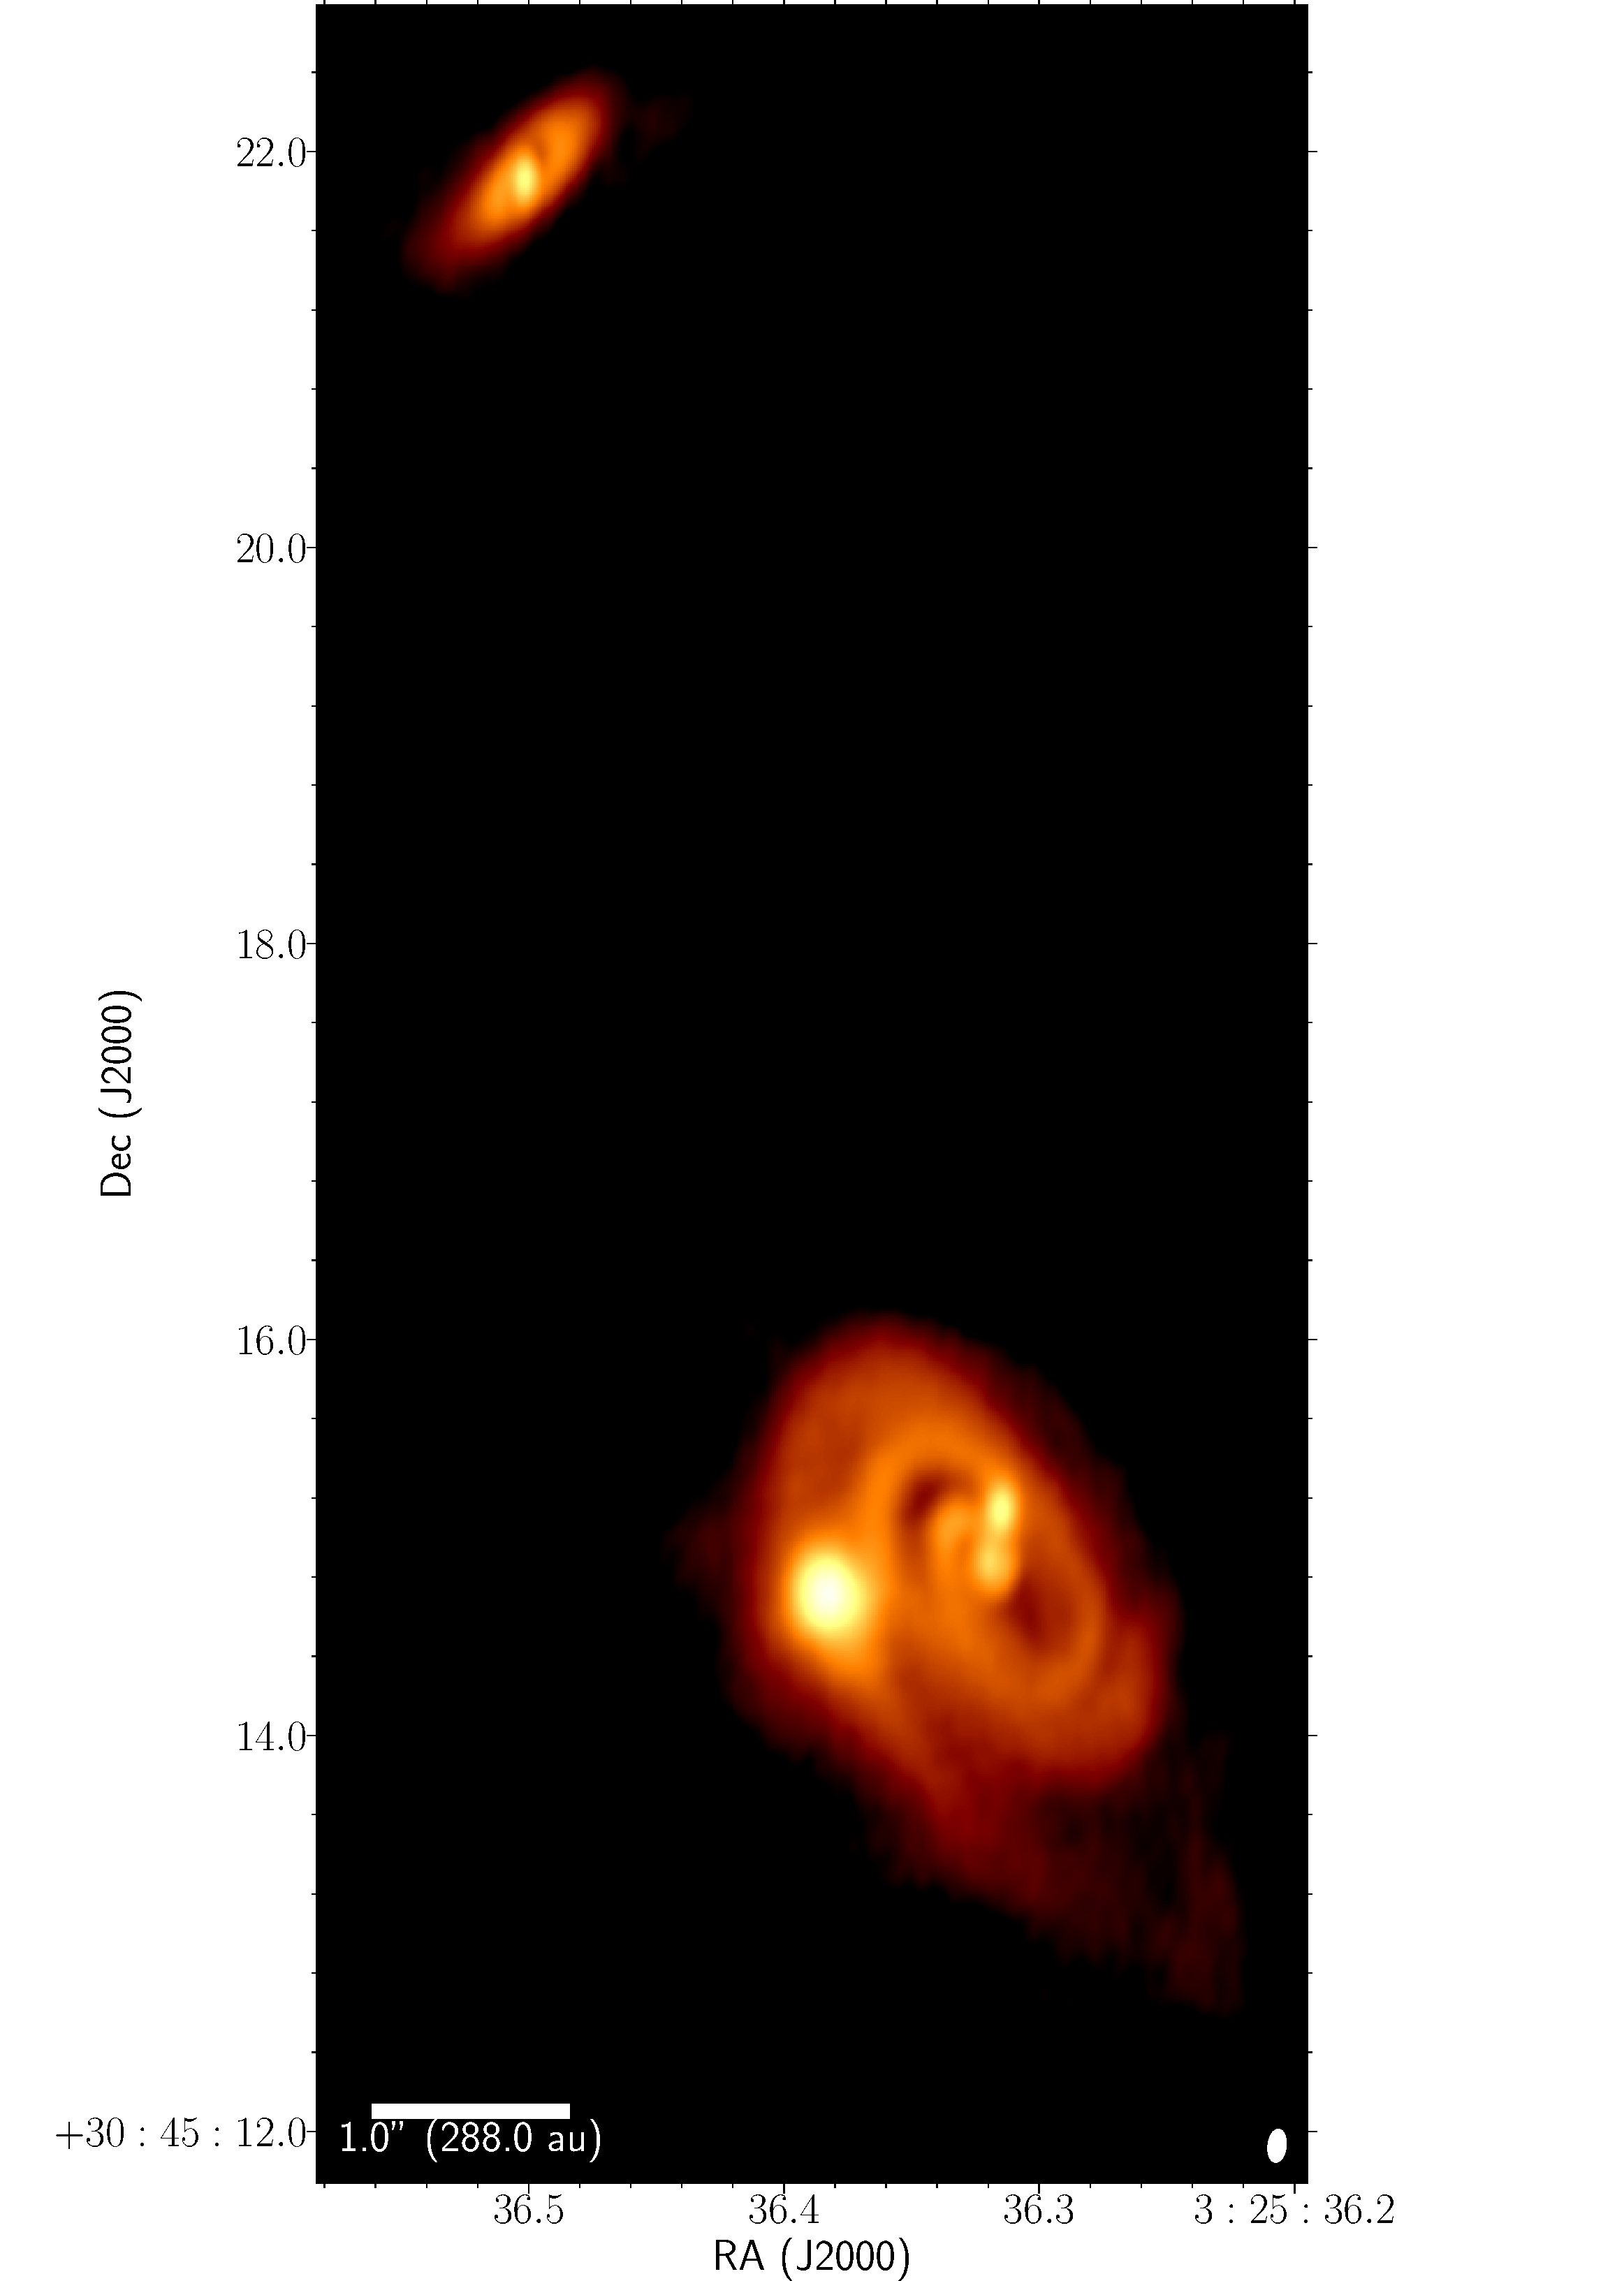
\includegraphics[width=\textwidth]{img/L1448IRS3B_cont_robust05all.pdf}
 \end{minipage}
 \begin{minipage}{0.49\textwidth}
  \vfill
  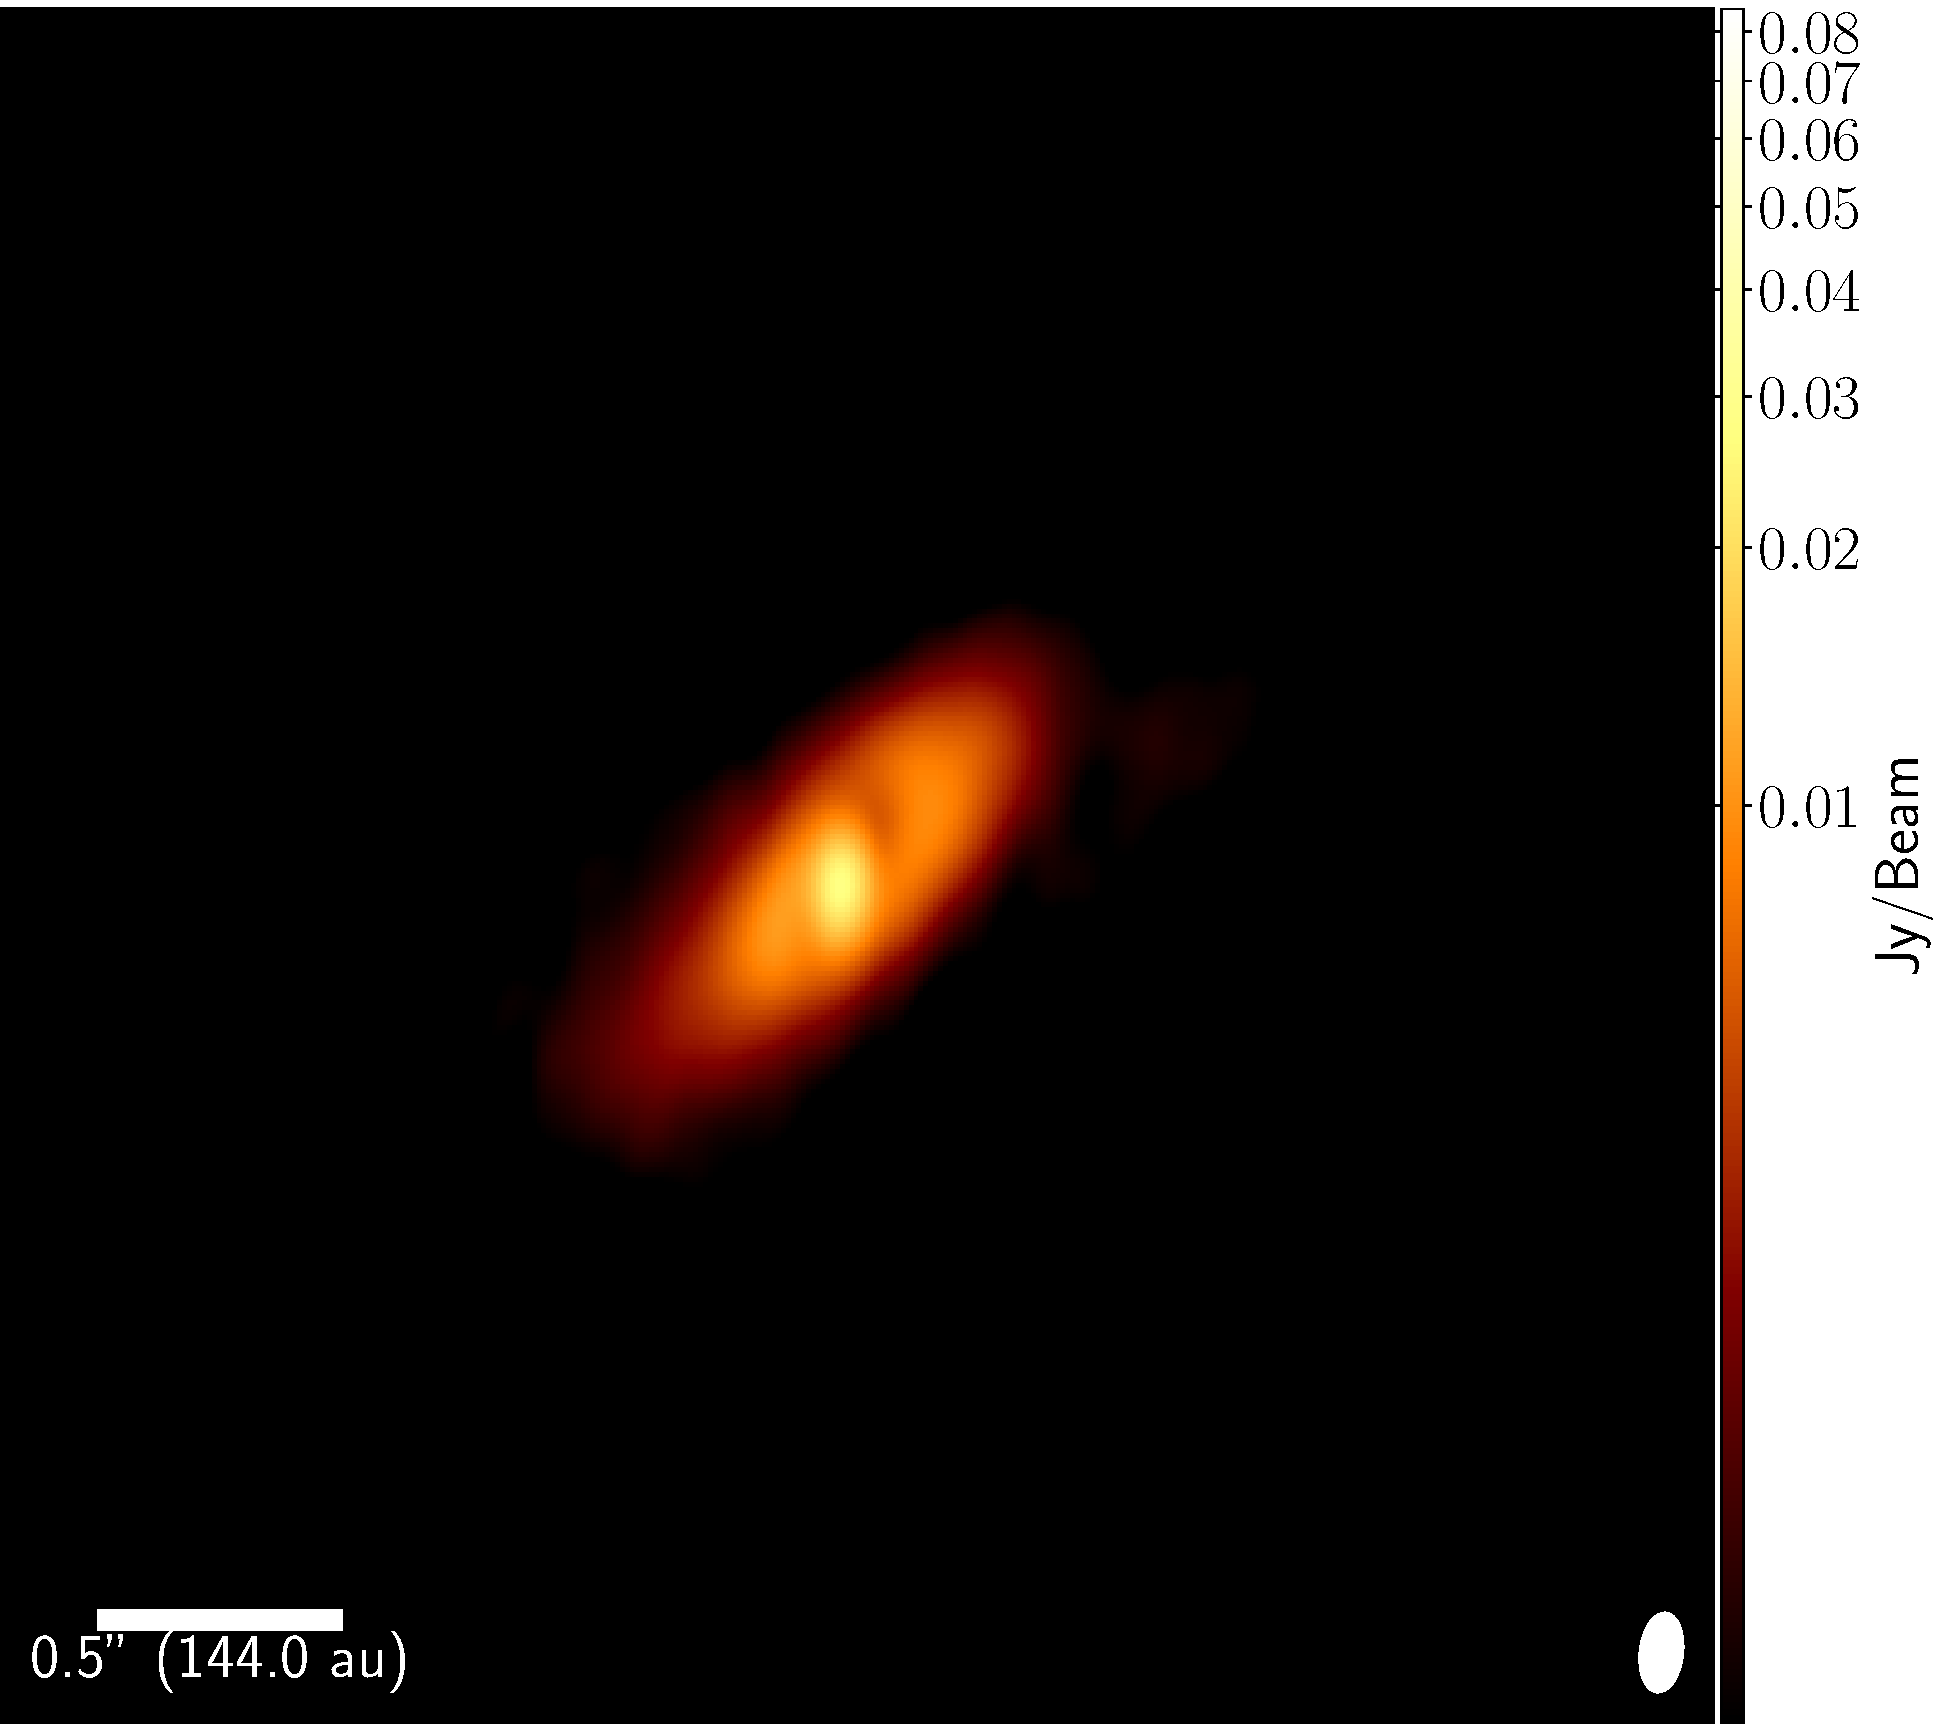
\includegraphics[width=\textwidth]{img/L1448IRS3B_cont_robust05single_uc.pdf}
  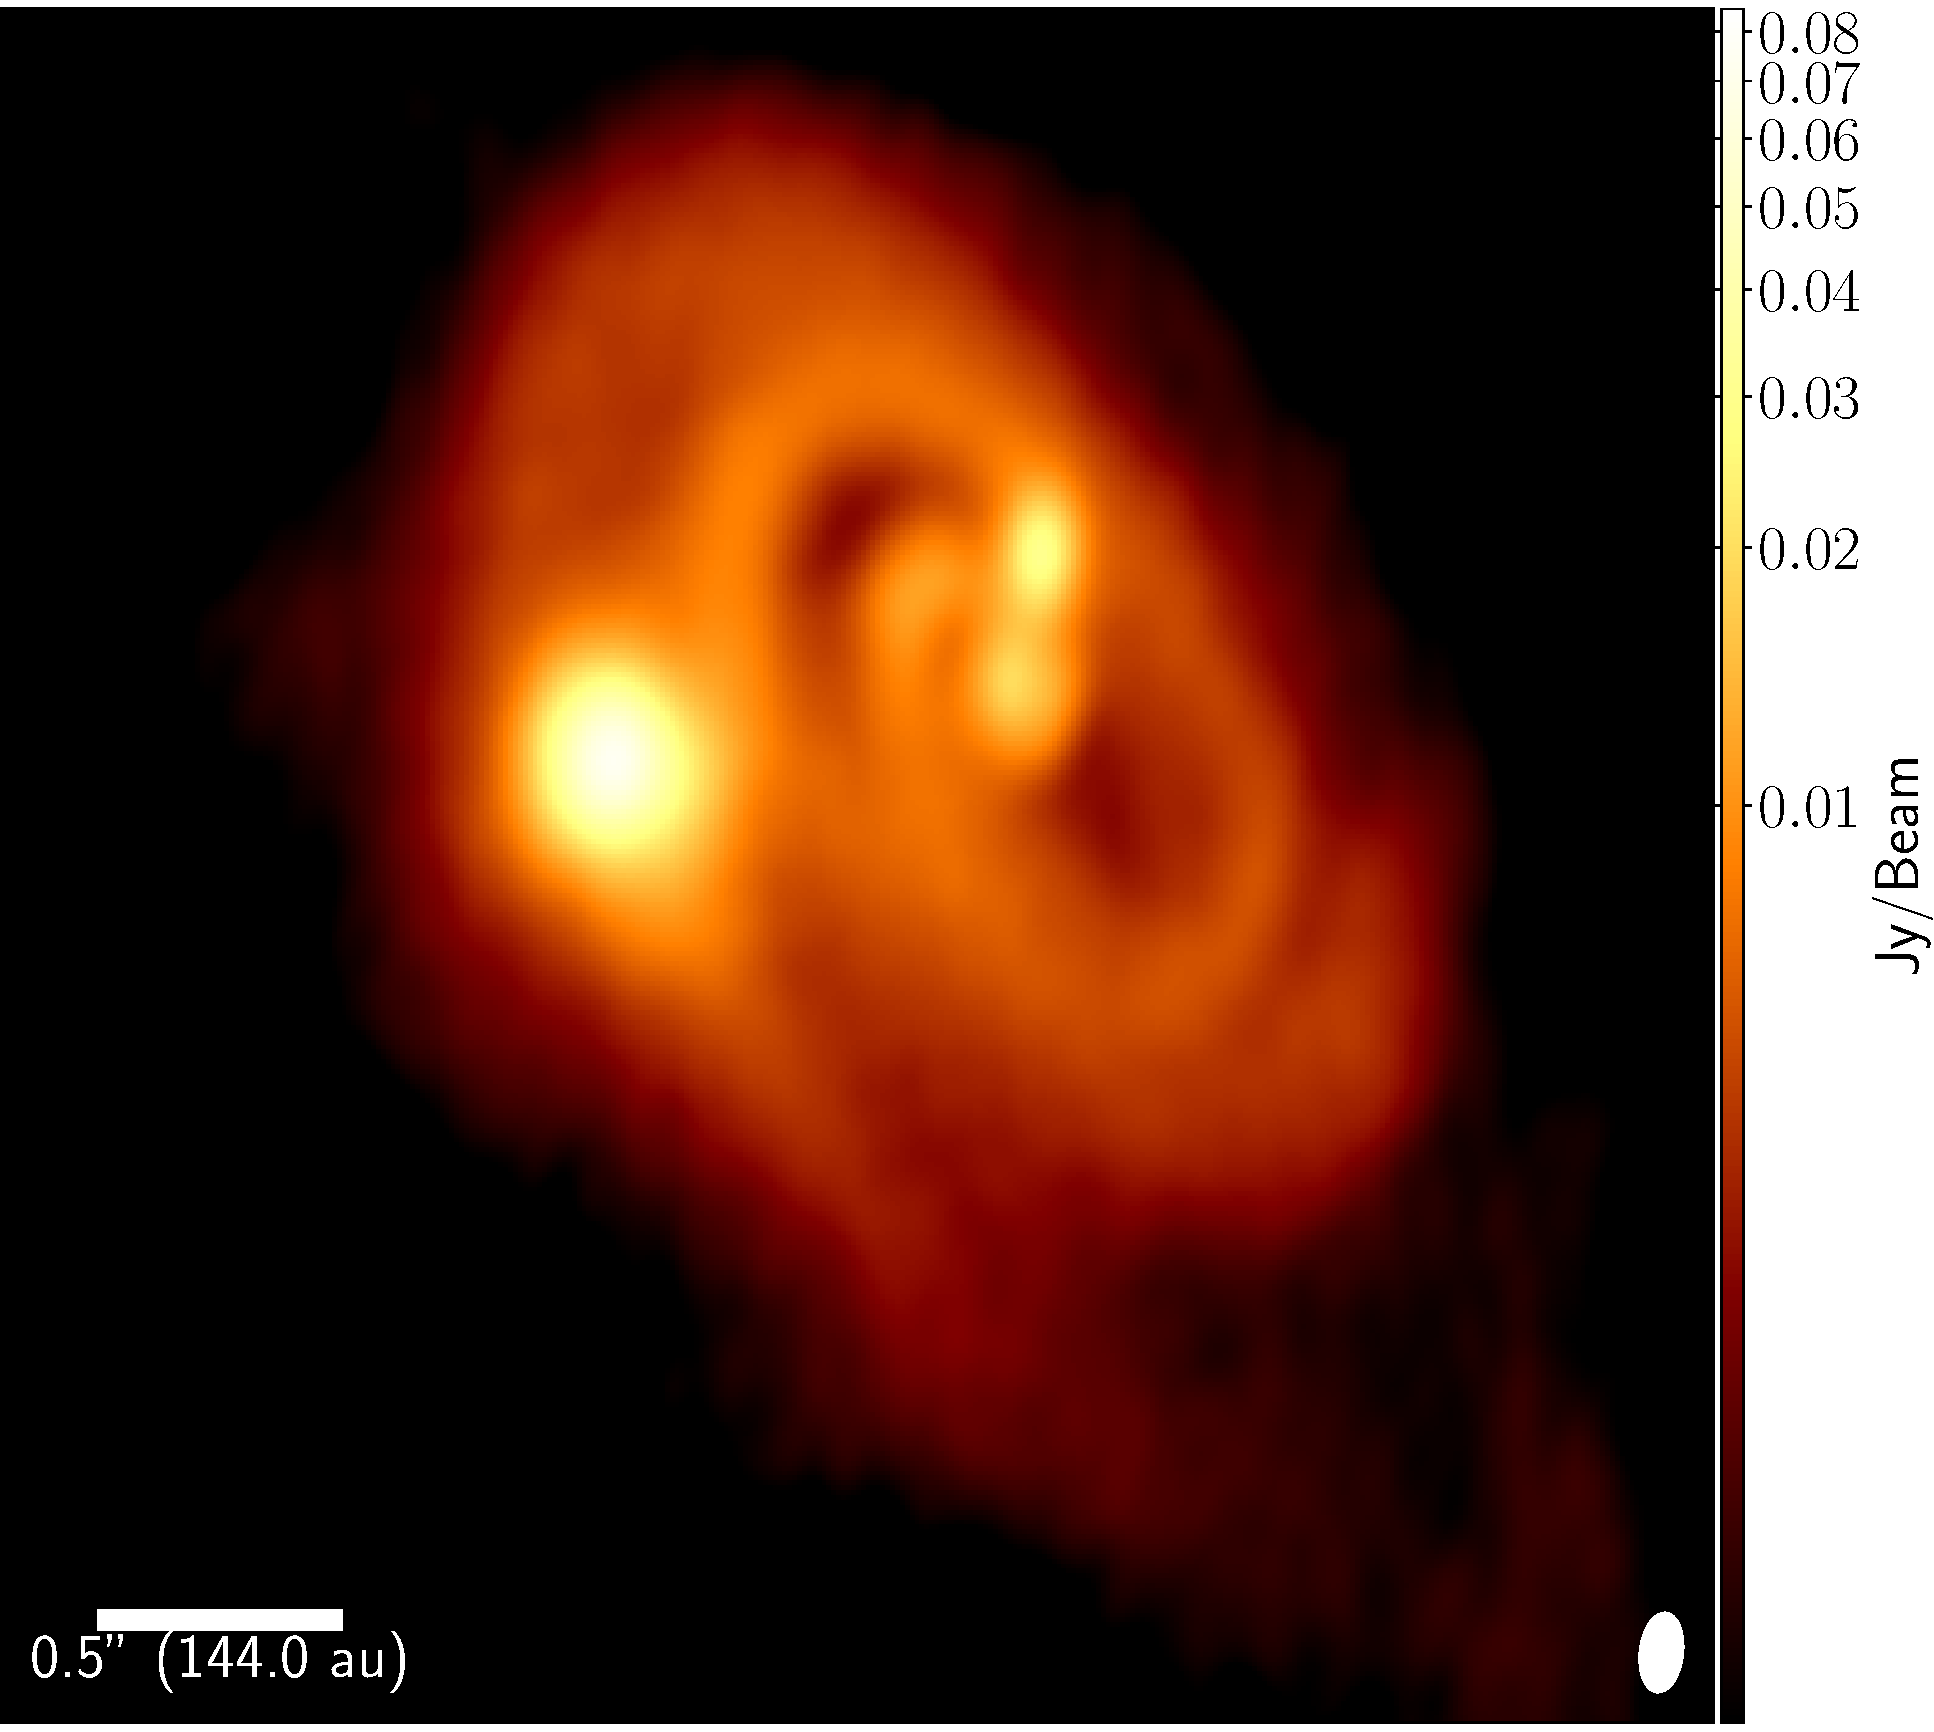
\includegraphics[width=\textwidth]{img/L1448IRS3B_cont_robust05triplet_uc.pdf}
  \vfill
 \end{minipage}
\end{center}
\caption{ALMA 879~\micron\space continuum observations of the triple protostellar system L1448 IRS3B and its wide companion IRS3A (\textbf{left}). The right panels are \ab2$\times$\space zoom-ins on IRS3B~and~IRS3A. The top right image shows the wide companion, IRS3A, (d\ab7\farcs9$\approx$2300~au), featuring possible spiral structure. The bottom right image zooms in on the proto-multiple system, IRS3B. The inner binary is separated by 0\farcs25 (75~au) and has a spiral circum-binary disk with the embedded source \ab0\farcs8 (230~au) away from the binary within one of the arms. The beam size of each panel is shown in lower right (\contbeam).}\label{fig:contimage}
\end{figure}







\begin{figure}[H]
  \begin{center}
   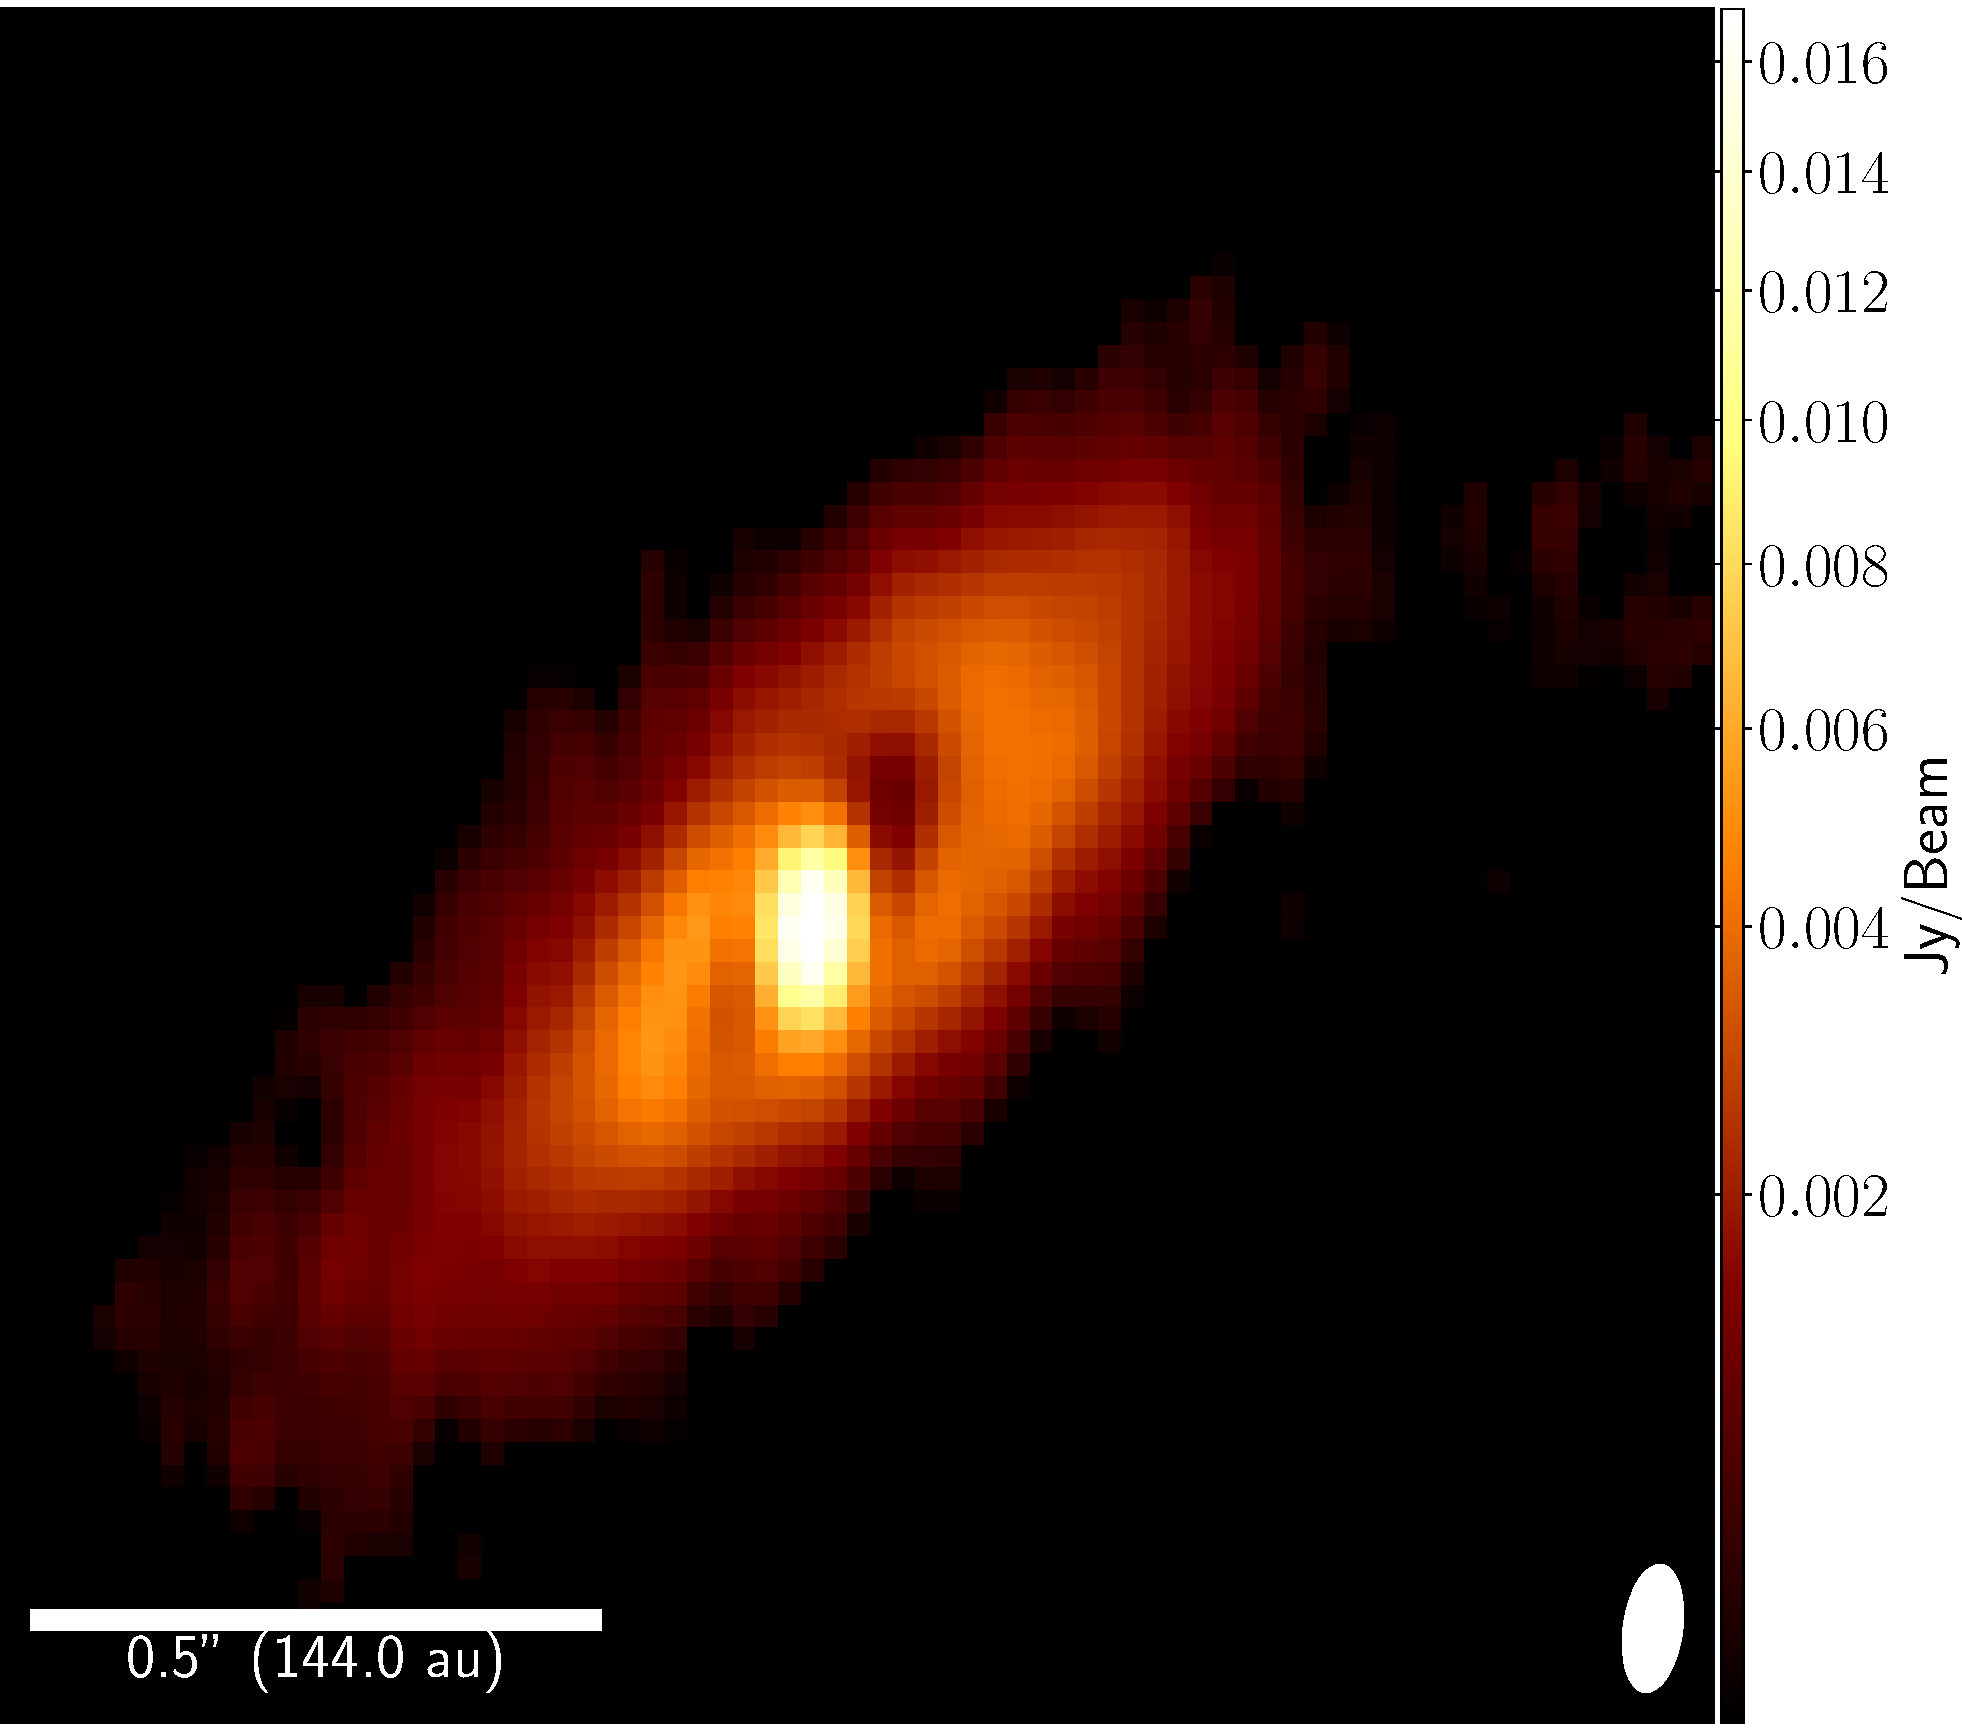
\includegraphics[width=0.48\textwidth]{img/L1448IRS3B_useforsub_widecenter_ms_superuniform_imagesingle_uc-superuniform.pdf} % co
   \end{center}
   \caption{Continuum (879~\micron) image of IRS3A, reconstructed with the \textit{superuniform} weighing scheme and zoomed 2x from the images in Figure~\ref{fig:contimage}\space to highlight the possible spiral substructure.} \label{fig:widesuperuniform}
\end{figure}

% Figure 3
\begin{figure}[H]
\begin{center}
   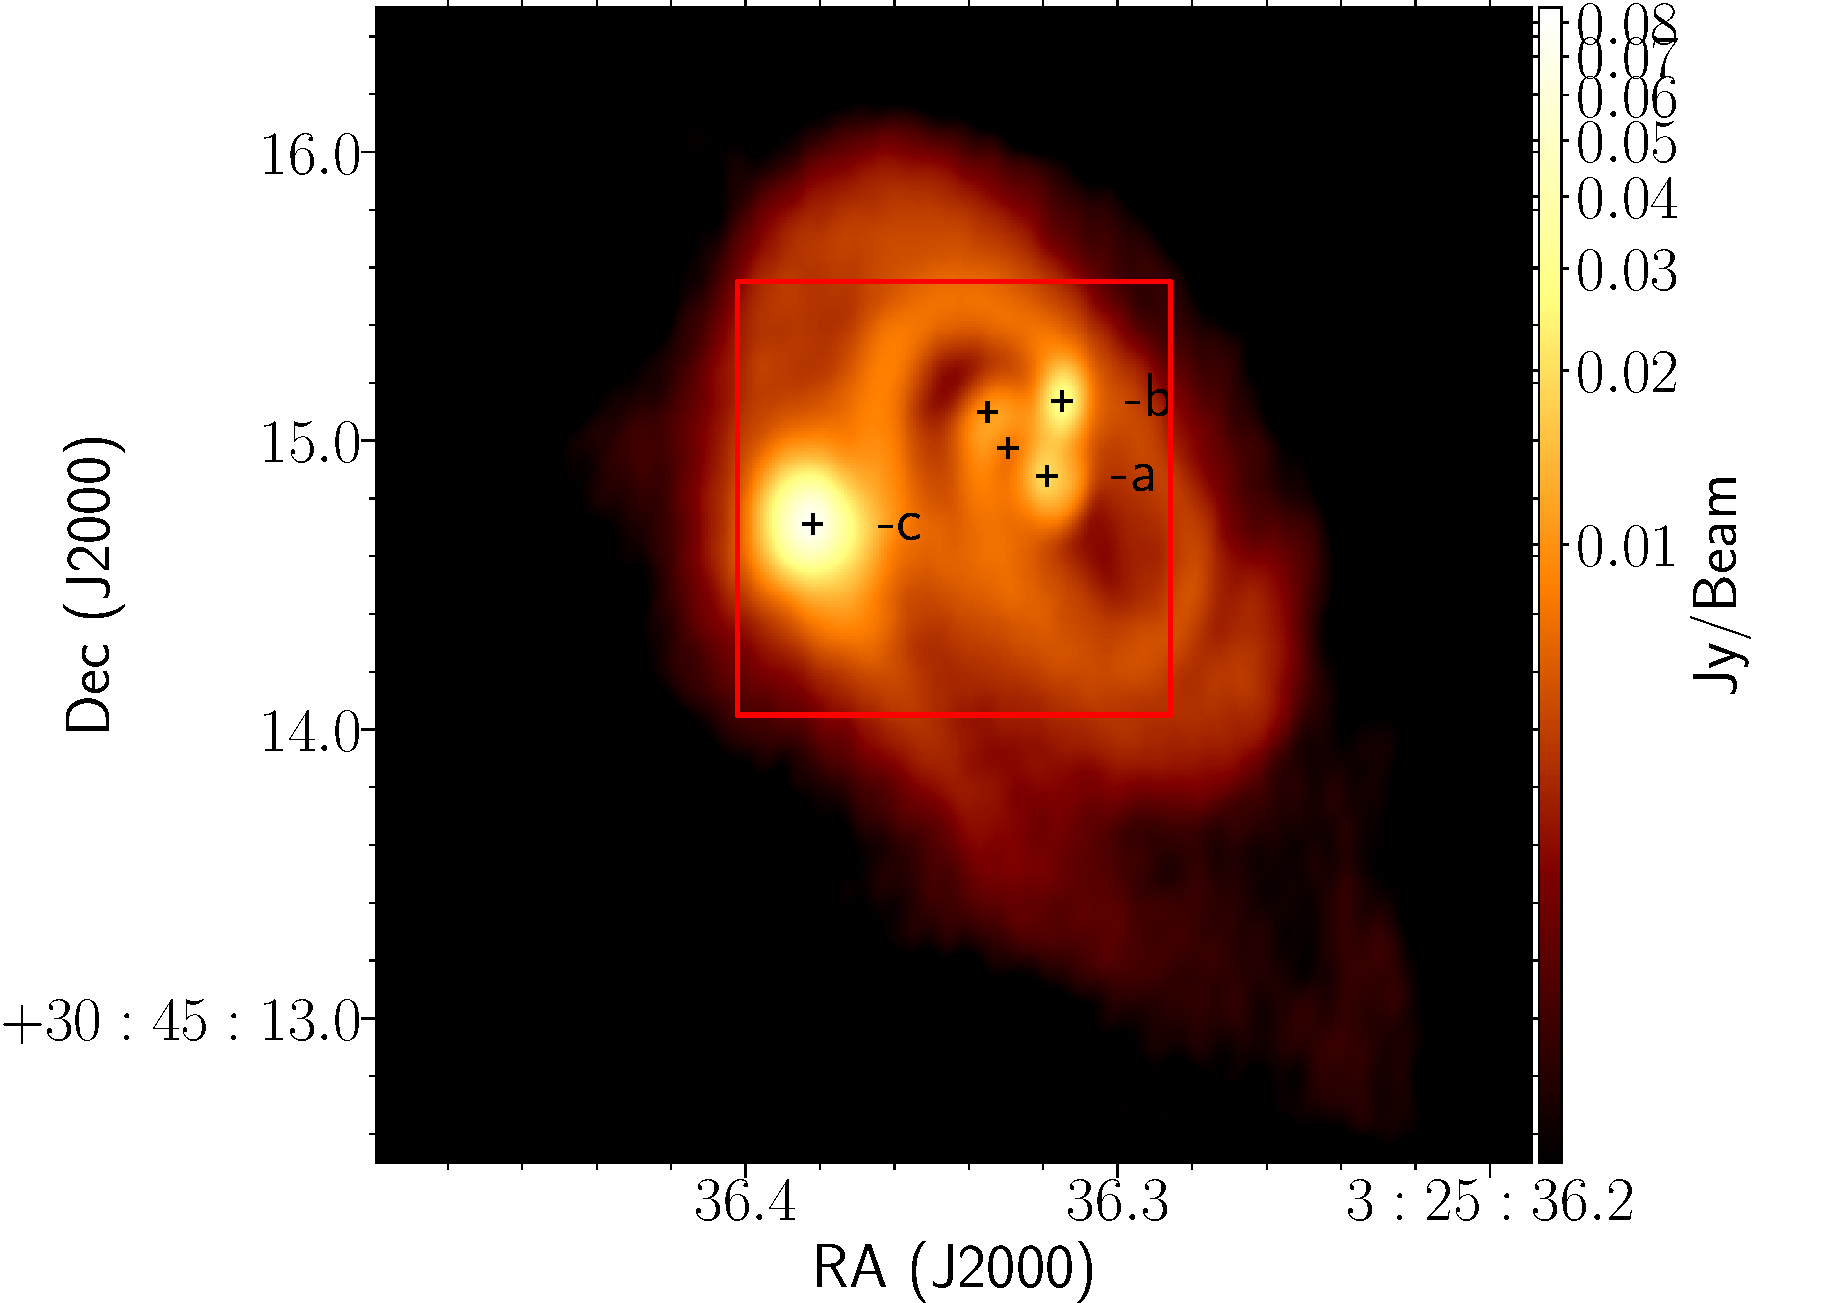
\includegraphics[width=0.48\textwidth]{img/L1448IRS3B_cont_robust05triplet_uc_forpos.pdf} % cont
   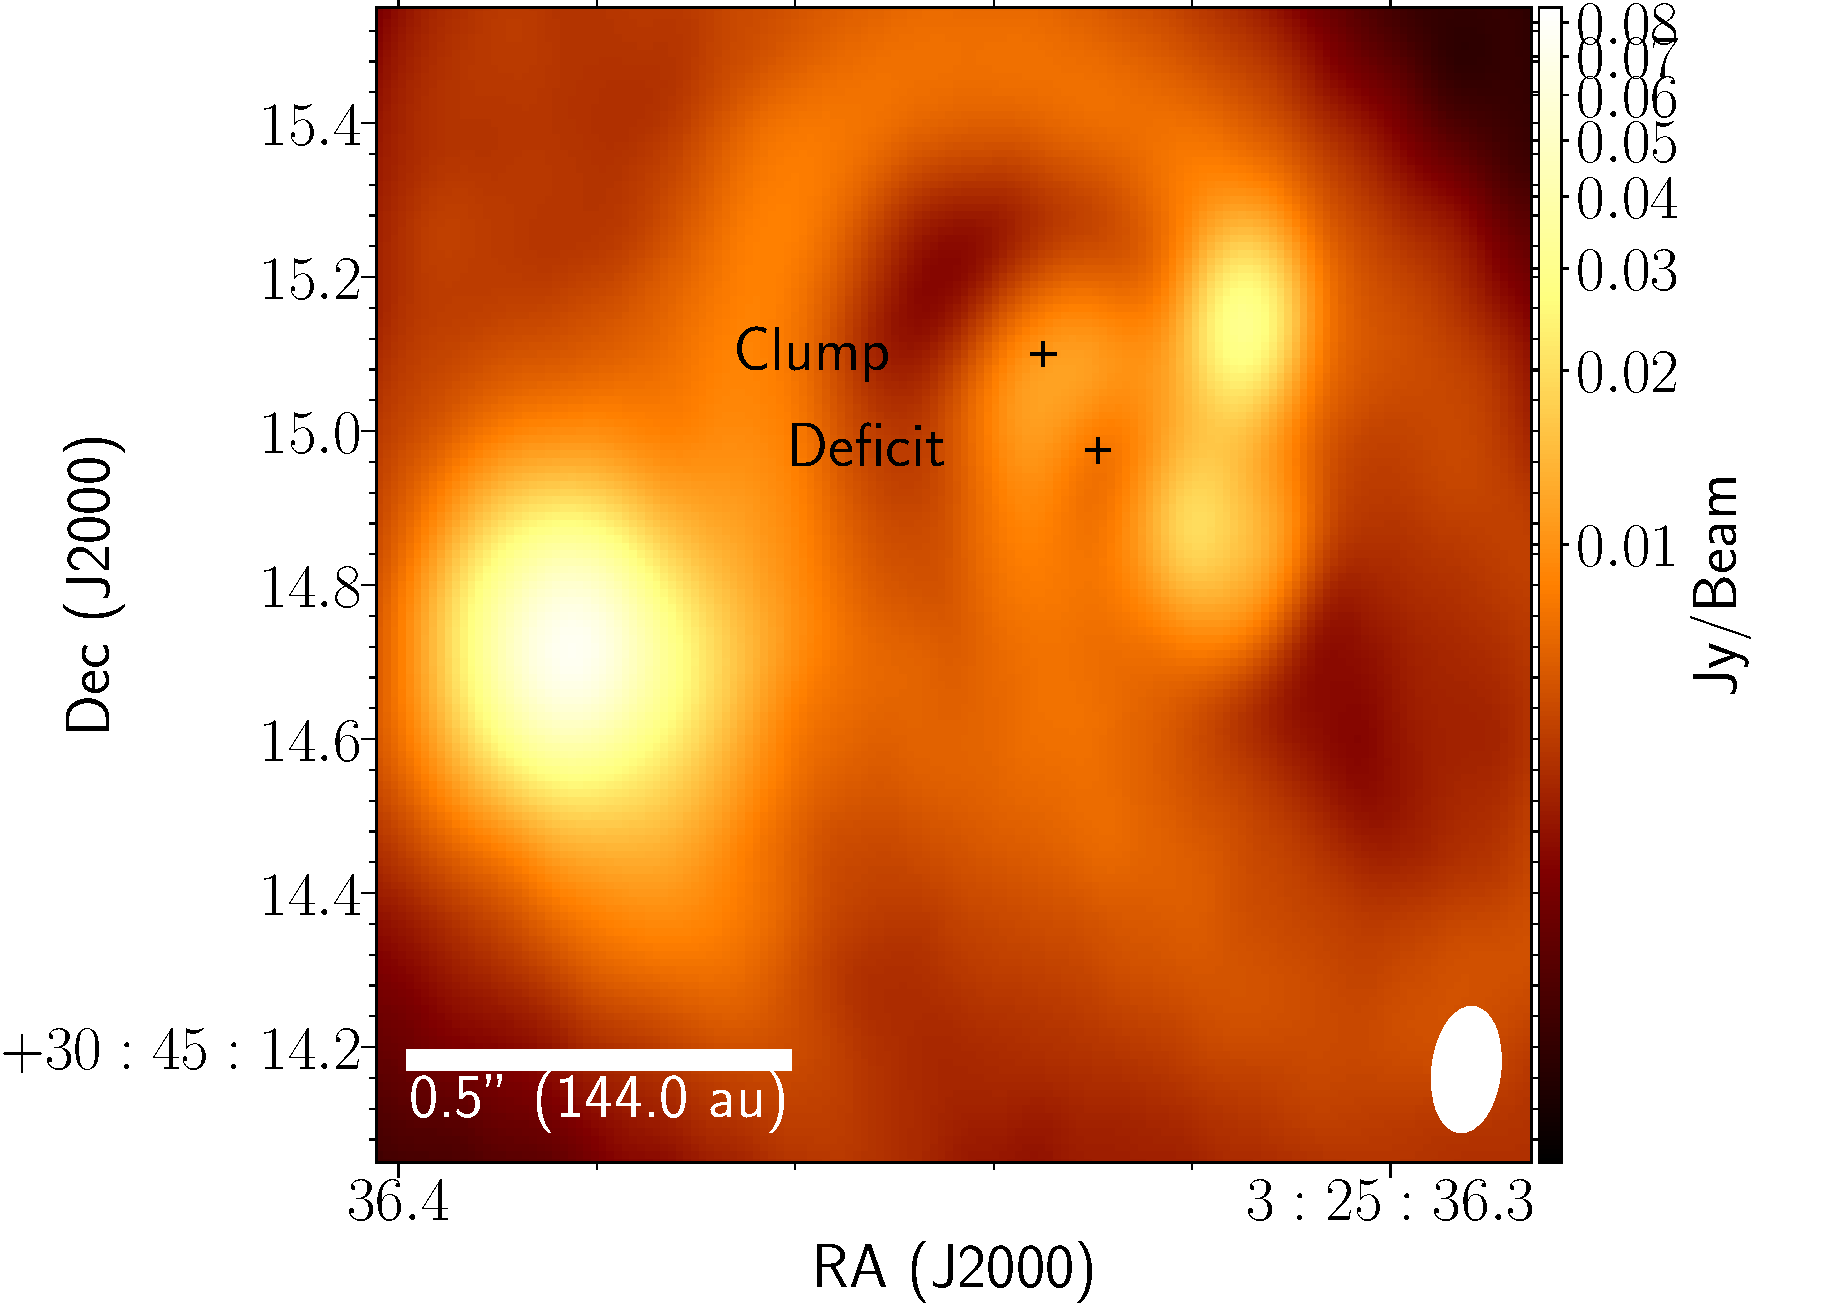
\includegraphics[width=0.48\textwidth]{img/L1448IRS3B_cont_robust05triplet_uc_positions.pdf} % cont
\end{center}
   \caption{ALMA 879~\micron\space continuum observations of the triple protostellar system L1448 IRS3B\added{ with the difference continuum sources marked}. The left colored image is zoomed in on IRS3B and is plotting with a log color stretch. The inner binary is separated by 0\farcs25 (75~AU) and has a circum-binary disk with spiral structure and the tertiary is separated from the binary by \ab0\farcs8 (230~AU) within one of the arms. The ``protostars'' are the continuum positions previously discovered in \citet{2016Natur.538..483T}, while the ``clump'' is a new feature, resolved in these observations. The ``deficit'' indicates the location of depression of flux between IRS3B-a and the ``clump''. This is discussed in Sections~\ref{sec:dcont}~and~\ref{sec:discussion}. The beam size of each panel is shown in lower right (\contbeam\space using Briggs Robust parameter of 0.5).}\label{fig:zoomincont}
\end{figure}







% Figure 2
\begin{figure}[H]
\begin{center}
   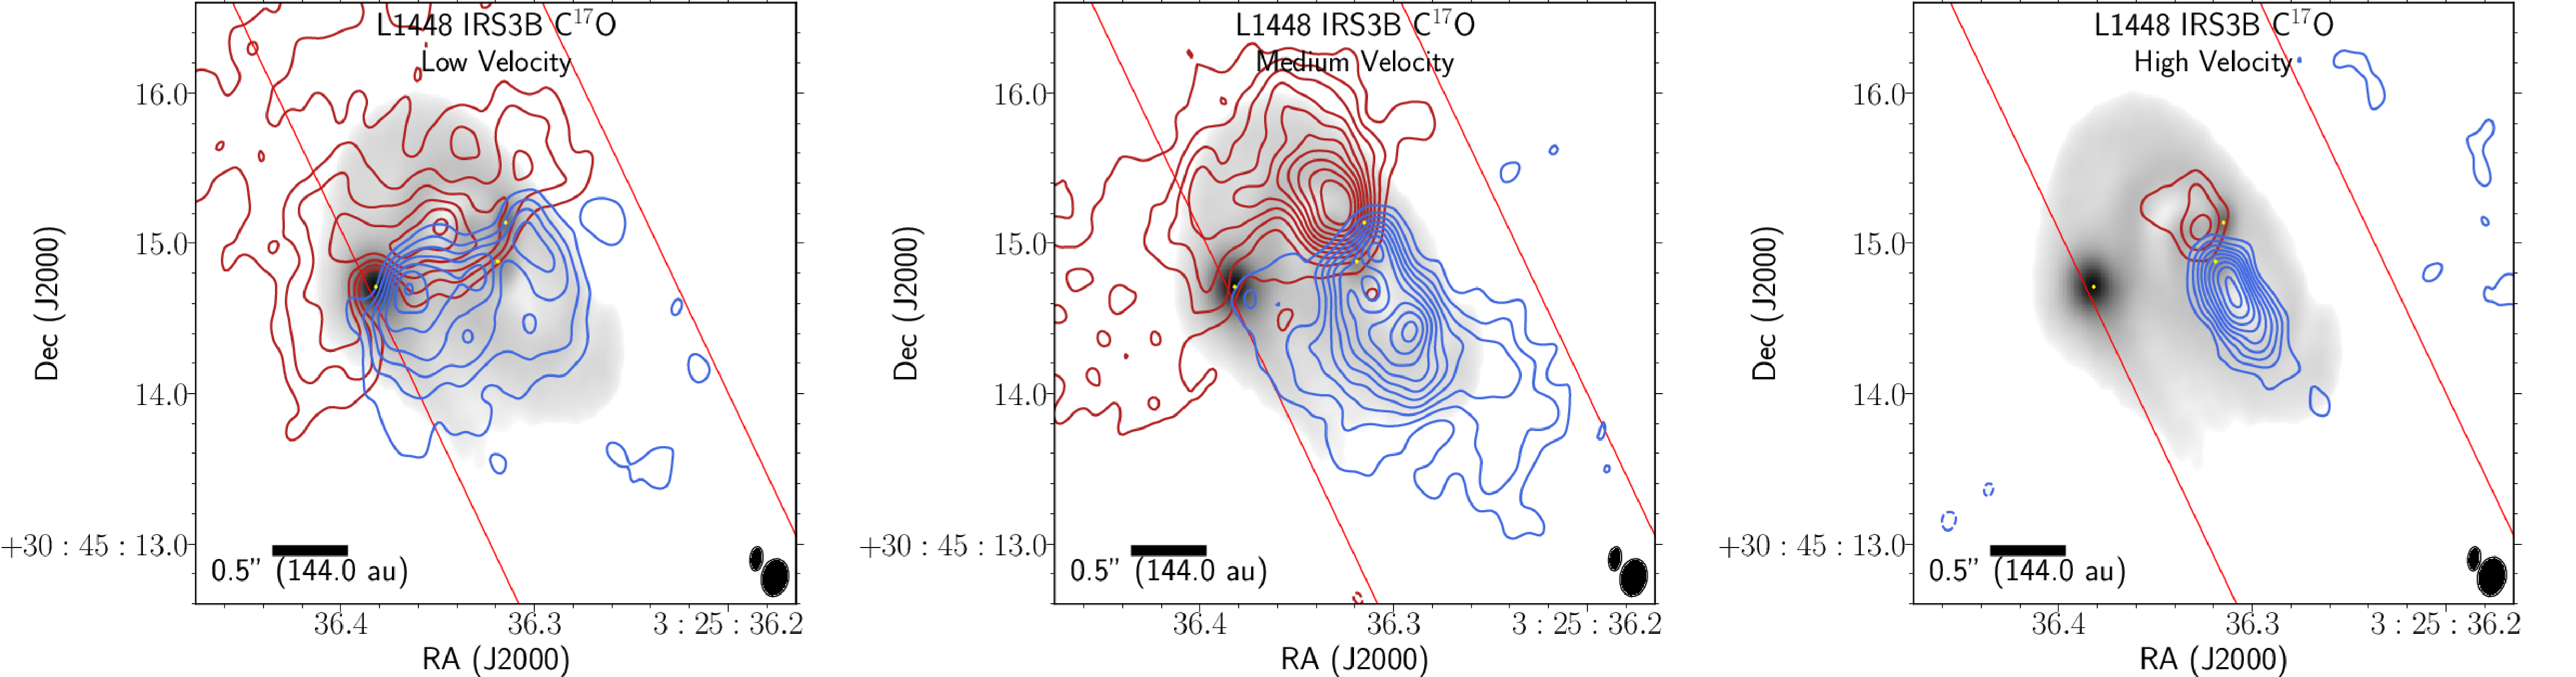
\includegraphics[width=1\textwidth]{img/L1448IRS3B_C17O_image_taper1500k__splitMoments_panel.pdf}  % c17o
\end{center}
   \caption{\cso\space integrated intensity maps towards IRS3B over a selected range of velocities overlayed on continuum (grayscale). The \cso\space emission traces the rotating gas within the disk via Doppler-shifted emission. The panels correspond to low, medium, and high velocity ranges which are delineated as red(blue), respectively. Negative contours are not present in these integrated intensity maps; however, at the location of IRS3B-c, there is strong absorption that is evident in the high spectral resolution data cube, but is not represented here. The red lines indicate the region extracted for PV diagram construction, along the position angle of the major axis. \textbf{Low Velocity:} Velocity range starts at 4.68$\rightarrow$5.67~\kms (3.58$\rightarrow$4.68~\kms) and contours start at 8(8)$\sigma$ and iterate by 3(3)$\sigma$ with the 1$\sigma$~level starting at 0.0023(0.0025)~Jy~beam$^{-1}$ for the red(blue) channels respectively. \textbf{Medium Velocity:} Velocity range starts at 5.67$\rightarrow$6.66~\kms (2.48$\rightarrow$3.58~\kms) and contours start at 3(5)$\sigma$ and iterate by 3(3)$\sigma$ with the 1$\sigma$~level starting at 0.002(0.0016)~Jy~beam$^{-1}$ for the red(blue) channels respectively. \textbf{High Velocity:} Velocity range starts at 6.66$\rightarrow$7.65~\kms (1.27$\rightarrow$2.48~\kms) and contours start at 5(5)$\sigma$ and iterate by 3(3)$\sigma$ with the 1$\sigma$~level starting at 0.0018(0.0012)~Jy~beam$^{-1}$ for the red(blue) channels respectively. The \cso\space synthesized beam (\csobeam) is the bottom-right most ellipse on each of the panels and the continuum synthesized beam (\contbeam) is offset diagonally.}\label{fig:irs3bc17omoment}
\end{figure}





% Figure 8
% irs3a
\begin{figure}[H]
\begin{center}
   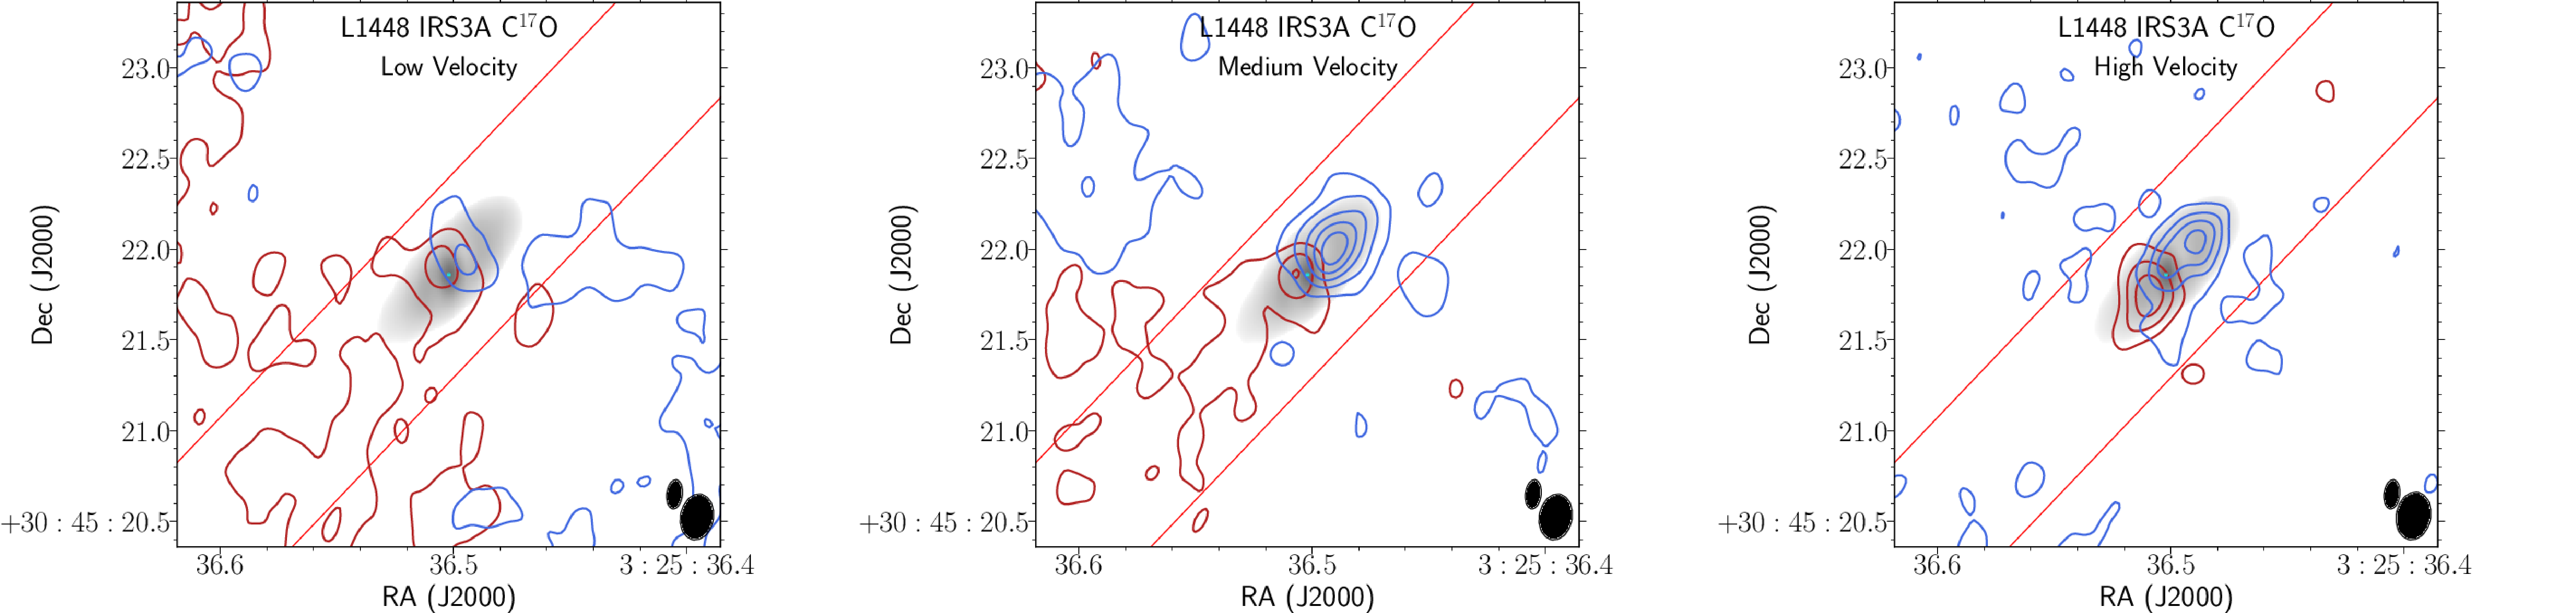
\includegraphics[width=1\textwidth]{img/L1448IRS3B_C17O_image_taper1500k__-irs3asplitMoments_irs3a_panel.pdf}  % c17o
\end{center}
   \caption{\cso\space integrated intensity maps toward IRS3A over a selected range of velocities overlayed on continuum (grayscale). The \cso\space emission exhibits a velocity gradient across the continuum emission. However, S/N is low in comparison to IRS3B. The panels correspond to low, medium, and high velocity ranges which are delineated as red(blue), respectively. The red lines indicate the region extracted for PV diagram construction, along the position angle of the major axis. \textbf{Low Velocity:} velocity ranges 5.2$\rightarrow$6.5~\kms (4.1$\rightarrow$5.2~\kms), contours start at 3(3)$\sigma$ and iterate by 3(3)$\sigma$ with the 1$\sigma$~level starting at 0.0023(0.0025)~Jy~beam$^{-1}$ for the red(blue) channels respectively. \textbf{Medium Velocity:}  velocity ranges 6.5$\rightarrow$7.4~\kms (3.0$\rightarrow$4.1~\kms), contours start at 3(3)$\sigma$ and iterate by 3(3)$\sigma$ with the 1$\sigma$~level starting at 0.002(0.0016)~Jy~beam$^{-1}$ for the red (blue) channels respectively. \textbf{High Velocity:} velocity ranges 7.4$\rightarrow$8.6~\kms (1.8$\rightarrow$3.0~\kms), contours start at 3(3)$\sigma$ and iterate by 3(3)$\sigma$ with the 1$\sigma$~level starting at 0.0018(0.0012)~Jy~beam$^{-1}$ for the red(blue) channels respectively. The \cso\space synthesized beam (\csobeam) is the bottom-right most ellipse on each of the panels and the continuum synthesized beam (\contbeam) is offset diagonally.}\label{fig:irs3ac17omoment}
\end{figure}

% Figure 8
% irs3a
\begin{figure}[H]
\begin{center}
   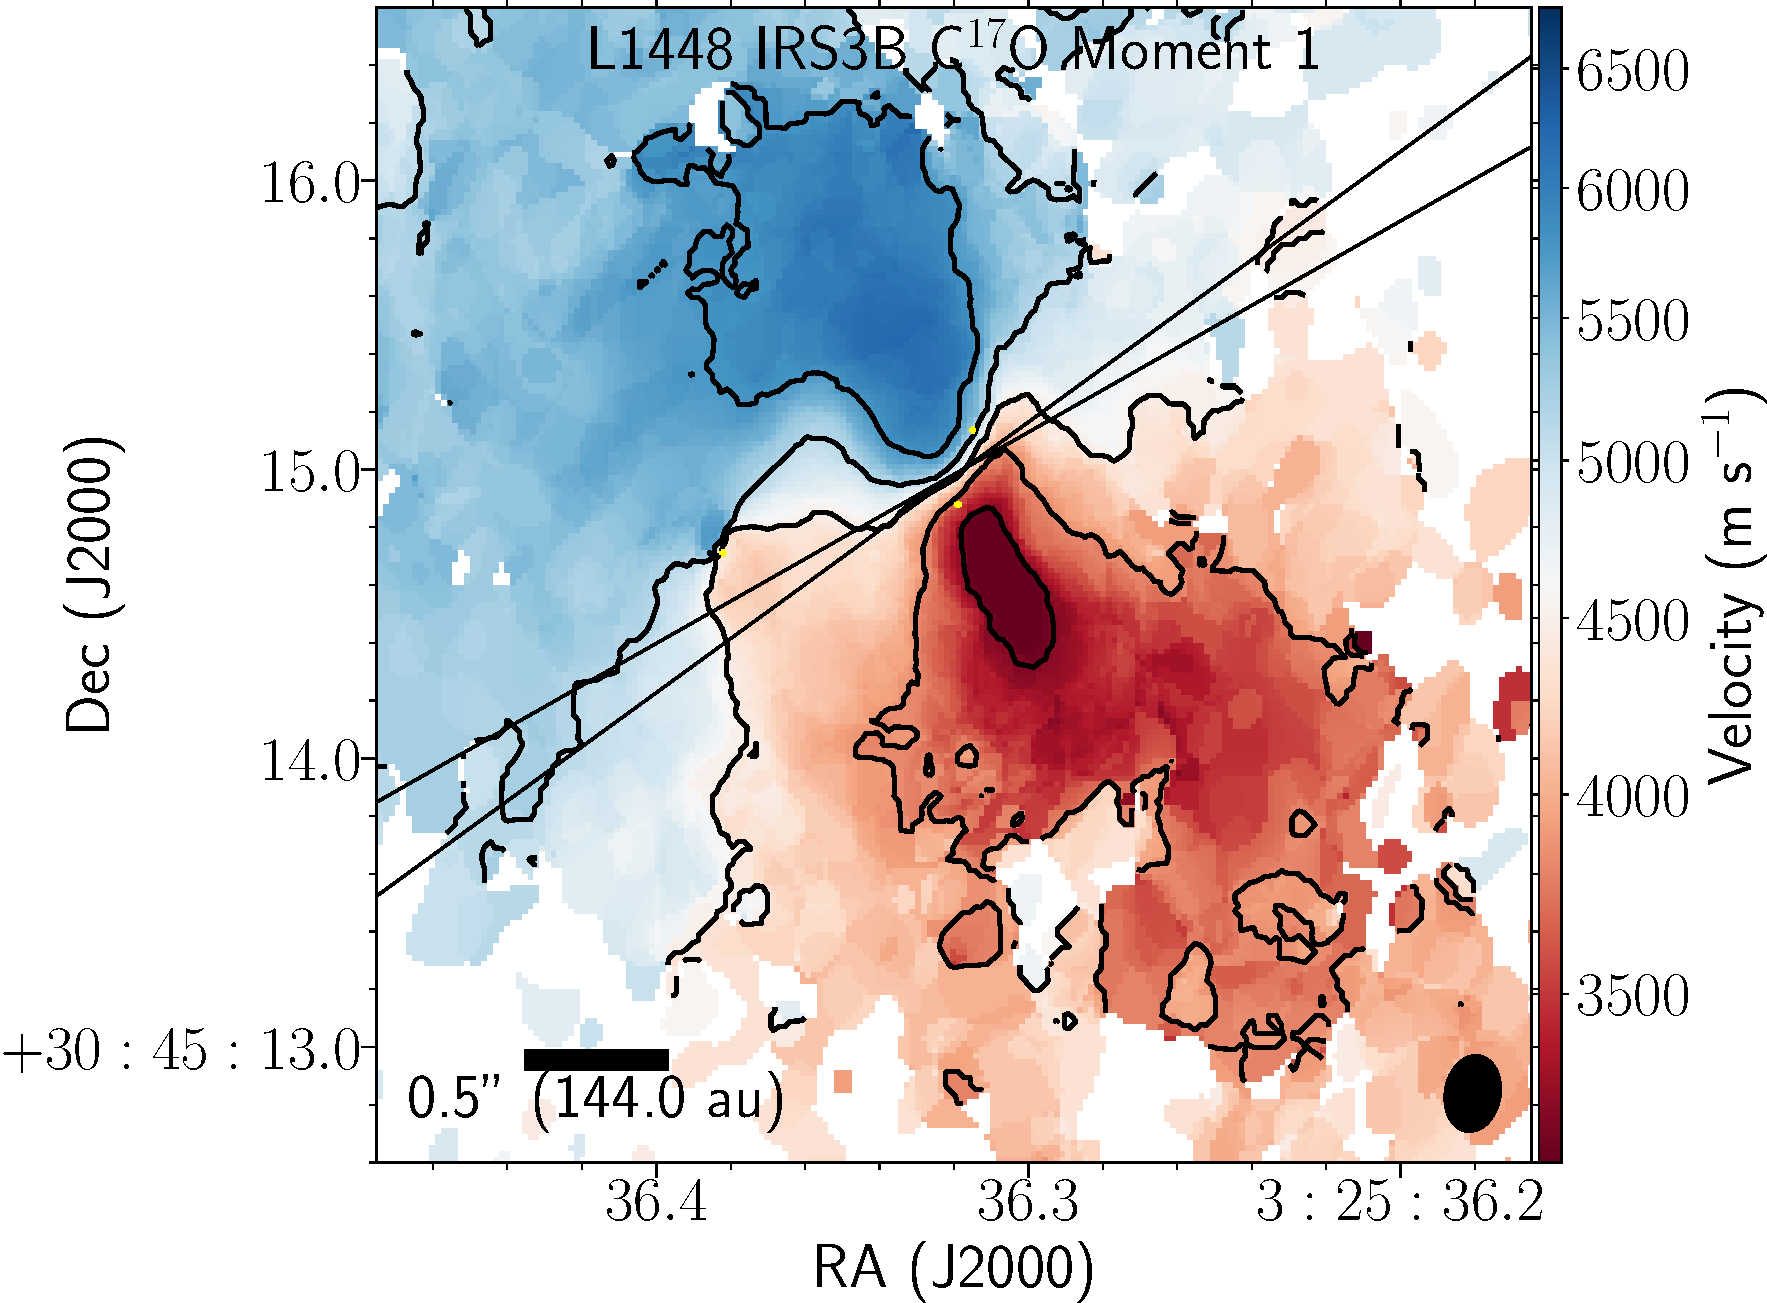
\includegraphics[width=1\textwidth]{img/L1448IRS3B_C17O_image_taper1500k_image_M1_fits.pdf}  % c17o
\end{center}
   \caption{\cso\space velocity-weighted integrated intensity maps toward IRS3B and IRS3A over a selected range of velocities (1.27$\rightarrow$7.65~\kms) The \cso\space emission appears well ordered across the semi-major axis. The contours start at 3$\sigma$ and iterate by 1$\sigma$ with the 1$\sigma$~level starting at 0.65~\kms. The yellow markers indicate the three continuum sources. \added{The black lines indicate the position angle estimates as given by the \pdspy\space fitting routine in Table~\ref{table:pvtable}, of $26.7^{+  1.8}_{-  2.9}$\deg.} The \cso\space synthesized beam (\csobeam) is the bottom-right most ellipse.}\label{fig:irs3abc17omoment1}
\end{figure}


% Figure 4
\begin{figure}[H]
\begin{center}
   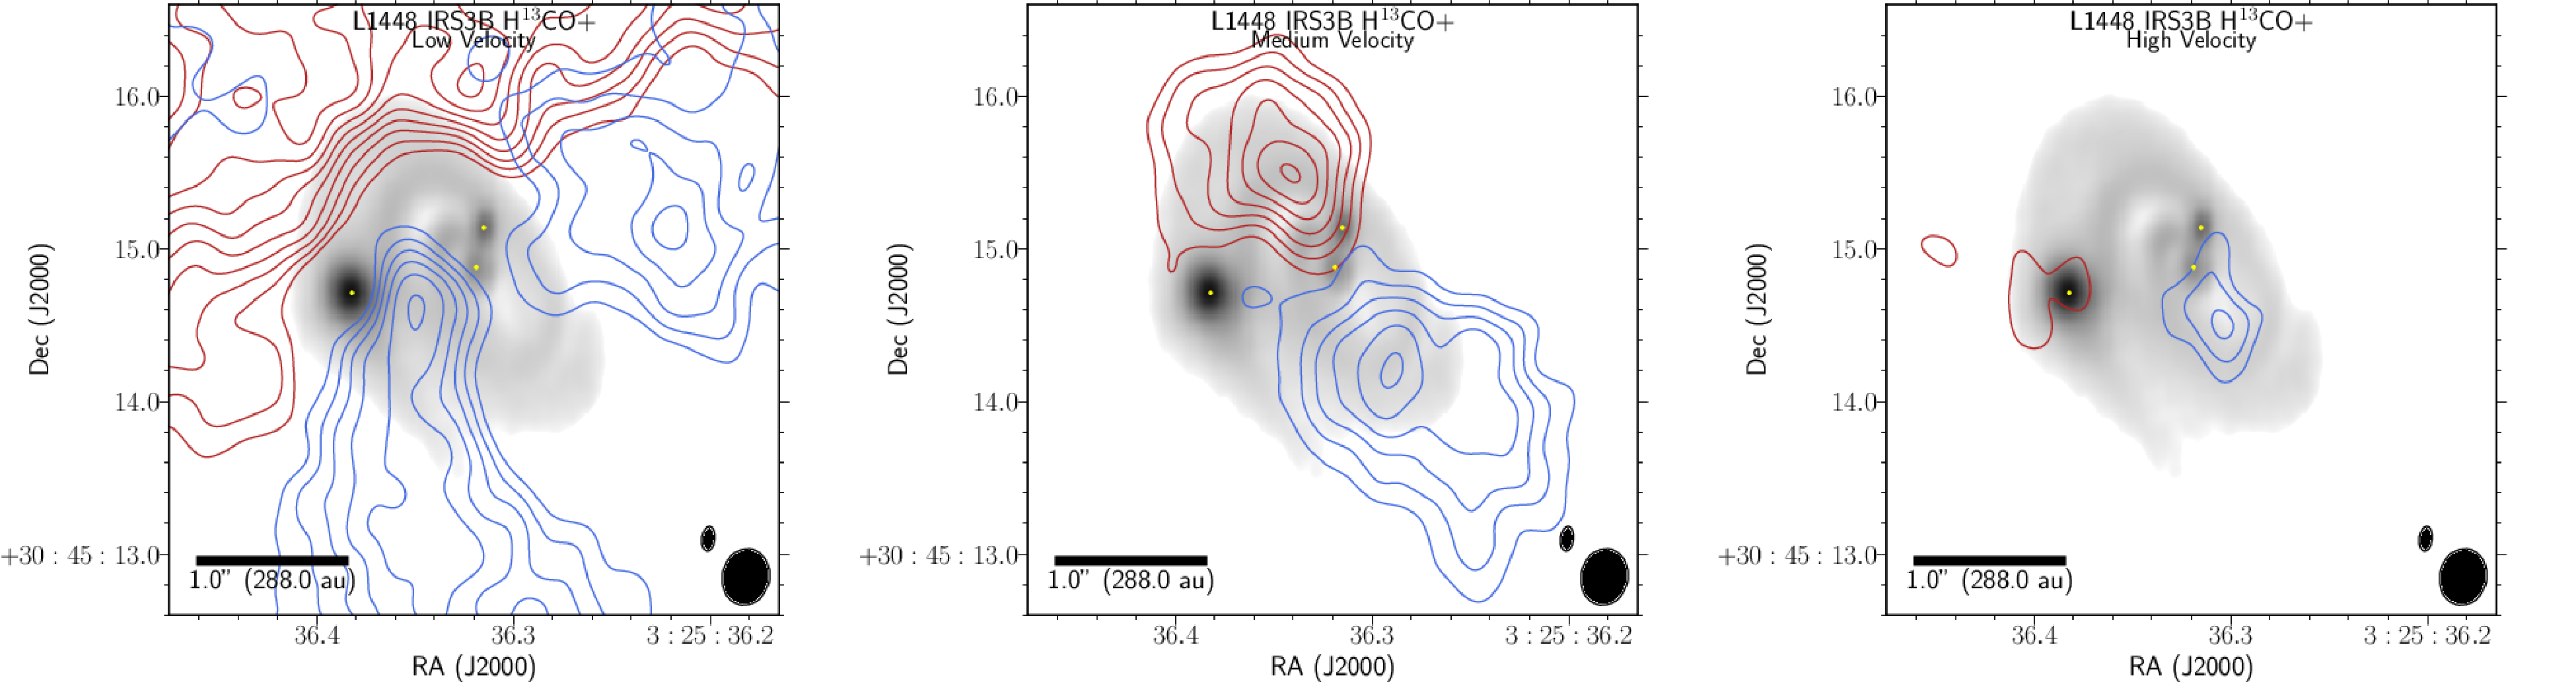
\includegraphics[width=1\textwidth]{img/L1448IRS3B_H13COp_image_taper400k__binned_panel_matchC17O_400.pdf}  % c17o
   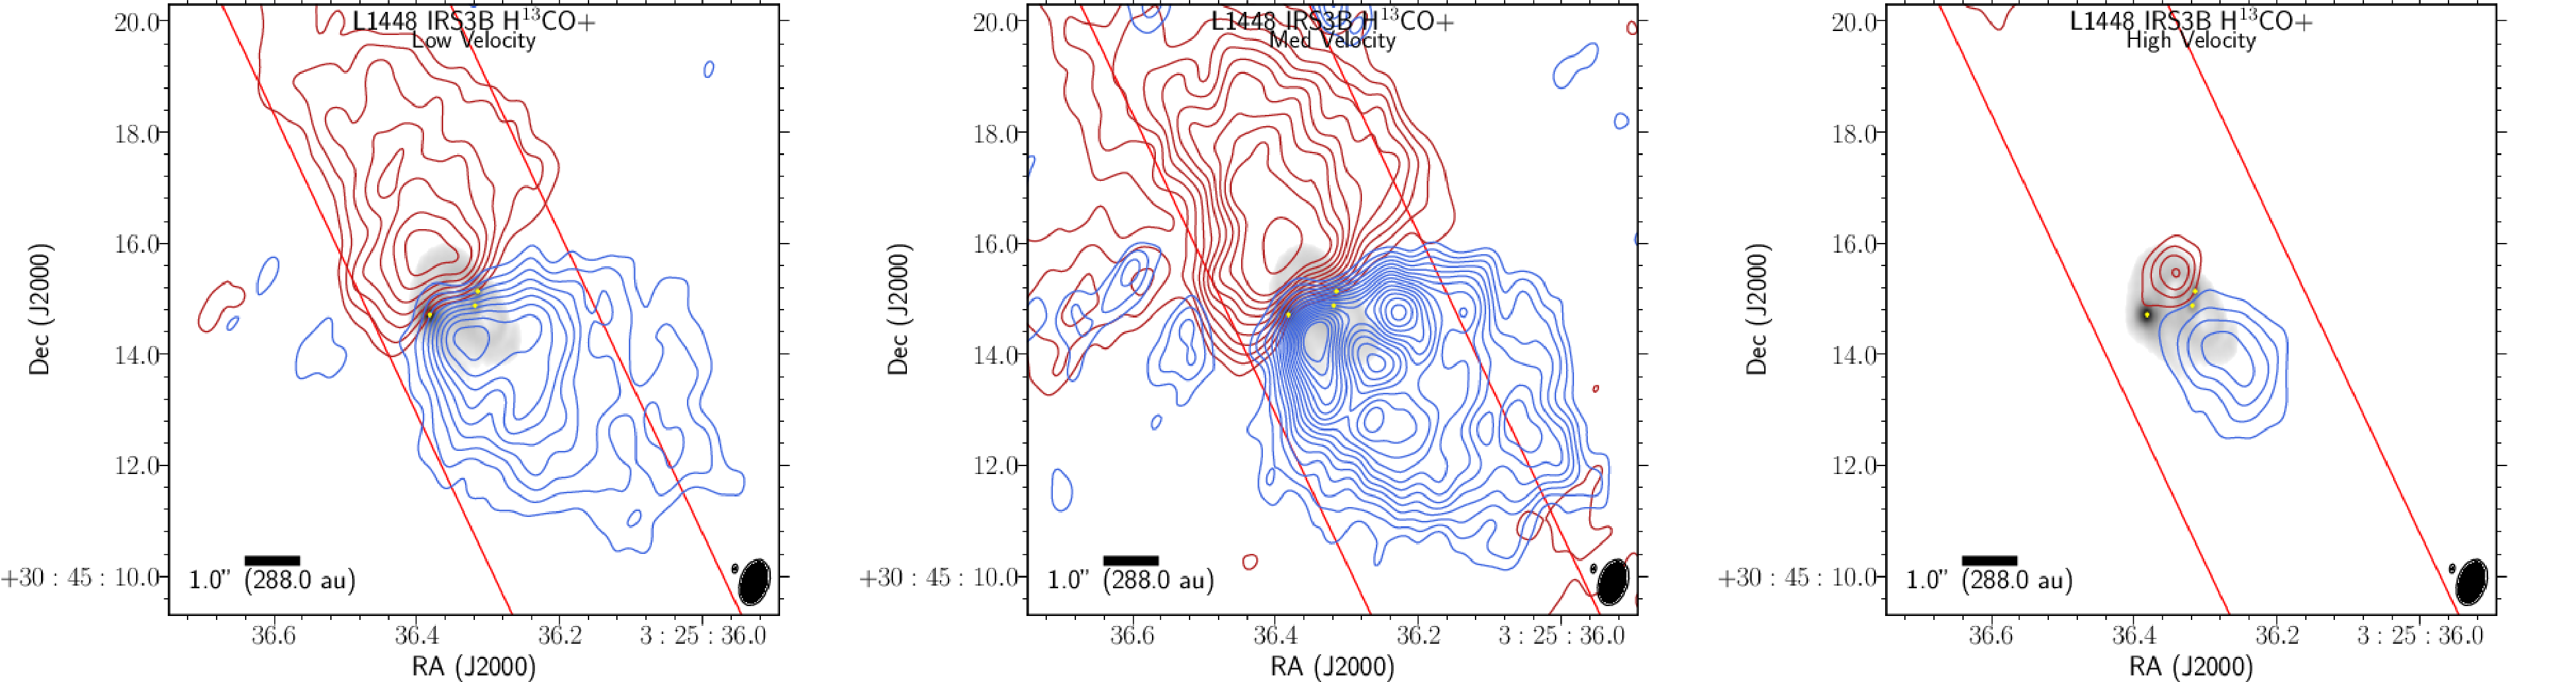
\includegraphics[width=1\textwidth]{img/L1448IRS3B_H13COp_image_taper1000k__binned_panel.pdf}
\end{center}
   \caption{\htcop\space integrated intensity maps towards IRS3B over a selected range of velocities overlayed on continuum (grayscale). The top row spatial scale is set to match those of Figure~\ref{fig:irs3bc17omoment} and the bottom row scale is set to encapsulate the entire IRS3B system, to better demonstrate the spatial scales probed with this molecule. The top row is tapered with a 400~k$\lambda$\space Gaussian to best reduce the amount of noise and show the proper resolution to the spatial scales shown. The \htcop\space emission is primarily tracing the intermediate dense, gaseous material within the inner envelope, but the higher-velocity emission does originate near the protostars. The columns correspond to similar velocity ranges of \cso\space emission as shown in the previous figure, with low, medium, and high Doppler-shifted velocity ranges delineated as red(blue), respectively. Negative contours do not show additional structure and are suppressed for visual aid. The red lines indicate the region extracted for PV diagram construction, along the position angle of the major axis in a region much larger than the \cso\space PV diagram extraction to fully capture the emission. \textbf{Low Velocity:} velocity ranges 4.7$\rightarrow$5.7~\kms (3.6$\rightarrow$4.7~\kms)), contours start at 10(10)$\sigma$ and iterate by 2(2)$\sigma$ with the 1$\sigma$~level starting at 0.003(0.003)~Jy~beam$^{-1}$ for the top row and 0.005(0.005)~Jy~beam$^{-1}$ for the bottom row,  red(blue) channels respectively.  \textbf{Medium Velocity:} velocity ranges 5.7$\rightarrow$6.7~\kms (2.4$\rightarrow$3.5~\kms), contours start at 5(5)$\sigma$ and iterate by 5(3)$\sigma$ with the 1$\sigma$~level starting at 0.005(0.005)~Jy~beam$^{-1}$ for the top row and 0.005(0.005)~Jy~beam$^{-1}$ for the bottom row, red(blue) channels respectively. \textbf{High Velocity:} velocity ranges 6.7$\rightarrow$7.7~\kms (1.3$\rightarrow$2.4~\kms), contours start at 5(5)$\sigma$ and iterate by 2(2)$\sigma$ with the 1$\sigma$~level starting at 0.002(0.002)~Jy~beam$^{-1}$ for the top row and 0.005(0.005)~Jy~beam$^{-1}$ for the bottom row, for the red(blue) channels respectively. The \htcop\space synthesized beam (top:0\farcs374$\times$0\farcs310, bottom: \htcopbeam) is the bottom-right most ellipse on each of the panels and the continuum synthesized beam (\contbeam) is offset diagonally.}\label{fig:h13copmomentc17o}
\end{figure}

% Figure 9
\begin{figure}[H]
\begin{center}
   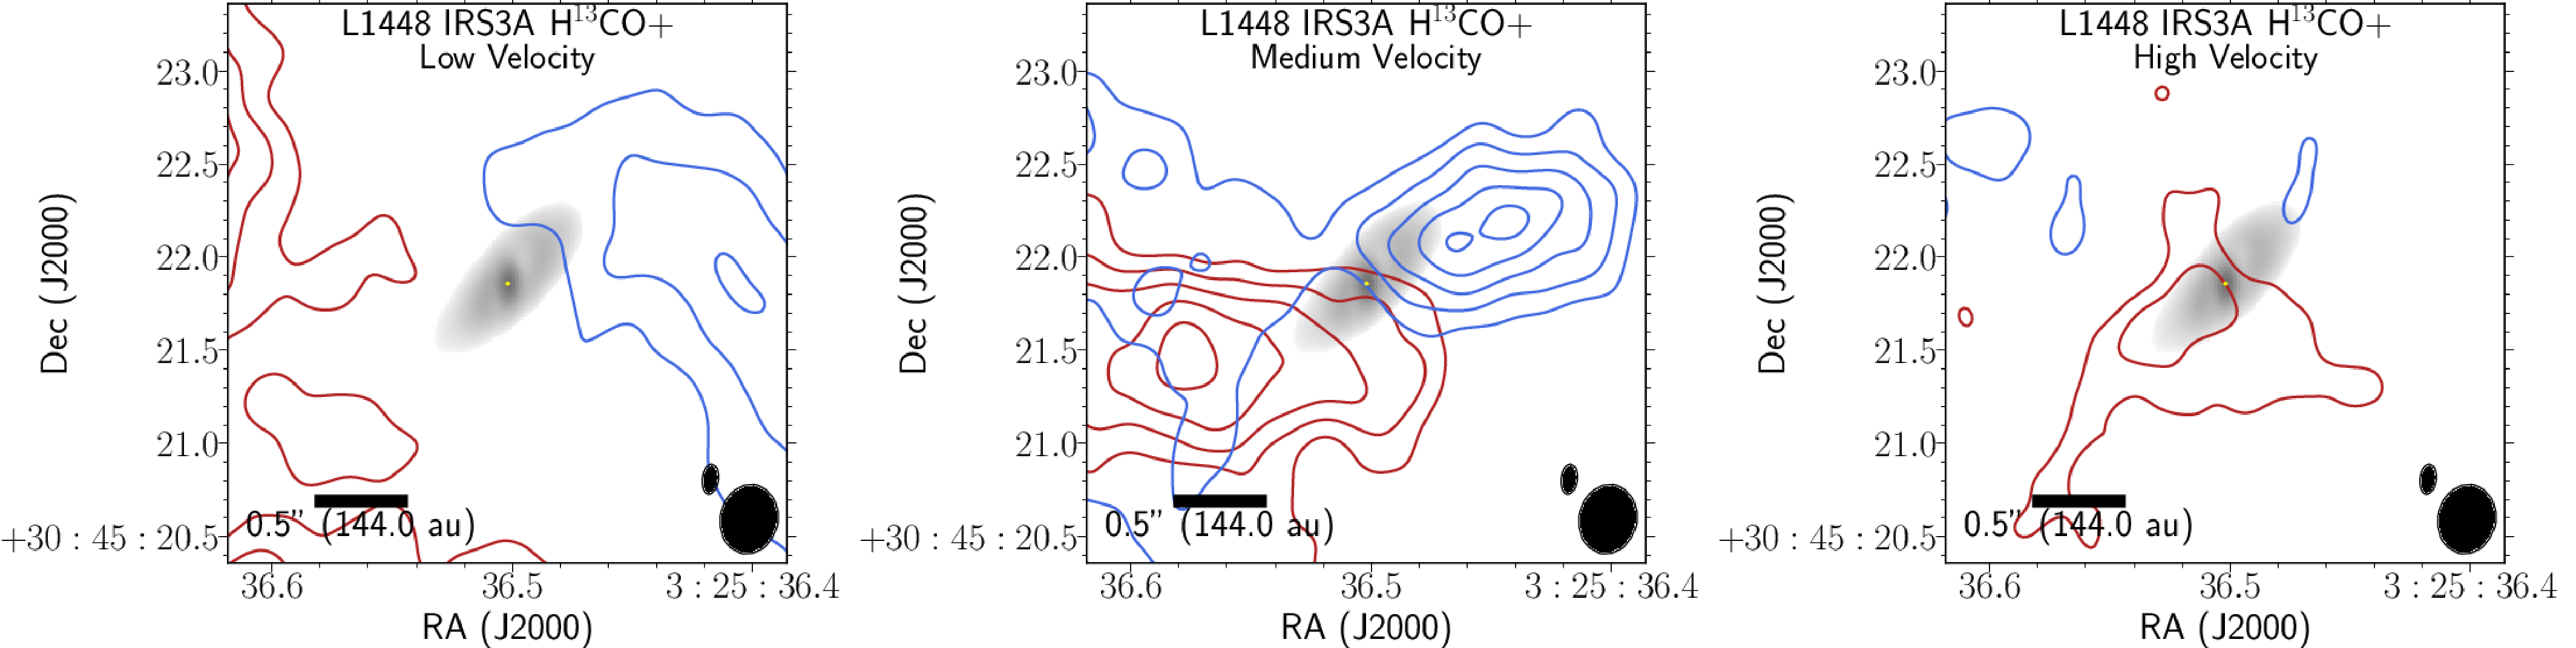
\includegraphics[width=1\textwidth]{img/L1448IRS3B_H13COp_image_taper400k__binned_panel.pdf} % h13cn
\end{center}
   \caption{\htcop\space integrated intensity map towards IRS3A generated at a position angle of 125\deg; whose emission predominately traces the intermediate dense, gaseous material of the inner envelope. The image is tapered with a 400~k$\lambda$\space Gaussian to best reduce the amount of noise and show the proper resolution to the spatial scales shown. The \htcop\space emission might trace a velocity gradient across the source, but \replaced{the compactness of the source}{the lack of strong emission coming from the disk itself} hinders resolving the kinematics. The columns correspond to low, medium, and high velocity ranges which are delineated as red(blue), respectively. \textbf{Low Velocity:} velocity ranges 5.2$\rightarrow$6.5~\kms (4.1$\rightarrow$5.2~\kms), contours start at 5(5)$\sigma$ and iterate by 2(2)$\sigma$ with the 1$\sigma$~level starting at 0.004(0.007)~Jy~beam$^{-1}$ for the red(blue) channels respectively. \textbf{Medium Velocity:}  velocity ranges 6.5$\rightarrow$7.4~\kms (3.0$\rightarrow$4.1~\kms), contours start at 3(3)$\sigma$ and iterate by 2(2)$\sigma$ with the 1$\sigma$~level starting at 0.003(0.003)~Jy~beam$^{-1}$ for the red (blue) channels respectively. \textbf{High Velocity:} velocity ranges 7.4$\rightarrow$8.6~\kms (1.8$\rightarrow$3.0~\kms), contours start at 3(3)$\sigma$ and iterate by 2(2)$\sigma$ with the 1$\sigma$~level starting at 0.002(0.0025)~Jy~beam$^{-1}$ for the red(blue) channels respectively. The \htcop\space synthesized beam (\htcopbeam) is the bottom-right most ellipse on each of the panels and the continuum synthesized beam (\contbeam) is offset diagonally.}\label{fig:irs3ah13copmoment}
\end{figure}


% Figure 6
\begin{figure}[H]
\begin{center}
   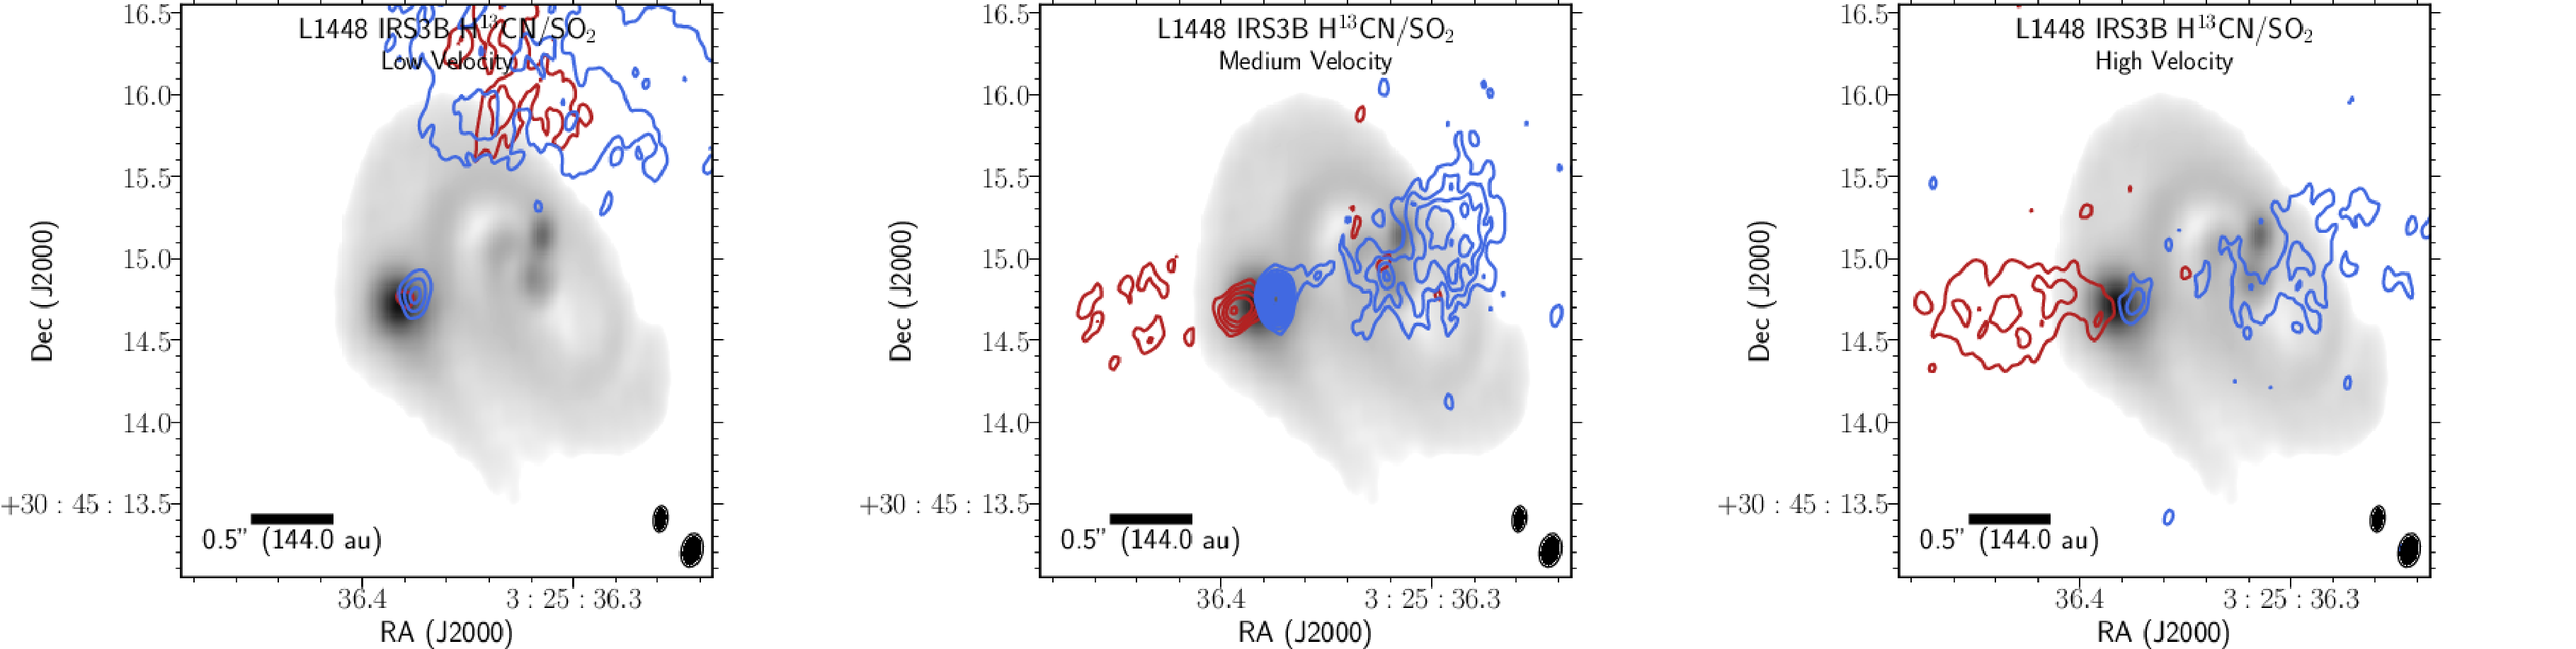
\includegraphics[width=1\textwidth]{img/L1448IRS3B_H13CN_clean_image_2_binned__panel.pdf} % h13cn
\end{center}
   \caption{\htcn/\sot\space integrated intensity map towards IRS3B, appears to trace near the outflow launch location from the tertiary, IRS3B-c. There is pretty large asymmetry in the velocity channels covered by the red and blue-shifted emission. The panels correspond to low, medium, and high velocity ranges which are delineated as red(blue), respectively. \textbf{Low Velocity:} velocity ranges 5.2$\rightarrow$7.2~\kms (4$\rightarrow$4.8~\kms), contours start at 5(5)$\sigma$ and iterate by 2(5)$\sigma$ with the 1$\sigma$~level starting at 0.0025(0.0021)~Jy~beam$^{-1}$ for the red(blue) channels respectively. \textbf{Medium Velocity:} velocity ranges 7.2$\rightarrow$9.2~\kms (3.2$\rightarrow$4~\kms), contours start at 5(5)$\sigma$ and iterate by 2(2)$\sigma$ with the 1$\sigma$~level starting at 0.0016(0.0016)~Jy~beam$^{-1}$ for the red(blue) channels respectively. \textbf{High Velocity:} velocity ranges 9.2$\rightarrow$11.2~\kms (1.6$\rightarrow$3.2~\kms), contours start at 4(4)$\sigma$ and iterate by 3(3)$\sigma$ with the 1$\sigma$~level starting at 0.0021(0.0021)~Jy~beam$^{-1}$ for the red(blue) channels respectively. The \htcn\space synthesized beam (\htcnbeam) is the bottom-right most ellipse on each of the panels and the continuum synthesized beam (\contbeam) is offset diagonally.}\label{fig:irs3bh13cnmoment}
\end{figure}






% Figure 9
\begin{figure}[H]
\begin{center}
   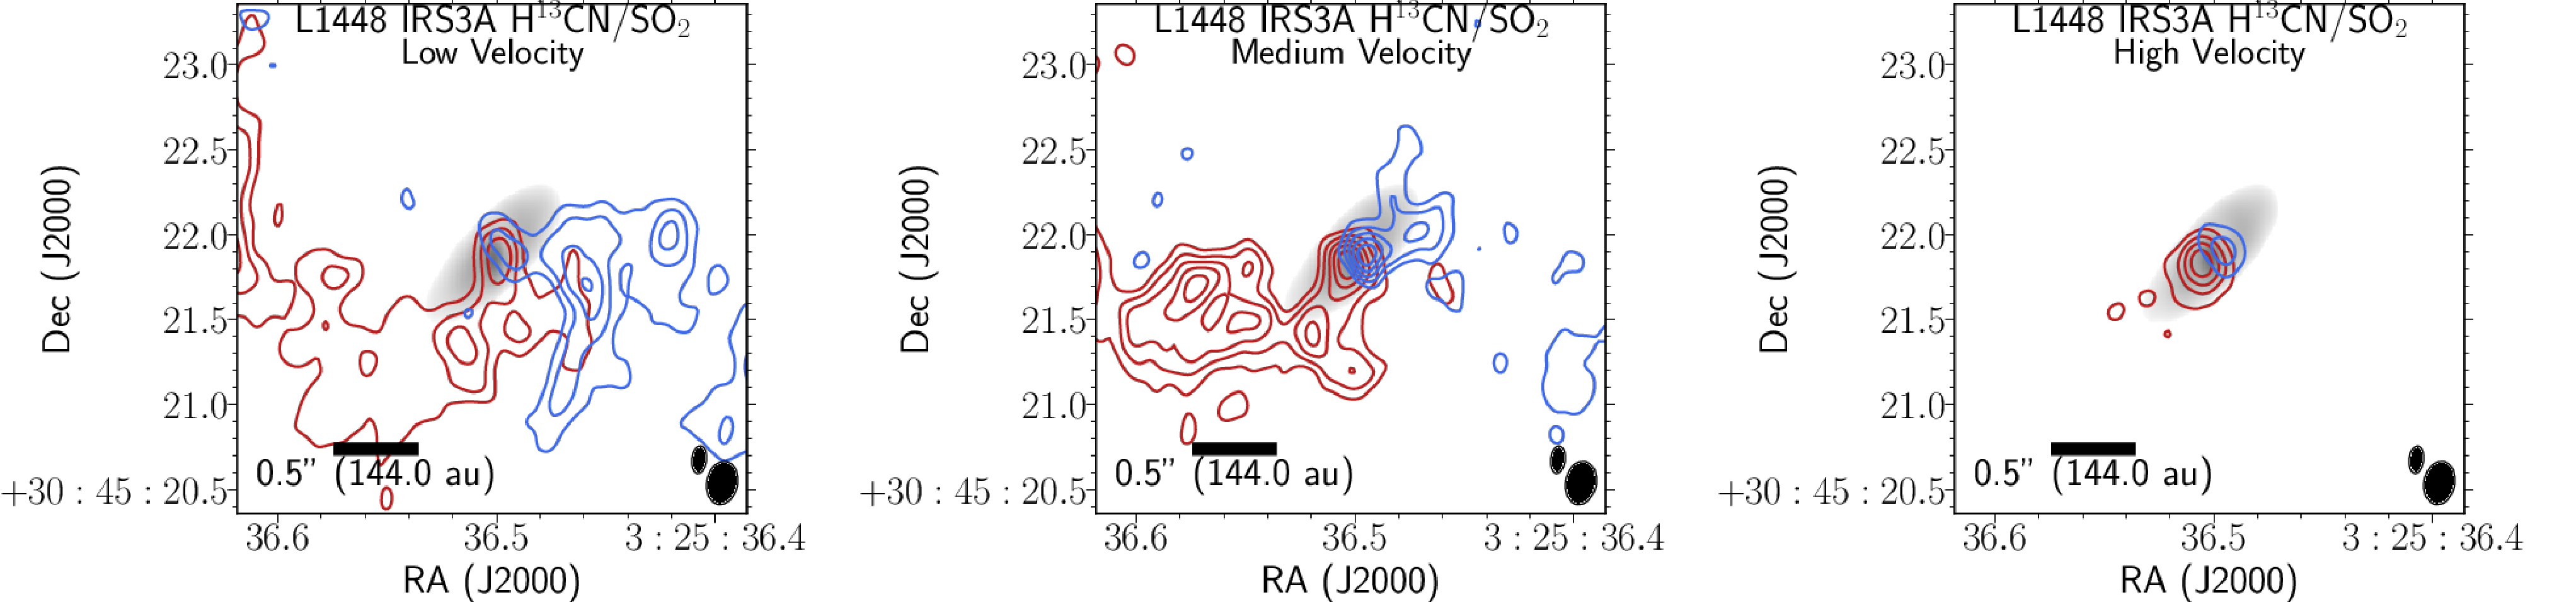
\includegraphics[width=1\textwidth]{img/L1448IRS3B_H13CN_image_taper1000k__-irs3apanel_irs3a.pdf} % h13cn
\end{center}
   \caption{\htcn/\sot\space integrated intensity map towards IRS3A; whose emission appears to trace rotation within the inner disk. The panels correspond to low, medium, and high velocity ranges which are delineated as red(blue), respectively. The system velocity of the \htcn/\sot\space emission (\ab5.4~km~s$^{-1}$) agrees with system velocity of \cso\space, likely tracing \htcn\space emission and not \sot\space emission. \textbf{Low Velocity:} velocity ranges 5.2$\rightarrow$6.5~\kms (4.1$\rightarrow$5.2~\kms), contours start at 4(4)$\sigma$ and iterate by 2(2)$\sigma$ with the 1$\sigma$~level starting at 0.0021(0.0021)~Jy~beam$^{-1}$ for the red(blue) channels respectively. \textbf{Medium Velocity:}  velocity ranges 6.5$\rightarrow$7.4~\kms (3.0$\rightarrow$4.1~\kms), contours start at 4(4)$\sigma$ and iterate by 2(2)$\sigma$ with the 1$\sigma$~level starting at 0.0016(0.0016)~Jy~beam$^{-1}$ for the red (blue) channels respectively. \textbf{High Velocity:} velocity ranges 7.4$\rightarrow$8.6~\kms (1.8$\rightarrow$3.0~\kms), contours start at 4(4)$\sigma$ and iterate by 3(3)$\sigma$ with the 1$\sigma$~level starting at 0.0021(0.0021)~Jy~beam$^{-1}$ for the red(blue) channels respectively. The \htcn\space synthesized beam (\htcnbeam) is the bottom-right most ellipse on each of the panels and the continuum synthesized beam (\contbeam) is offset diagonally.}\label{fig:irs3ah13cnmoment}
\end{figure}



% figure will go here for pv cutout, 2 of them







% Figure 10
\begin{figure}[H]
\begin{center}
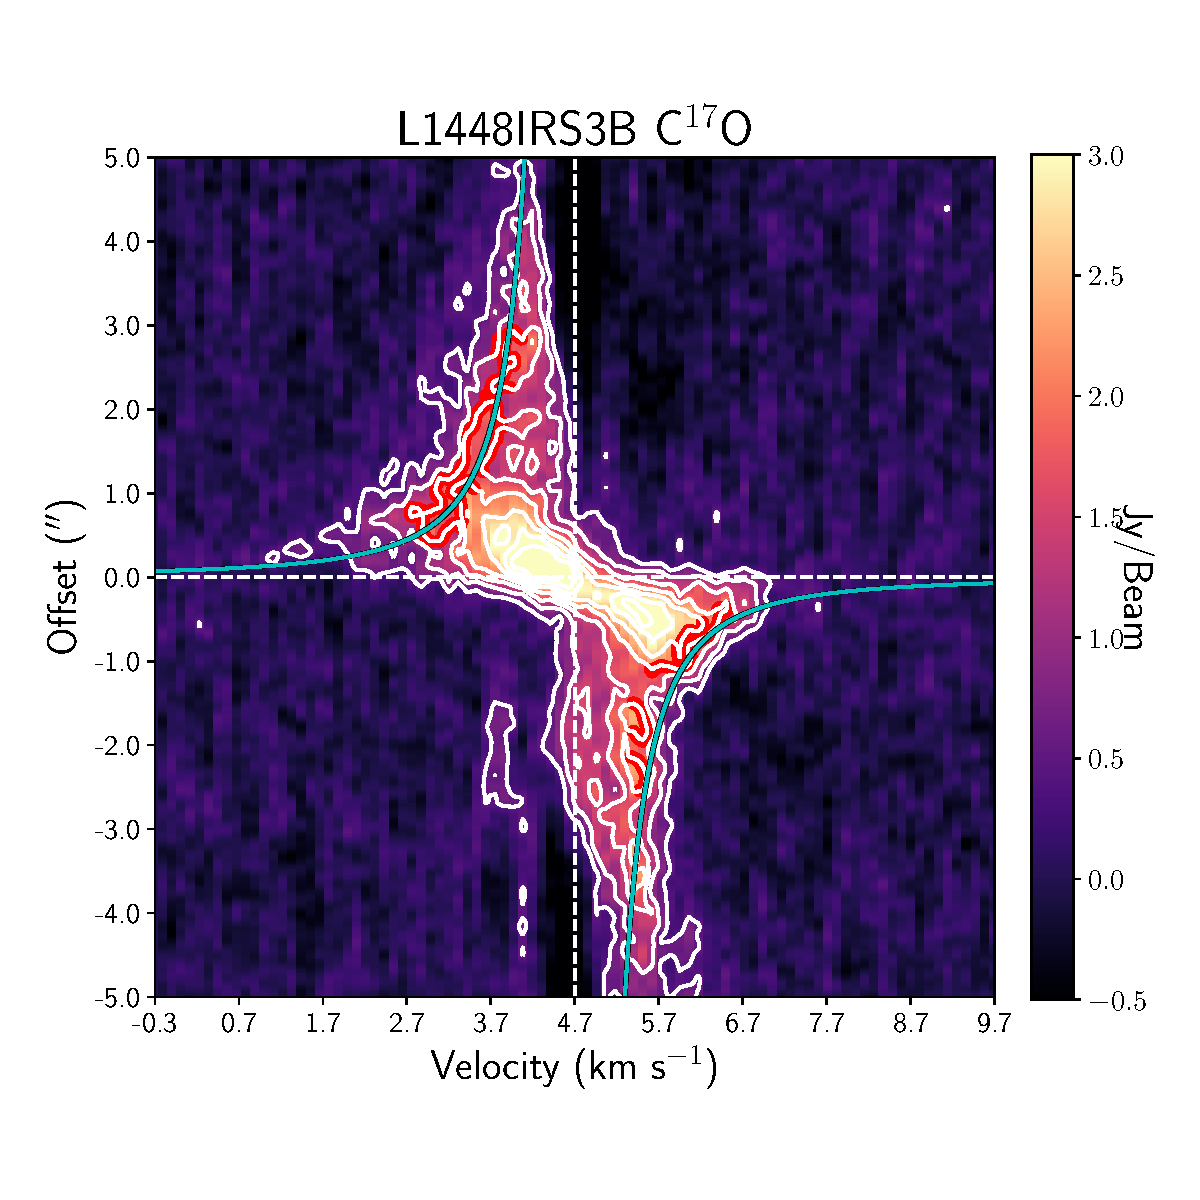
\includegraphics[width=0.44\textwidth]{img/irs3b_c17o_pv.pdf}
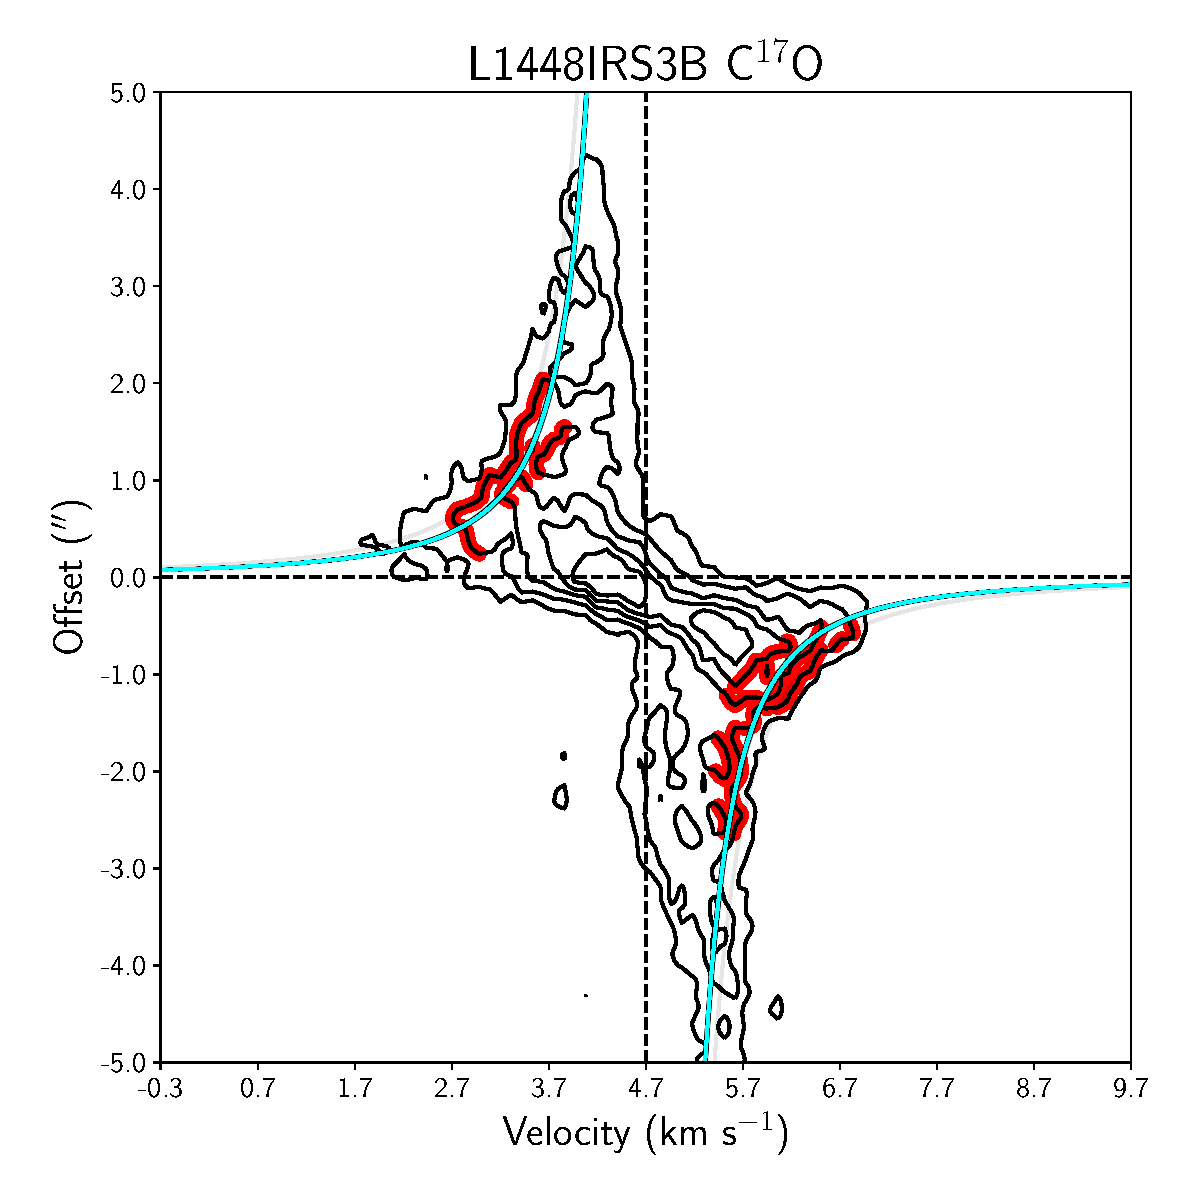
\includegraphics[width=0.44\textwidth]{img/PV-Diagram_L1448IRS3B_C17O_image_taper1500k_fit_xtr.pdf}
\end{center}
\caption{PV-diagrams of IRS3B \cso\space emission generated at a position angle of 29\deg, with the cyan lines corresponding to the fit of 1.15~\solm, demonstrating the data could be reproduced reasonably well with a Keplerian disk orbiting a 1.15~\solm\space protostar. The cyan line traces the median fit for numeric Keplerian orbital fit routine while the black lines represent 100 randomly sampled MCMC fits, used to estimate errors. As evident, this methodology selectively fits the highest velocity emission that is symmetric in the protostellar system. The white/black contours trace regions starting from 3$\sigma$ at 2$\sigma$\space intervals, where $\sigma\approx$0.14~Jy~beam$^{-1}$. The red contours trace the regions selected for the MCMC fit which are defined as the 10 and 12$\sigma$\space levels as to not fit the diffuse large-scale emission.}\label{fig:l1448irs3b_c17o_pv}
\end{figure}








\begin{figure}[H]
\begin{center}
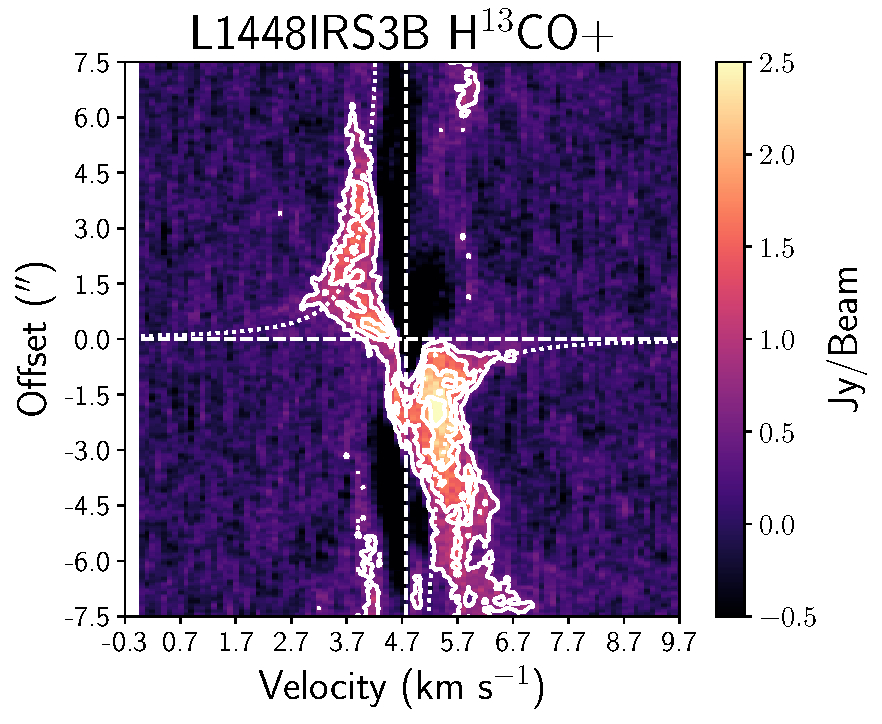
\includegraphics[width=0.5\textwidth]{img/PV-Diagram_L1448IRS3B_H13COp_image_taper1500k.pdf}
\end{center}
\caption{\htcop\space emission towards IRS3B generated at a position angle of 29\deg, with the white dashed lines corresponding to the Keplerian fit of 1.15~\solm\space from the fit to \cso, demonstrating the data are not inconsistent with a 1.15~\solm\space protostar, similarly demonstrated from the \cso\space emission Keplerian fits. The PV diagram shows a large amount of asymmetry in the molecular line emission close to system velocity, with emission  at velocities in  excess of Keplerian particularly at the red-shifted velocities. These are possible indications of infalling material from the envelope given the spatial location this emission. The white contours trace regions starting from 3$\sigma$ at 2$\sigma$\space intervals, where $\sigma\approx$0.15~Jy}\label{fig:l1448irs3b_h13cop_pv}
\end{figure}






% Figure 15
\begin{figure}[H]
\begin{center}
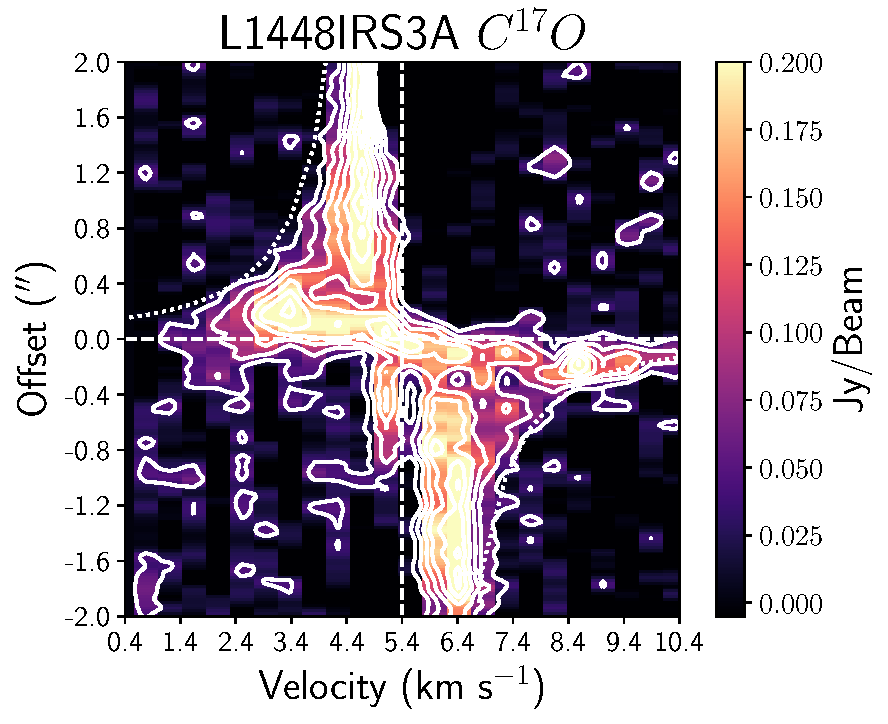
\includegraphics[width=0.44\textwidth]{img/PV-Diagram_L1448IRS3B_C17O_clean_binnedwide.pdf}
\end{center}
\caption{Position-velocity diagrams of IRS3A \cso\space emission generated at a position angle of 125\deg, with the dotted lines corresponding to 1.4~\solm. The emission suffers from the lower spatial sampling across the source and the extended, resolved-out emission from the IRS3B$+$A envelope/core. Similarly, strong spatial integration (width of slice 0\farcs3) restrictions were placed when making the PV diagram to limit the inclusion of large-scale emission. \deleted{Further constraints on the viewing distance (0\farcs5 displacement from the source center) were placed to help avoid the large scale emission.}}\label{fig:l1448irs3a_cso_pv}
\end{figure}








% Figure 14
\begin{figure}[H]
\begin{center}
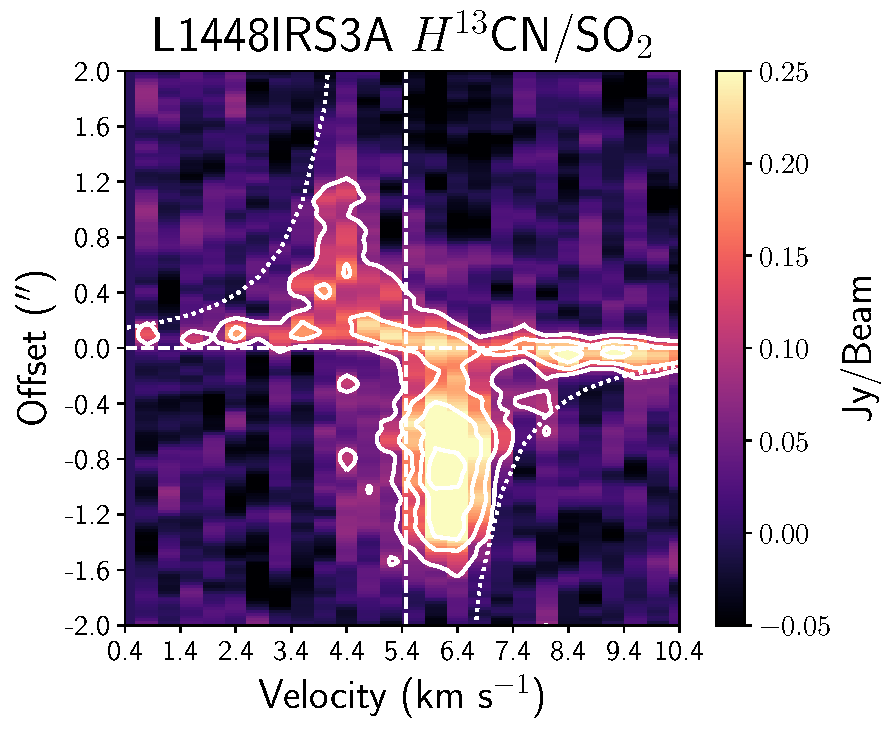
\includegraphics[width=0.44\textwidth]{img/irs3a_h13cn_pv.pdf}
\end{center}
\caption{Position-velocity diagram of IRS3A \htcn/\sot\space emission with the dotted lines corresponding to Keplerian velocities for a 1.4~\solm\space protostar. This PV diagram places a constraint on the possible protostellar mass parameter of \ab1.4~\solm. The IRS3A mass is less well constrained due to the compactness of the emission. Strong spatial integration (width of slice 0\farcs3) restrictions were placed when making the PV diagram to help limit the inclusion of large scale emission. Further constraints on the viewing distance (0\farcs5 displacement from the source center) were placed to help limit contributions from the large scale emission.}\label{fig:l1448irs3a_h13cn_pv}
\end{figure}
% Figure 12


% Figure 9
\begin{figure}[H]
\begin{center}
   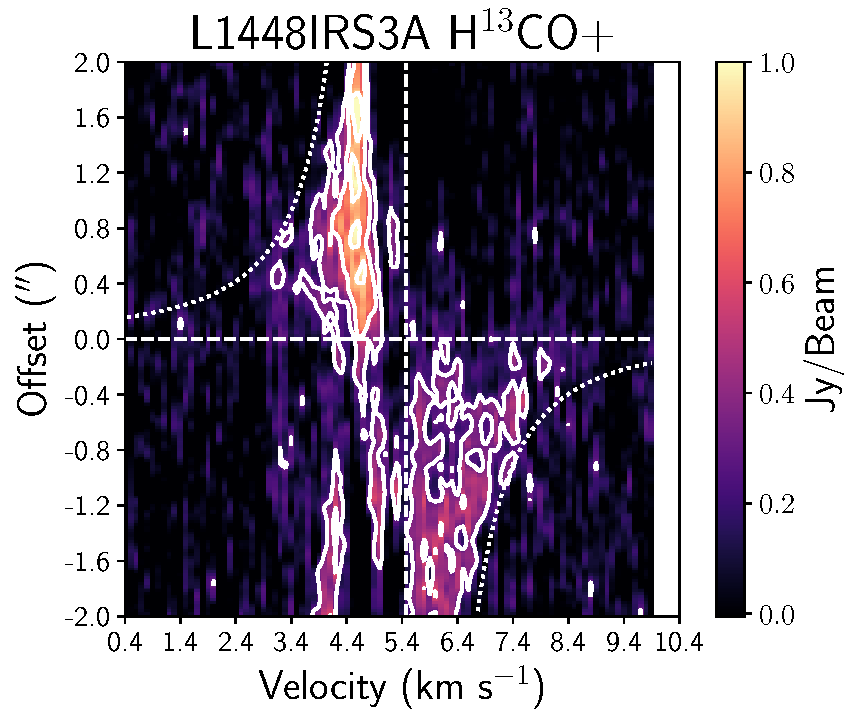
\includegraphics[width=0.44\textwidth]{img/PV-Diagram_L1448IRS3B_H13COp_image_taper1500k-wide.pdf} % h13cn
\end{center}
   \caption{Position-velocity diagram of IRS3A \htcop\space  generated at a position angle of 125\deg; whose emission predominately traces the intermediate dense, gaseous material of the inner envelope. The emission suffers lower spatial sampling across the source and less emission \replaced{is present towards the source}{is coming from the disk}. The dotted line corresponds to a central protostellar mass of 1.4~\solm.}\label{fig:l1448irs3a_h13cop_pv}
\end{figure}




% Figure 7
\begin{figure}[H]
\begin{center}
   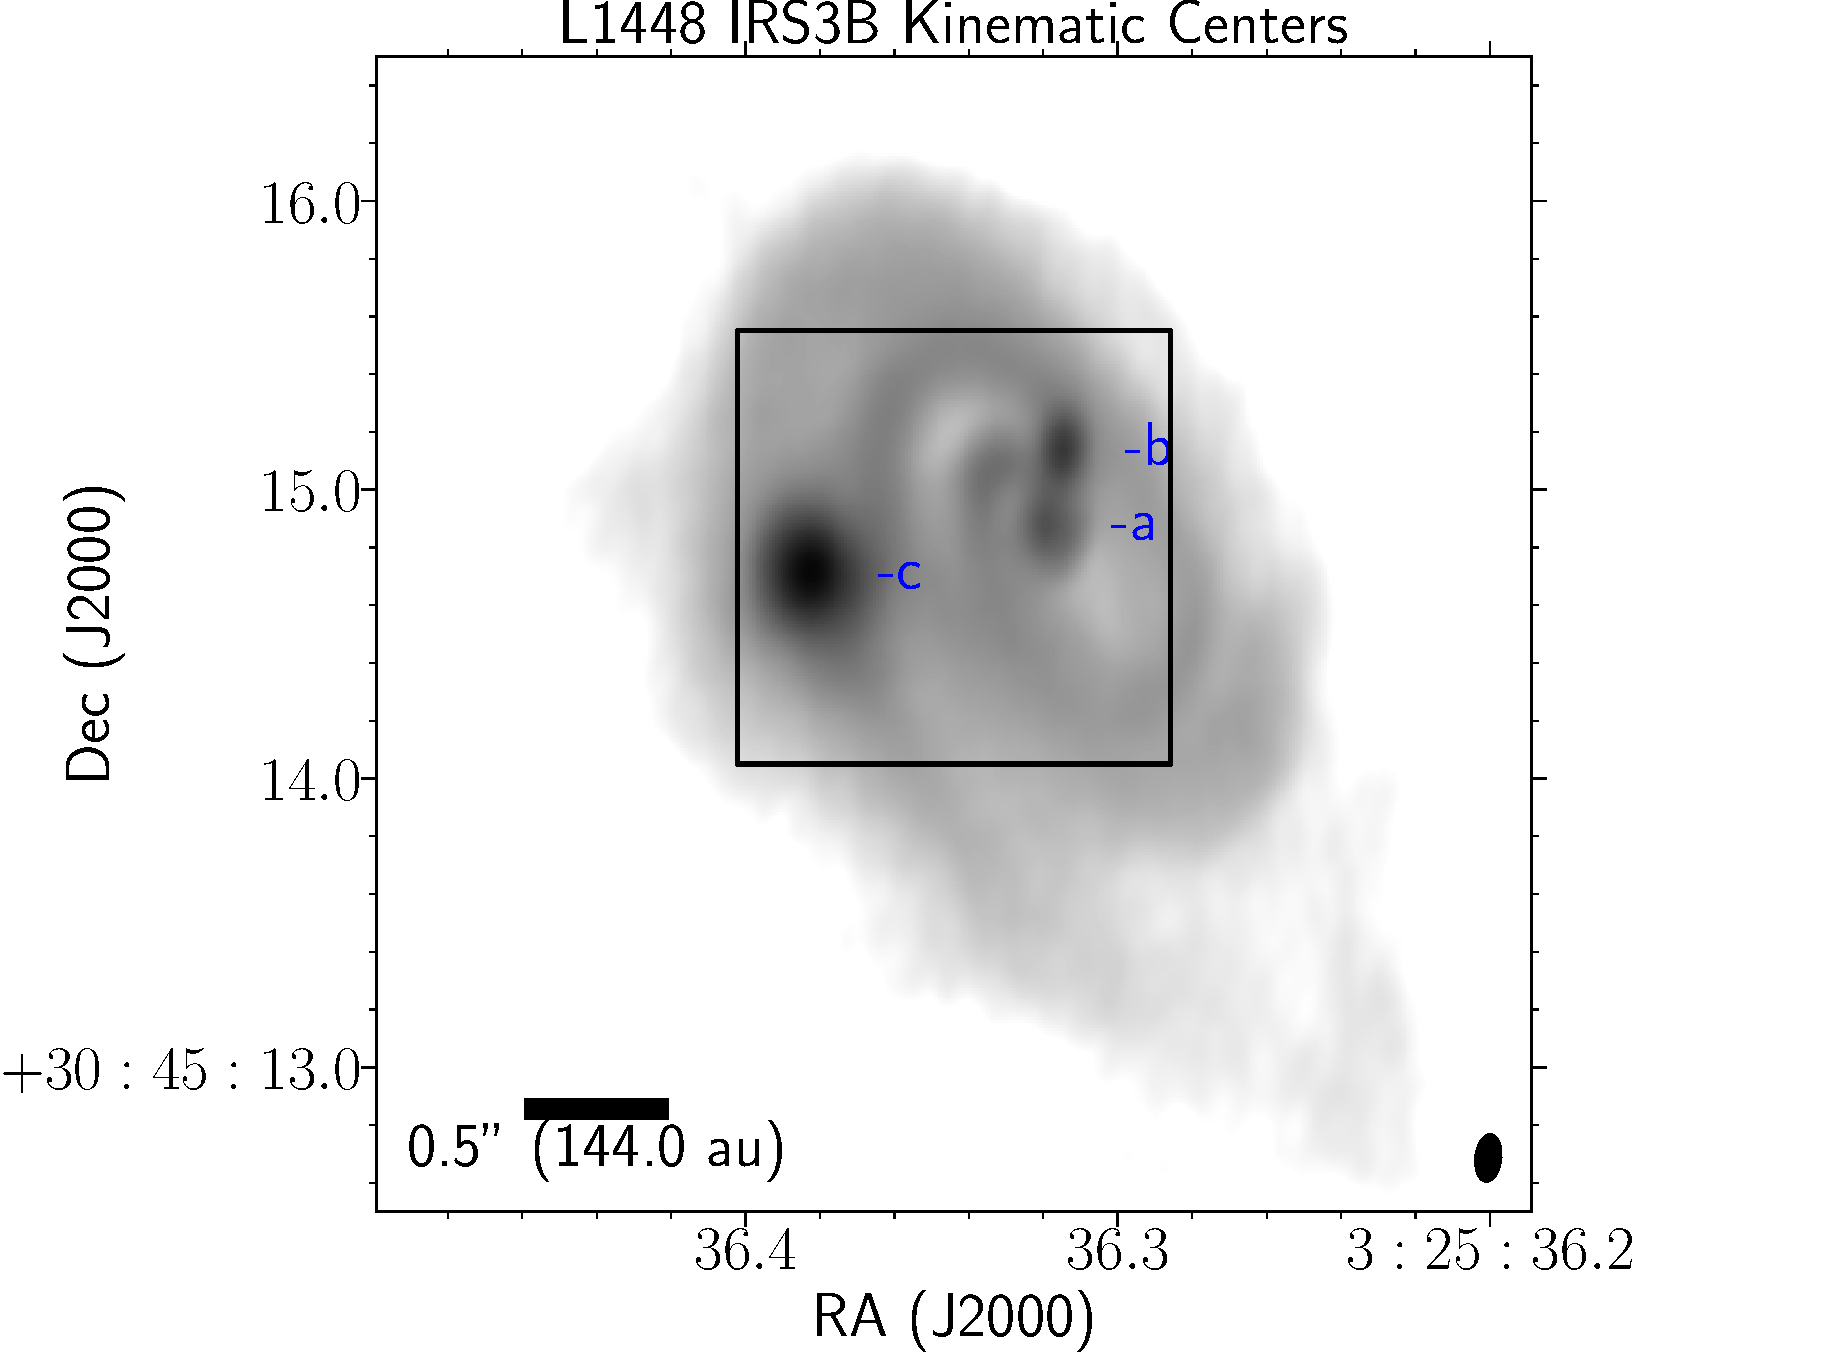
\includegraphics[width=0.48\textwidth]{img/L1448IRS3B_cont_robust05kincenters.pdf} % h13cn
   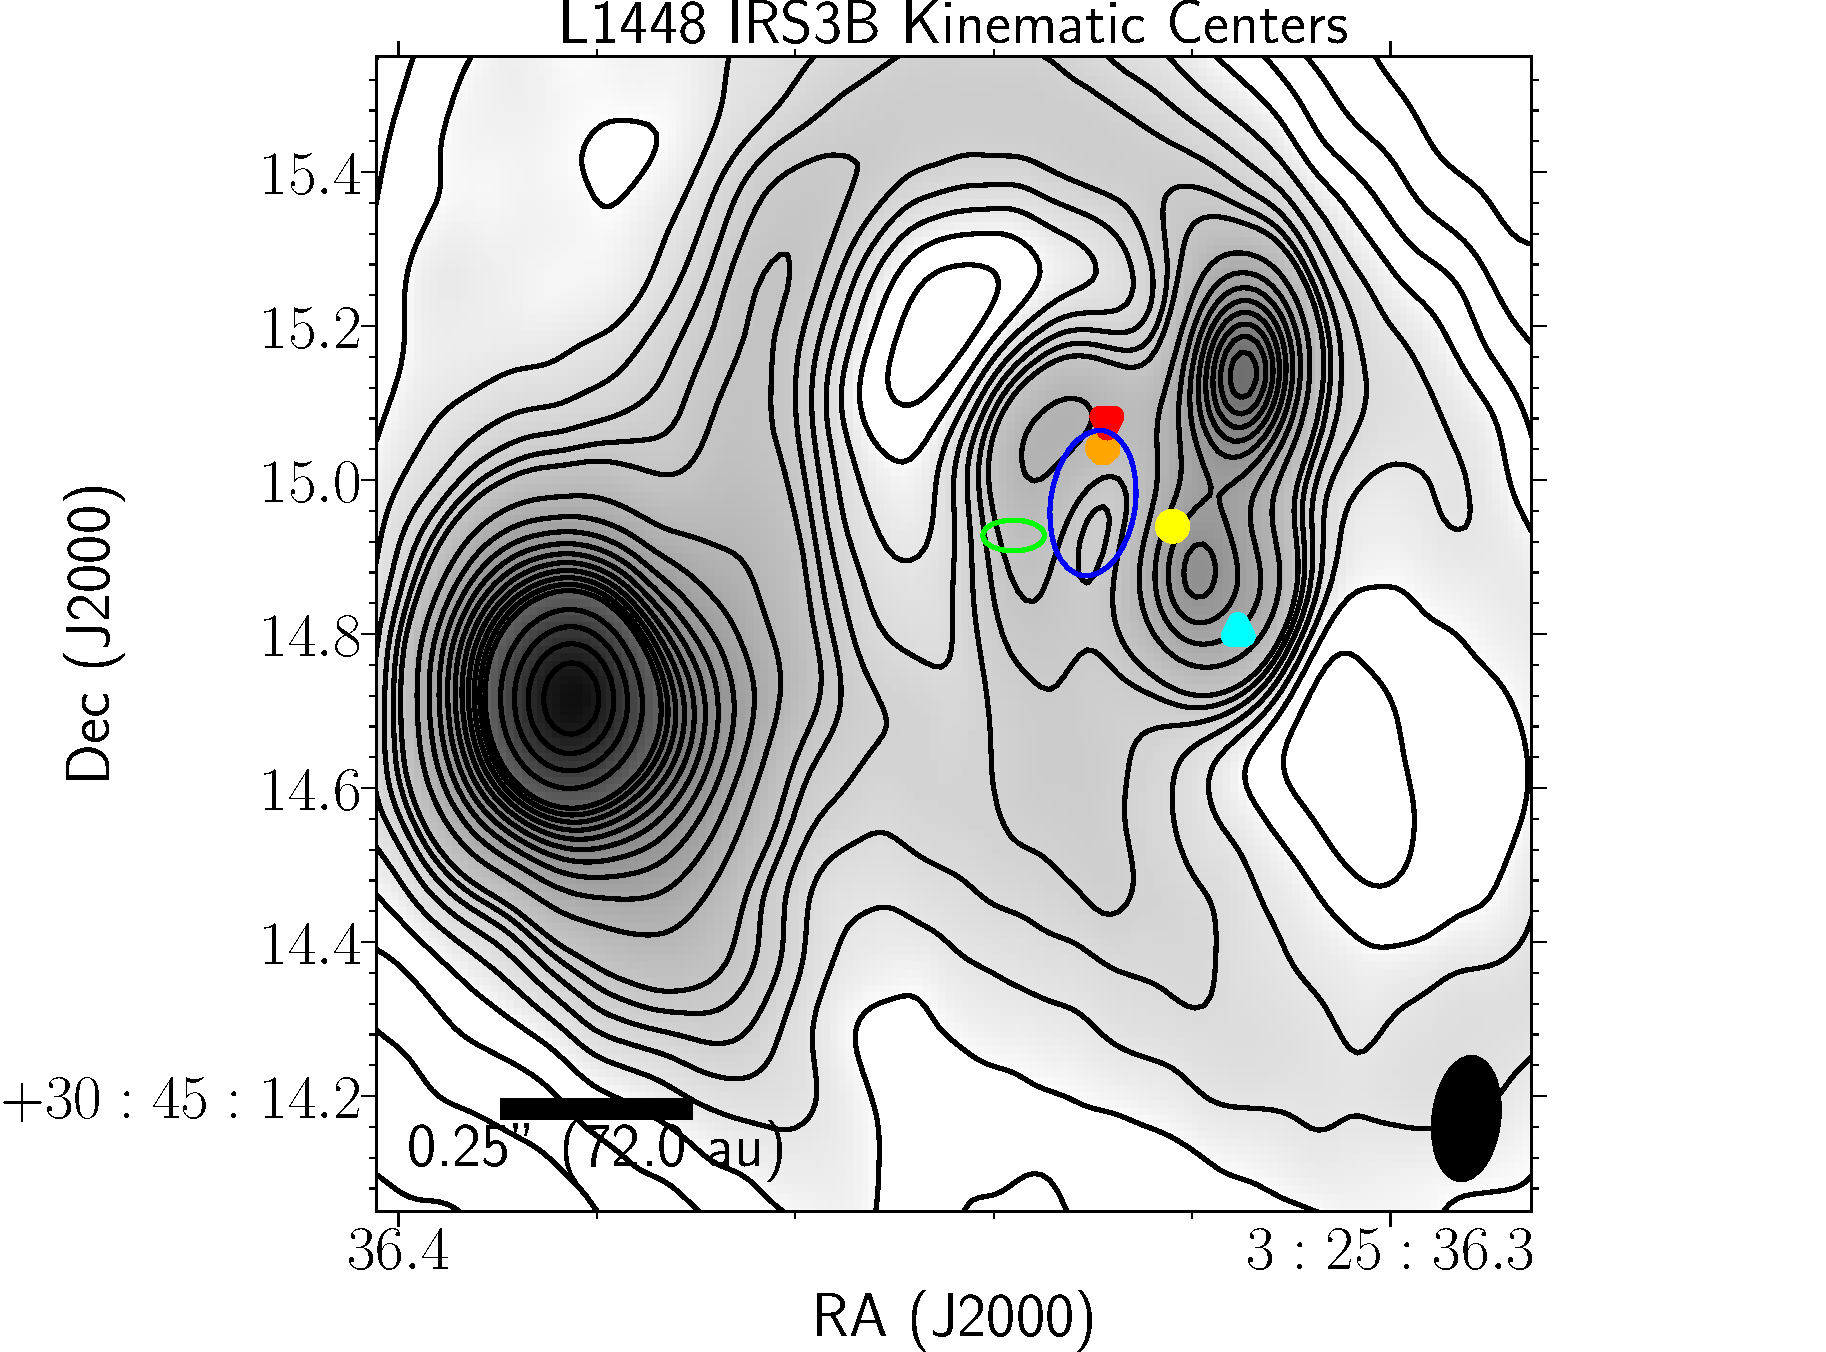
\includegraphics[width=0.48\textwidth]{img/L1448IRS3B_cont_robust05kincenters_zoom.pdf} % h13cn
\end{center}
   \caption{Positions of the various ``kinematic centers'' that have been fit from \cso\space emission at IRS3B in relation to continuum structure. The grayscale is the dust continuum from Figure~\ref{fig:contimage}. Left: The red colored texts detail the locations of continuum sources, presumed to be protostars. Right: A zoom in on the region indicated by the black rectangle in the left image. The red and blue triangles indicate the central Gaussian fit of the highest Doppler-shifted velocity emission with the yellow circle indicating the midpoint. The orange circle indicates the center that best constructs the PV diagram symmetrically. The green ellipse is the model Keplerian centroid fit with the respective error as indicated by the size of the ellipse (see Section~\ref{sec:kmodelresults}). The blue ellipse is the \cso\space beam (\csobeam) centered on the region of emission deficit for size comparison. The contours start at 10$\sigma$\space and iterate by 10$\sigma$\space with the 1$\sigma$~level starting at 8.5$\times10^{-5}$~Jy~beam$^{-1}$. The region of deficit, first identified in Figure~\ref{fig:zoomincont}\space is shown to be centered within the three various kinematic center fits and are marginally separated by less than a few beams.}\label{fig:kincenter}
\end{figure}



% Figure 13
\begin{figure}[H]
\begin{center}
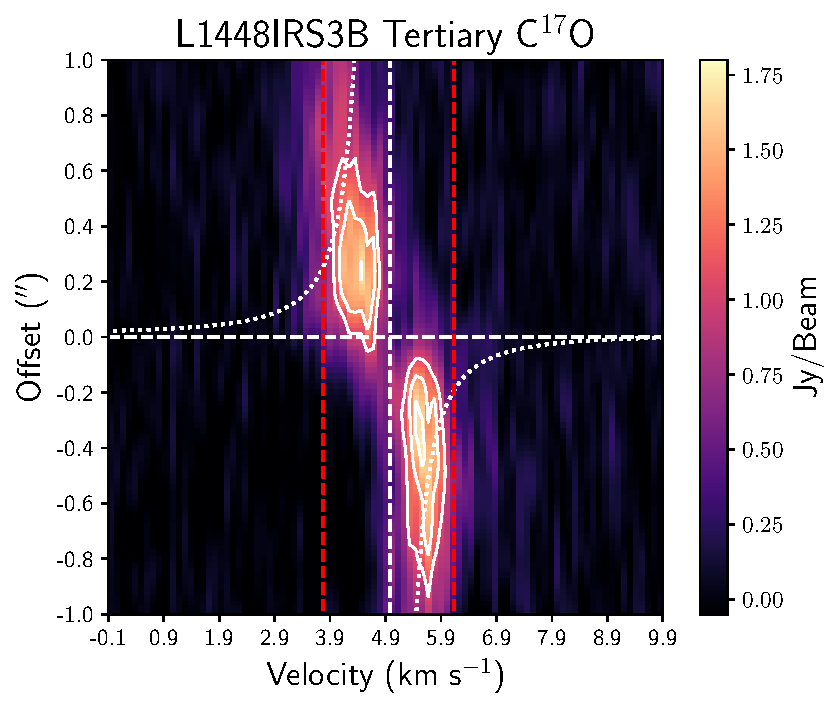
\includegraphics[width=0.5\textwidth]{img/PV-Diagram_L1448IRS3B_C17O_image_taper1500k_image_tertiary31.pdf}
\end{center}
\caption{PV-diagram of \cso\space toward IRS3B-c, the tertiary. The white lines corresponding to a Keplerian curve of a 0.2~\solm\space protostellar source. These fits place an upper limit to the mass of the tertiary companion to $<$0.2~\solm, since any larger mass and we would expect to see emission extending to high velocity, indicating the tertiary would be affecting disk kinematics. The red dashed lines indicate the maximum Keplerian velocities at the radius of IRS3B-c in the rotating disk corresponding to the 1.15~\solm\space mass of the central potential. Emission outside of these bounds could be due to the tertiary affecting disk kinematics, but from this analysis, we cannot detect an obvious effect of the tertiary on the disk kinematics. The white/black contours trace regions starting from 14$\sigma$ at 4$\sigma$\space intervals, where $\sigma\approx$0.1~Jy~beam$^{-1}$.}\label{fig:l1448irs3b_c17o_pv_tert}
\end{figure}
% Figure 16
\begin{figure}[H]
\begin{center}
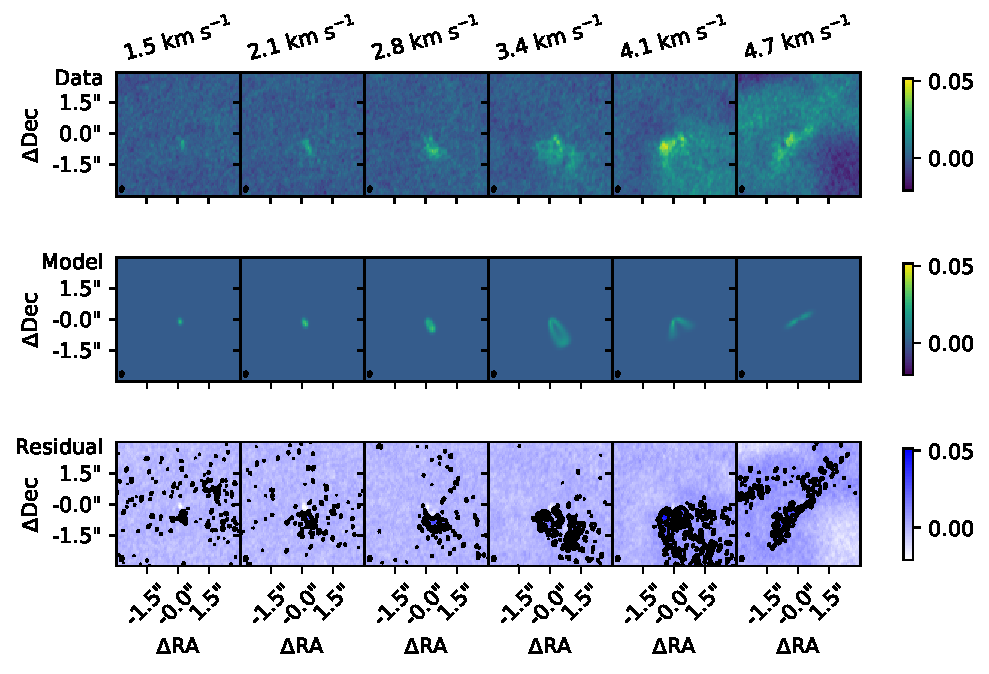
\includegraphics[width=0.5\textwidth]{img/Channelplot_irs3bplotblue_C17O.pdf}
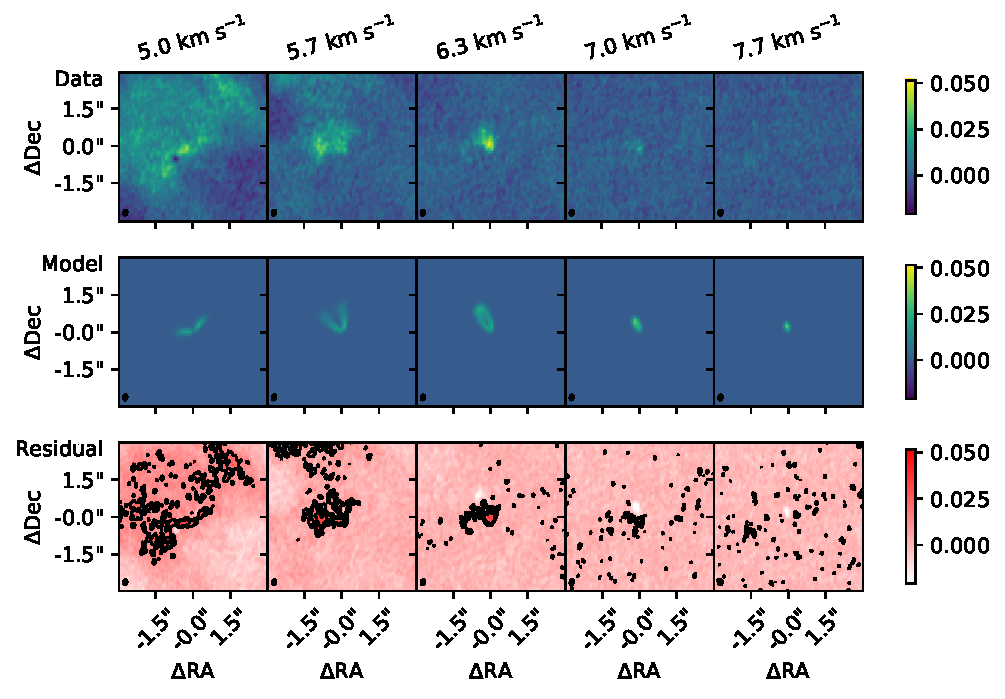
\includegraphics[width=0.5\textwidth]{img/Channelplot_irs3bplotred_C17O.pdf}
\end{center}
\caption{IRS3B Kinematic Model comparison: A representative selection of channel maps that demonstrate the fit of the model to the data. The top figure is the blue Doppler shifted emission while the bottom figure is the red Doppler shifted emission. The first row contours are the model contours, generated at the 2, 3, 5, and 10$\sigma$ level overlaid the data channels selected at the same velocity. The second row is the residual contours (2 and 3$\sigma$) overlaid the same data channels. System velocity is \ab4.8~km~s$^{-1}$. It should be noted the highly correlated structure visible in the residuals. This reflects an imperfect fit to the data given that the circumstellar disk itself is asymmetric.}\label{fig:c17o_res}
\end{figure}


% Figure 17
\begin{figure}[H]
\begin{center}
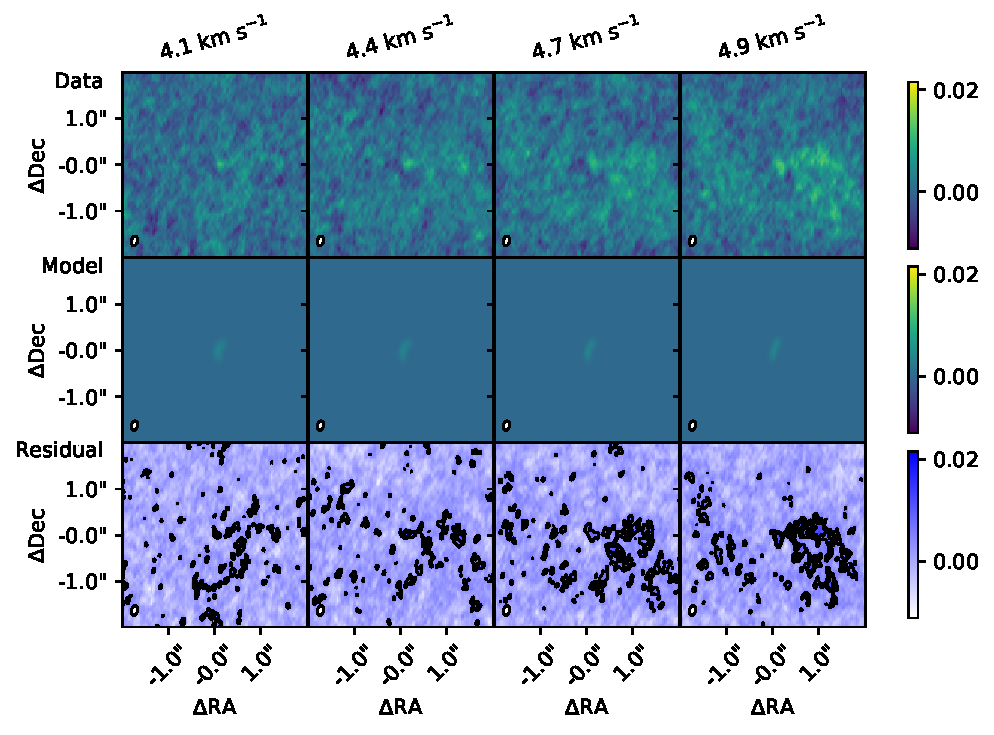
\includegraphics[width=0.5\textwidth]{img/Channelplot_h13cnplotblue_H13CN.pdf}
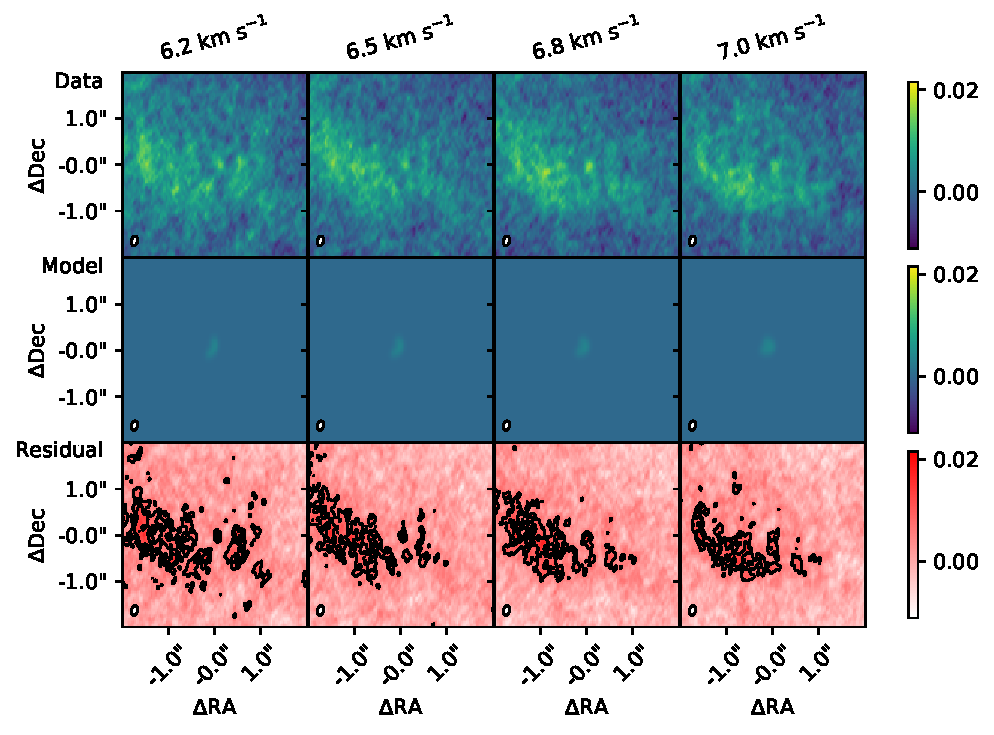
\includegraphics[width=0.5\textwidth]{img/Channelplot_h13cnplotred_H13CN.pdf}
\end{center}
\caption{IRS3A Kinematic Model comparison: A representative selection of channel maps that demonstrate the fit of the model to the data. The top figure is the blue Doppler shifted emission while the bottom figure is the red Doppler shifted emission. The first row contours are the model contours, generated at the 2, 3, 5, and 10$\sigma$  level overlaid the data channels selected at the same velocity to not overshadow the emission. The second row is the residual contours overlaid the same data channels. System velocity is \ab5.2~km~s$^{-1}$. There is residual emission at scales much larger than the continuum disk, especially prevalent near the system velocity, likely due to large scale emission from the cloud that is not included in the disk.}\label{fig:h13cn_res}
\end{figure}


% Figure 19
\begin{figure}[H]
\begin{center}
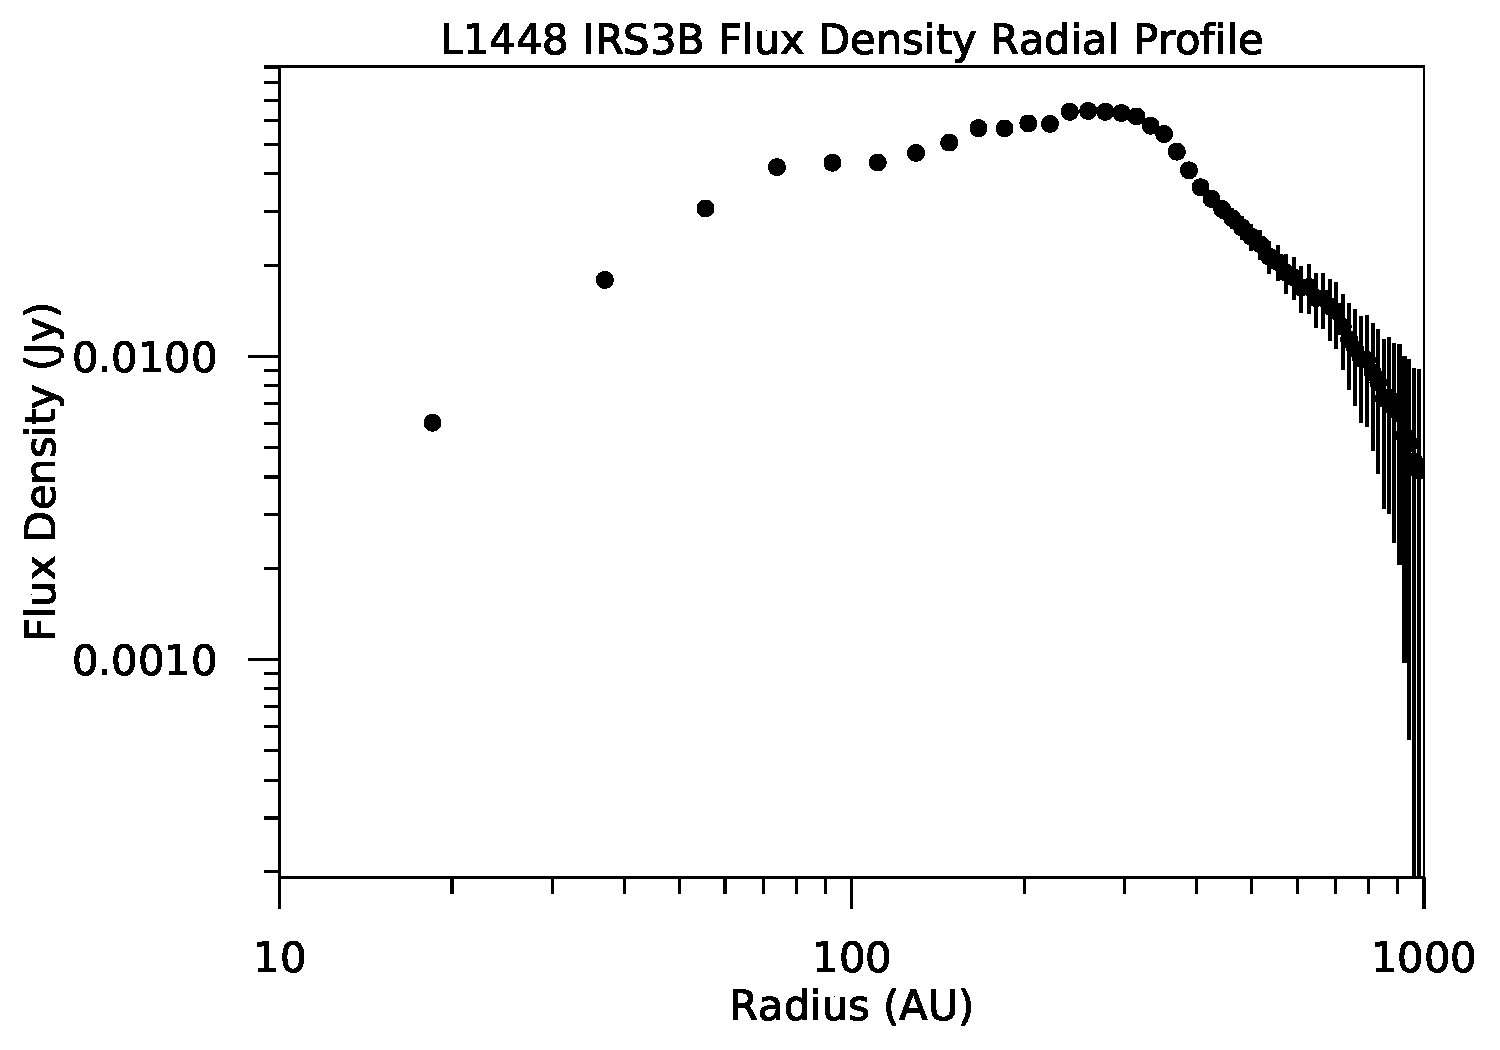
\includegraphics[width=0.49\textwidth]{img/L1448N-dgr-linear-intensity-c17o_cont.pdf}
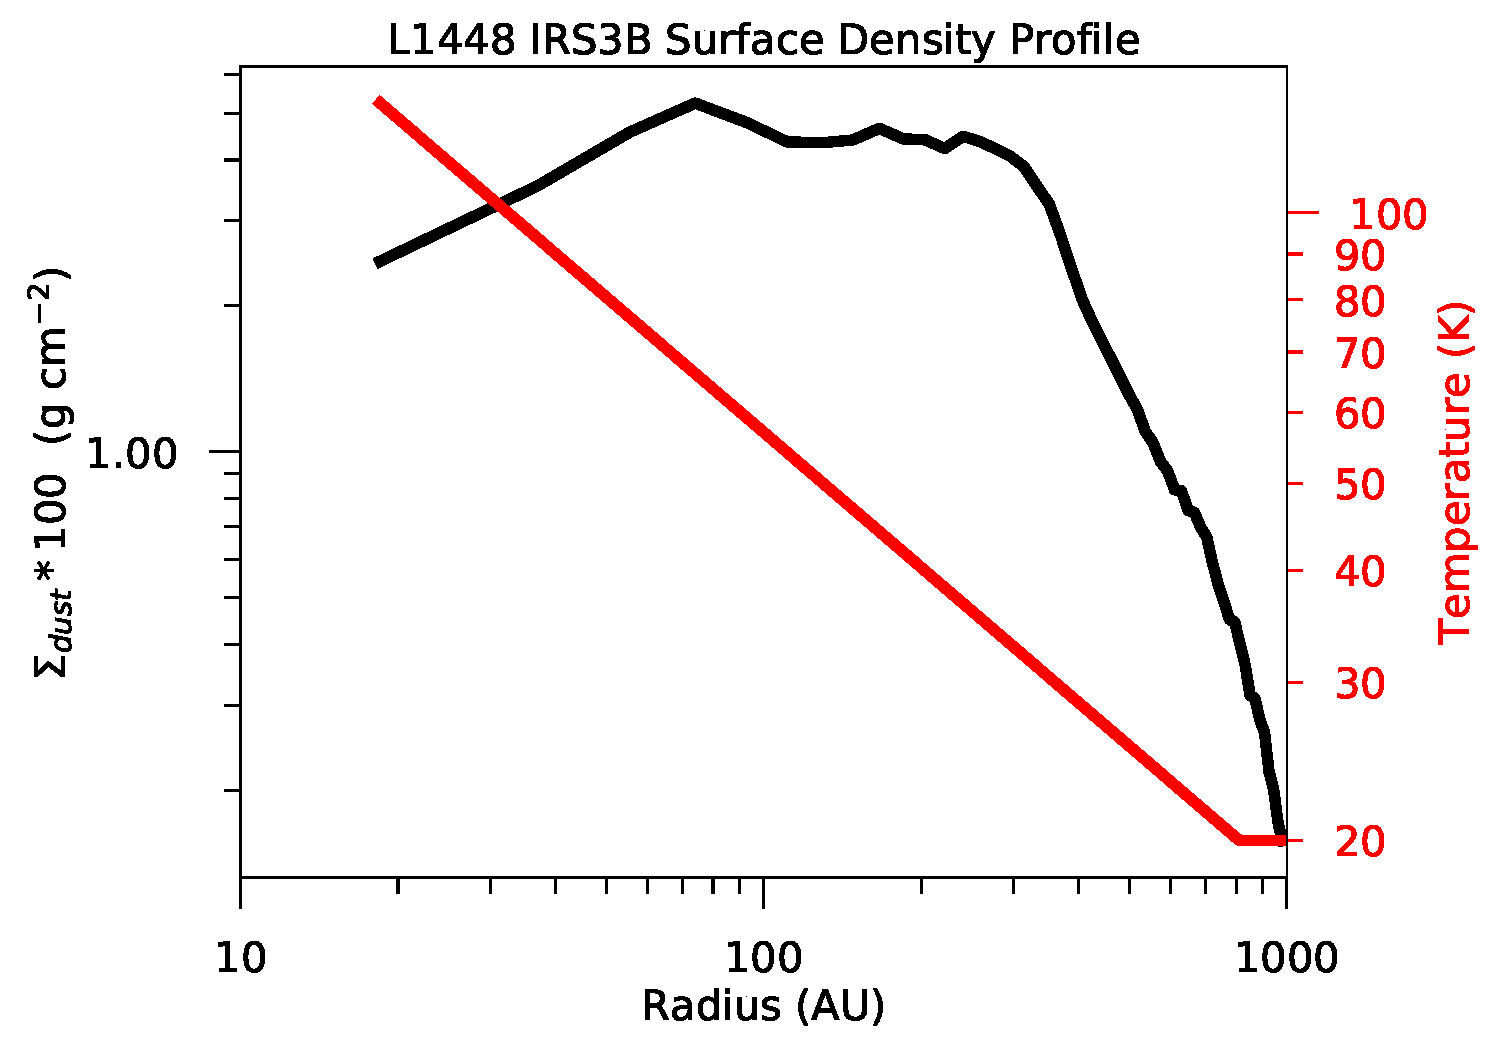
\includegraphics[width=0.49\textwidth]{img/L1448N-dustgas-surface-density-loglog.pdf}
\end{center}
\caption{The left plot is the continuum flux \added{density} radial profile of IRS3B. The right plot is the deprojected radial surface density profile of the dust continuum in black \deleted{points}, while the red line is the radial temperature profile of the disk. \replaced{The slope is -0.5 and the temperature is scaled such that the temperature of the disk}{The temperature profile is $\propto\text{R}^{-0.5}$ and is scaled such that} at 100~AU is described via (30~K)$\times(L_{*}$/\lsun)$^{0.25}\approx40.1$~K.}\label{fig:surfacedensity}
\end{figure}

% figure 20
\begin{figure}[H]
\begin{center}
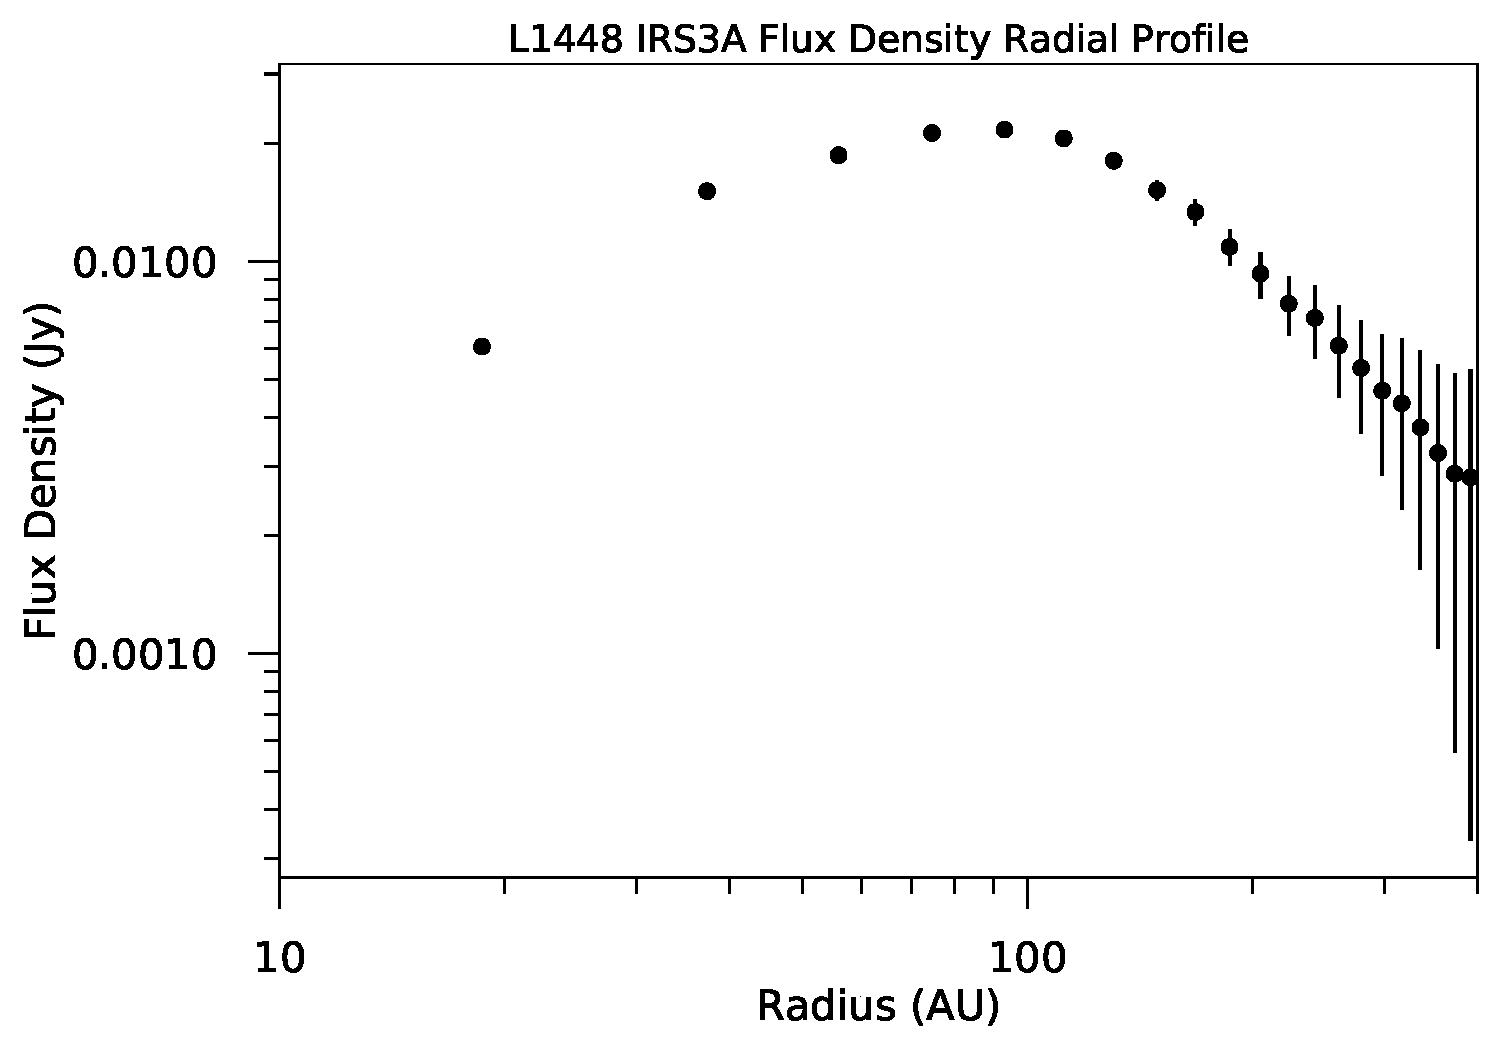
\includegraphics[width=0.49\textwidth]{img/L1448N-intensity-rad-xsec-cont_robust-05_wide.pdf}
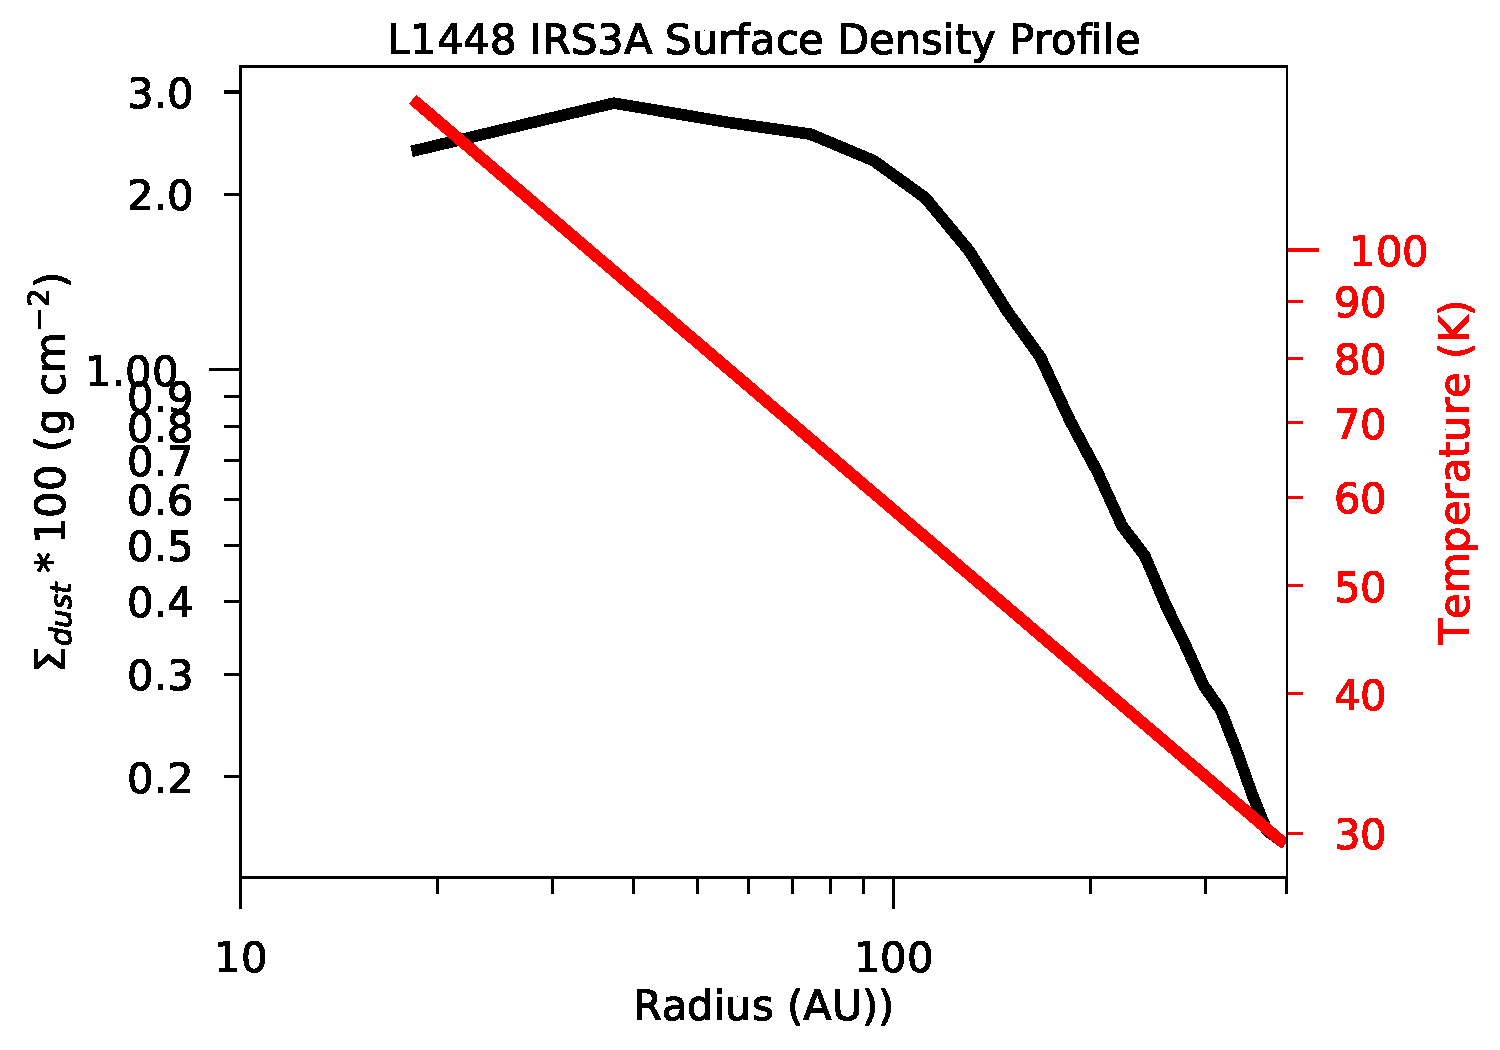
\includegraphics[width=0.49\textwidth]{img/L1448N-surface-density-lograd-xsec-cont_robust-05_wide.pdf}
\end{center}
\caption{The left plot is the continuum flux \added{density} radial profile of IRS3A. The right plot is the radial surface density profile of the dust continuum in black\deleted{points}, while the red line is the radial temperature profile of the disk. \replaced{The slope is -0.5 and the temperature is scaled such that the temperature of the disk}{The temperature profile is $\propto\text{R}^{-0.5}$ and is scaled such that} at 100~AU is described via (30~K)$\times(L_{*}$/\lsun)$^{0.25}\approx53.1$~K.}\label{fig:irs3asurfacedensity}
\end{figure}

% figure 21
\begin{figure}[H]
\begin{center}
%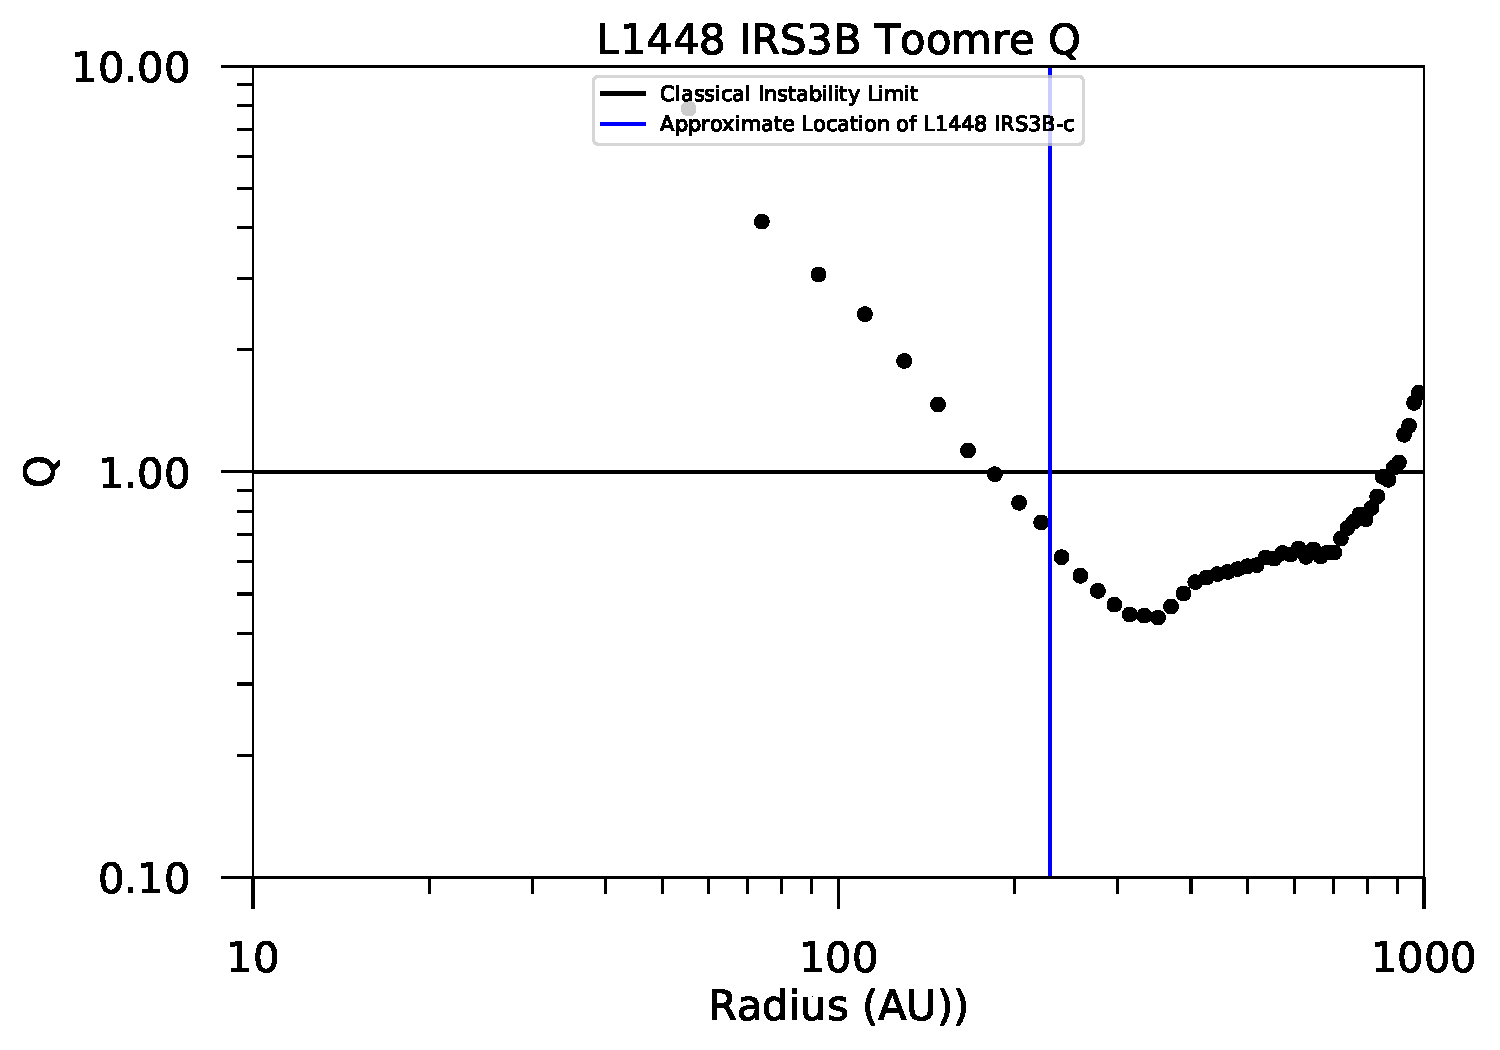
\includegraphics[width=0.48\textwidth]{img/L1448N-toomre-Q-linear-xsec-c17o_cont.pdf}
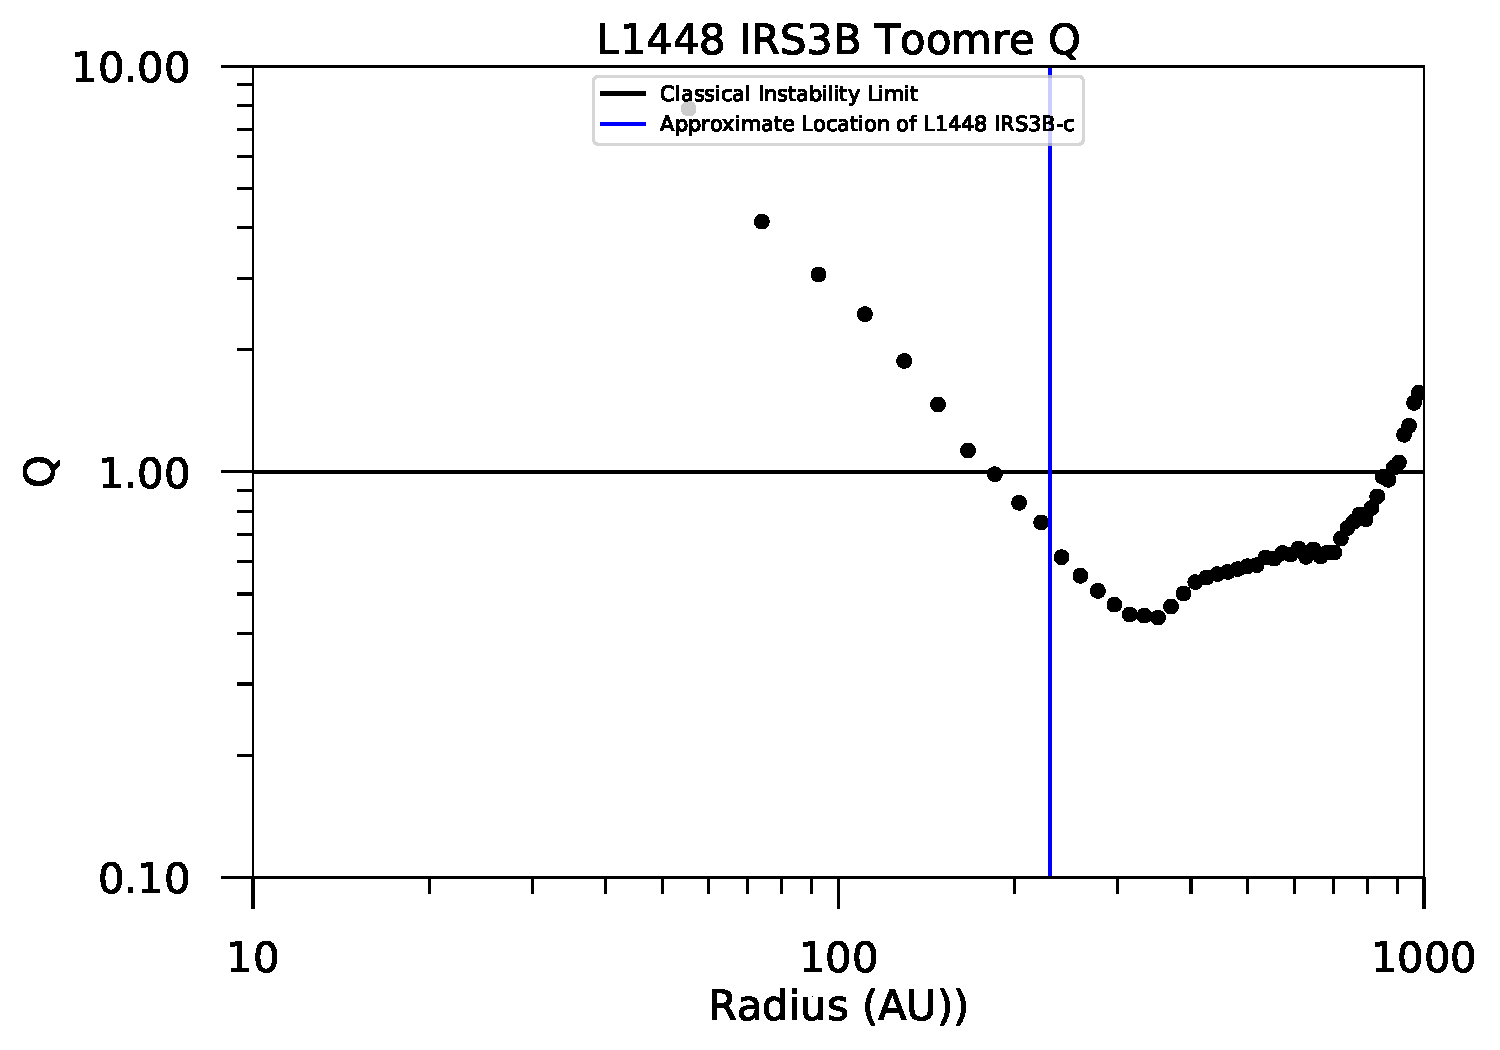
\includegraphics[width=0.48\textwidth]{img/L1448N-toomre-Q-linear-xsec-c17o_cont.pdf}
\end{center}   
\caption{Toomre Q parameter plotted as a function of deprojected radius for IRS3B. The horizontal line indicates a Toomre Q parameter of one, at which the disk would be gravitationally unstable. As indicated, the disk Toomre Q parameter drops below 1 at a radius of \ab120~AU. The vertical line corresponds to the deprojected radius of IRS3B-c. The observed spiral arms also become most prominent at R $>$100~AU, where Toomre~Q approaches 1.}\label{fig:irs3btoomreq}
\end{figure}

% figure 22
\begin{figure}[H]
\begin{center}
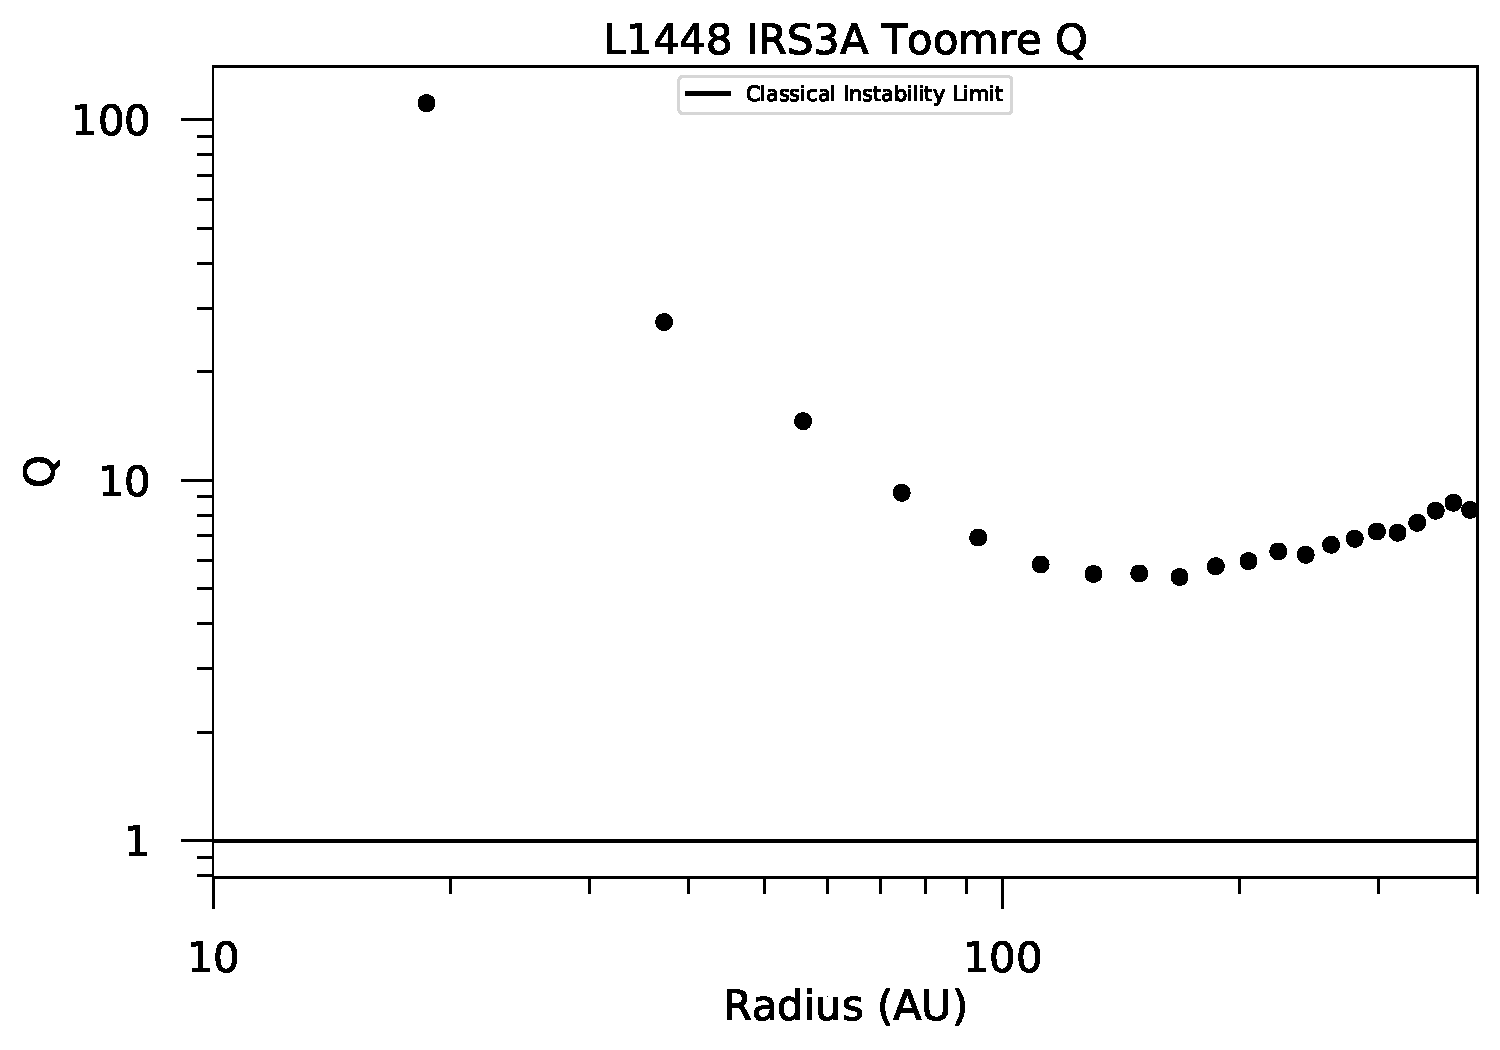
\includegraphics[width=0.48\textwidth]{img/L1448N-toomre-Q-linear-xsec-cont_robust-05_wide.pdf}
\end{center}   
\caption{Toomre Q parameter plotted as a function of deprojected radius for IRS3A. The horizontal line indicates a Toomre Q parameter of one, at which the disk would be gravitationally unstable. The circumstellar disk of IRS3A is much less massive than IRS3B, coupled with a \replaced{more massive central gravitational source}{protostar}, the disk is more stable against gravitational instabilities.}\label{fig:irs3atoomreq}
\end{figure}




% TODO: work on this
% IRS3B-ab outflow misalignment CO
% 28.5 - (90 - np.arccos(2.7871/17.0455) * 180. / np.pi)

\begin{figure}[H]
   \begin{center}
   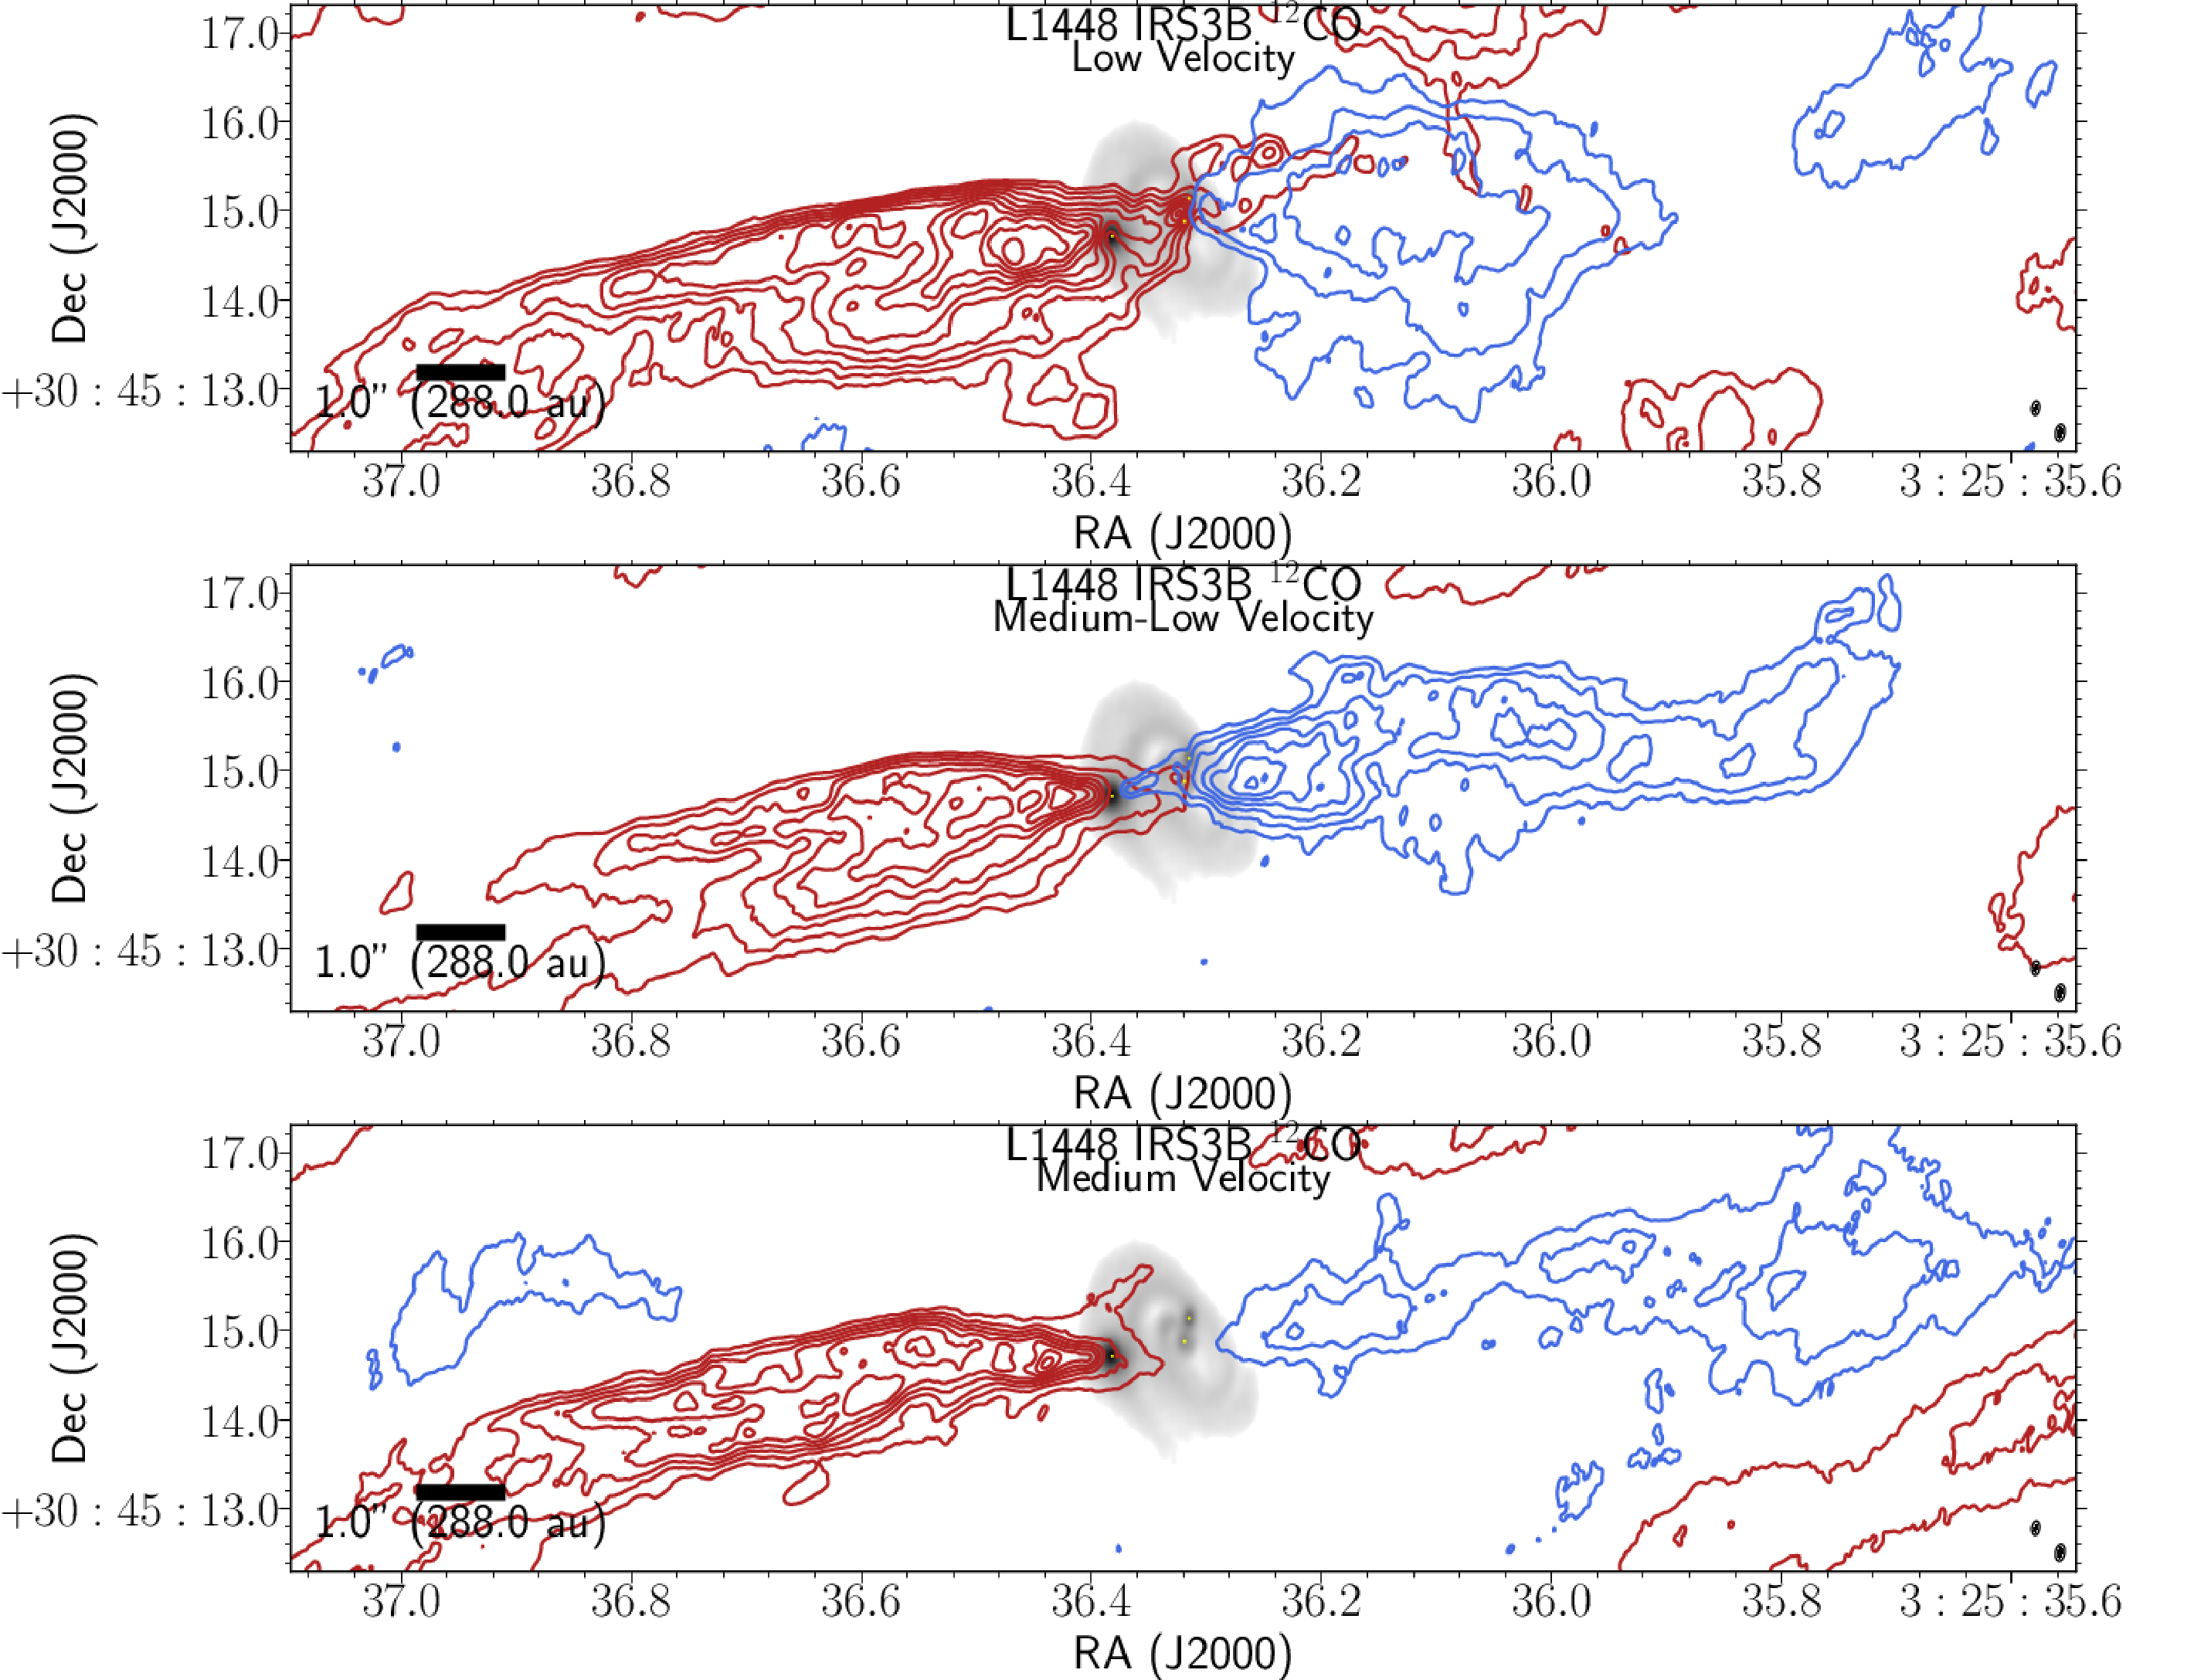
\includegraphics[width=\textwidth]{img/L1448IRS3B_12CO_image_binned_clean__binnedMoments_panel1.pdf}
   \caption{Moment 0 map (integrated intensity) of \co, overlaid on the continuum (grayscale) image from Figure~\ref{fig:contimage}, split up according to velocity ranges, providing exquisite detailing of the location and collimated of the IRS3B outflows. The central outflow from IRS3B extends 10\arcsec\space(2880~au)\added{, beyond the edge of the primary beam of ALMA at 879~micron,} from launch location on either side. The panels correspond to low, medium-low, and medium velocity ranges which are delineated as red(blue), respectively. \textbf{Low Velocity:} velocity ranges 5.5$\rightarrow$10.5~km~s$^{-1}$ (4$\rightarrow$-1~km~s$^{-1}$), contours start at 3(3)~$\sigma$ and iterate by 2(2)~$\sigma$ with the 1-$\sigma$~level starting at 0.1(0.1)~Jy~beam$^{-1}$ for the red(blue) channels respectively. \textbf{Medium-low Velocity:} velocity ranges 10.5$\rightarrow$15.5~km~s$^{-1}$ (-6$\rightarrow$-4~km~s$^{-1}$), contours start at 5(5)~$\sigma$ and iterate by 3(2)~$\sigma$ with the 1-$\sigma$~level starting at 0.04(0.004)~Jy~beam$^{-1}$ for the red(blue) channels respectively. \textbf{Medium Velocity:} velocity ranges 15.5$\rightarrow$20.5~km~s$^{-1}$ (-11$\rightarrow$-6~km~s$^{-1}$), contours start at 10(10)~$\sigma$ and iterate by 4(4)~$\sigma$ with the 1-$\sigma$~level starting at 0.02(0.02)~Jy~beam$^{-1}$ for the red(blue) channels respectively. The \co\space synthesized beam (\cobeam) is the bottom-right most overlay on each of the panels and the continuum synthesized beam (\contbeam) is offset diagonally.}\label{fig:comomentmap}
\end{center}
\end{figure}
\begin{figure}[H]
   \begin{center}
   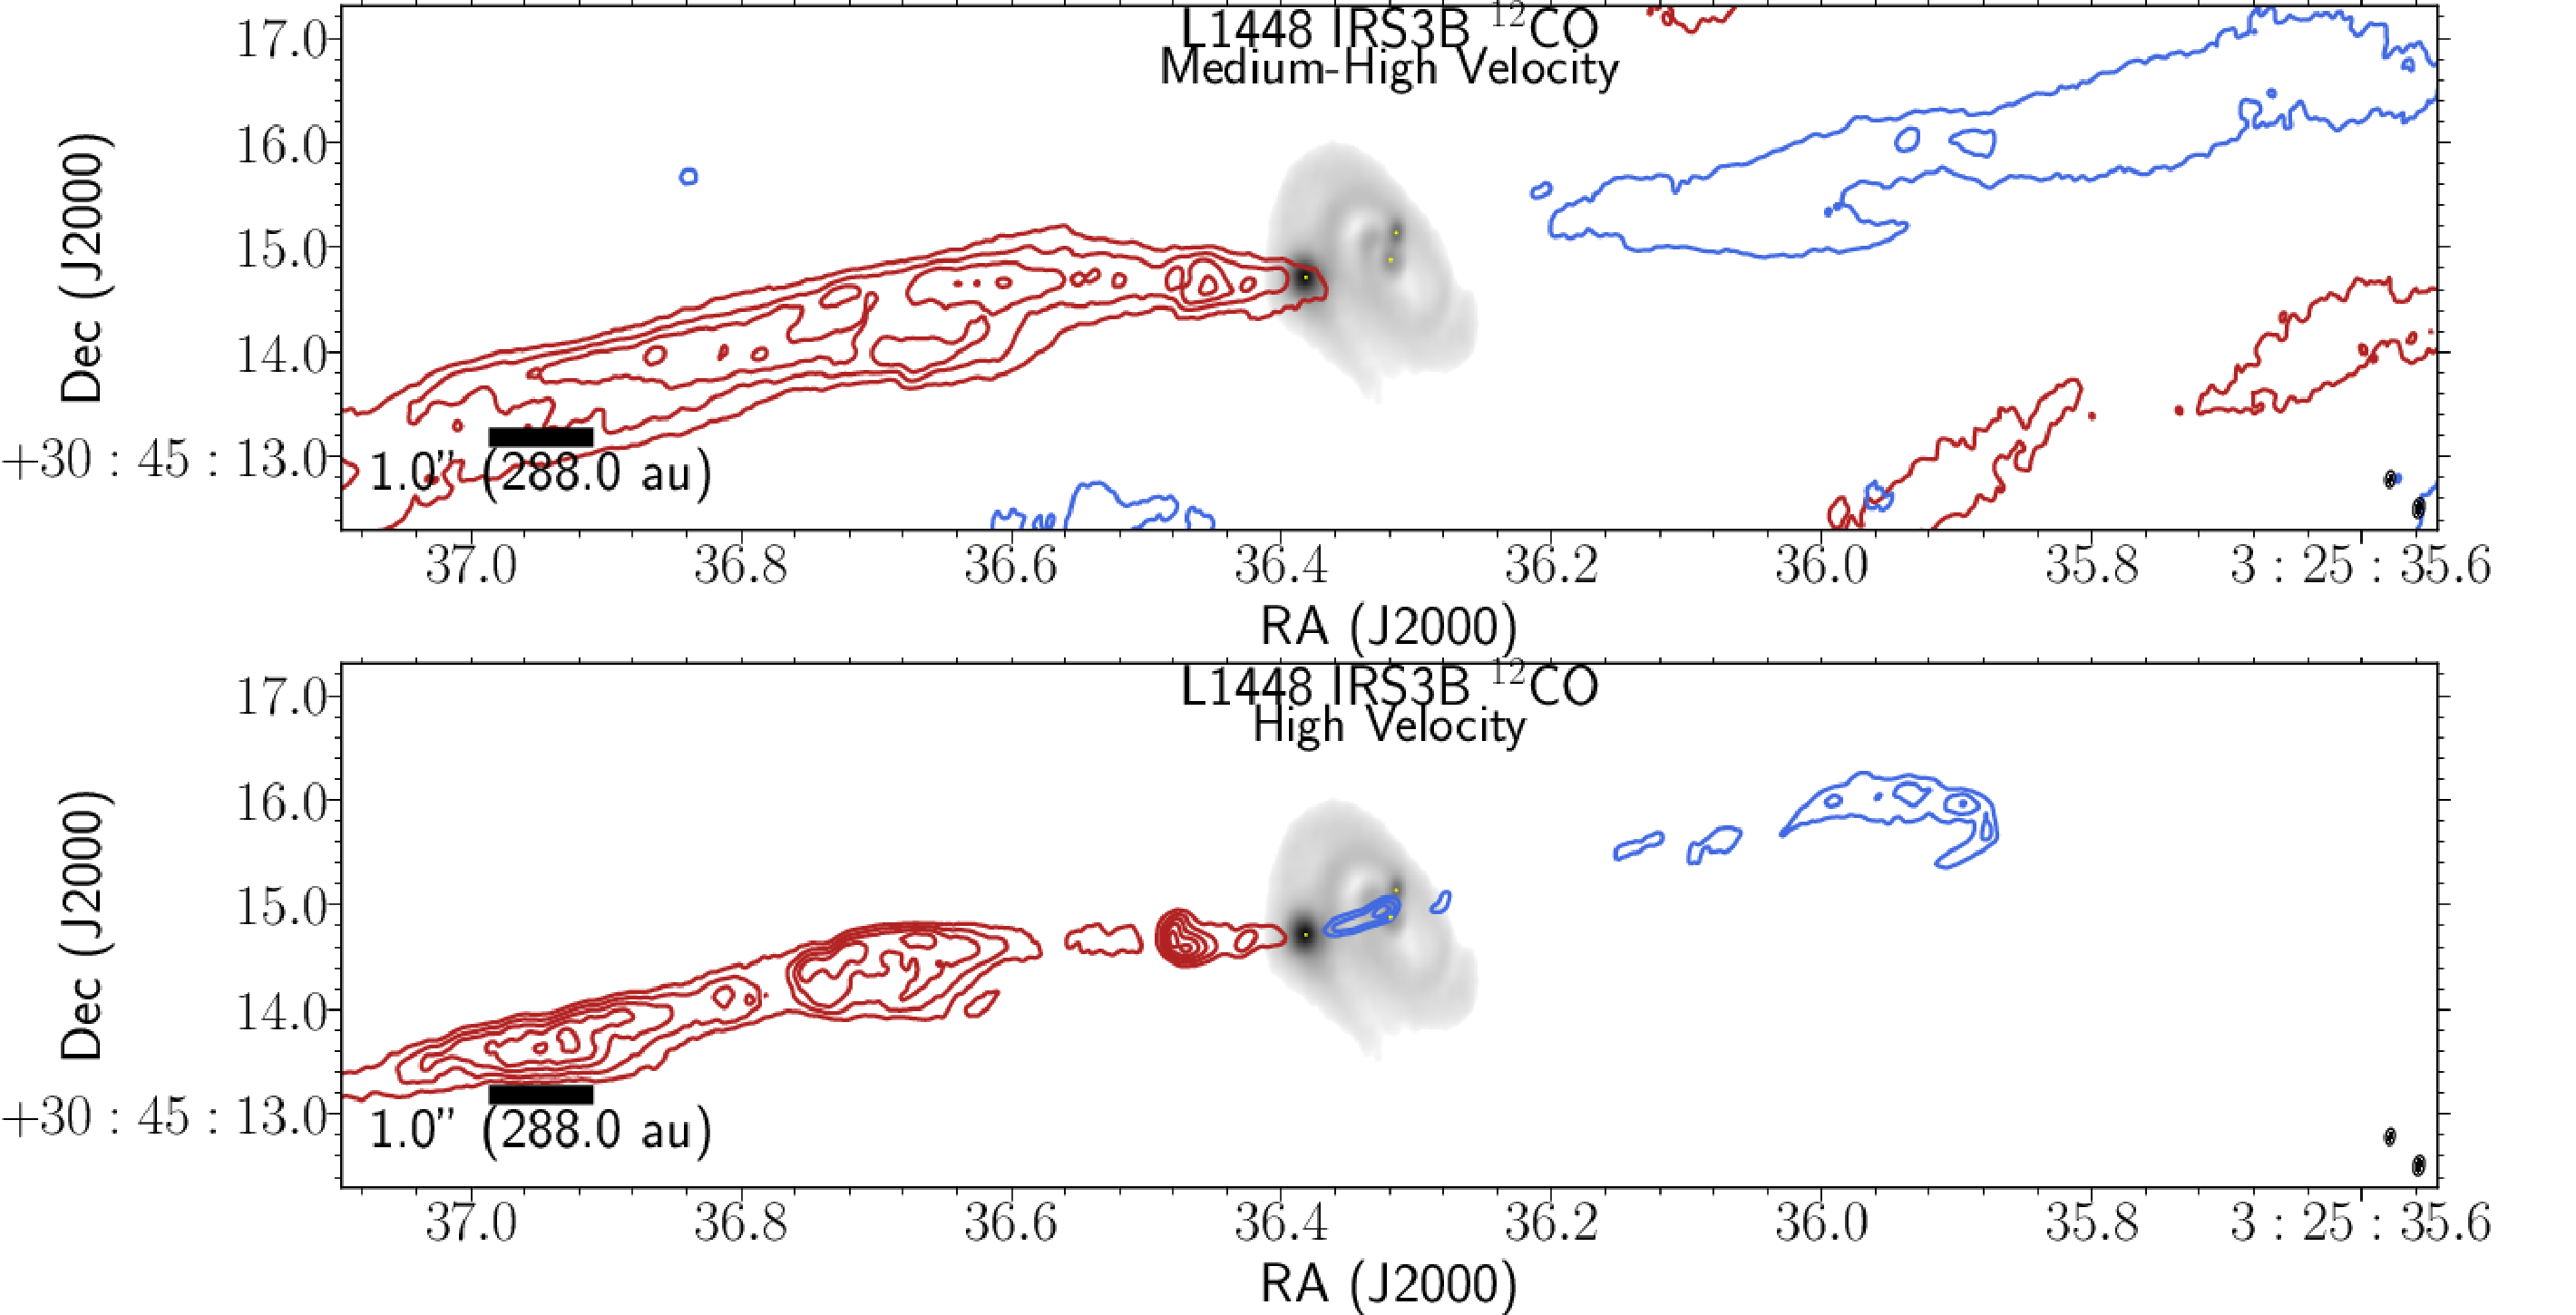
\includegraphics[width=\textwidth]{img/L1448IRS3B_12CO_image_binned_clean__binnedMoments_panel2.pdf}
   \caption{Same as Figure~\ref{fig:comomentmap} but for the \textbf{Medium-high Velocity:} velocity ranges 20.5$\rightarrow$25.5~km~s$^{-1}$ (-16$\rightarrow$-11~km~s$^{-1}$), contours start at 3(3)~$\sigma$ and iterate by 4(4)~$\sigma$ with the 1-$\sigma$~level starting at 0.04(0.04)~Jy~beam$^{-1}$ for the red(blue) channels respectively. \textbf{High Velocity:} velocity ranges 25.5$\rightarrow$30.5~km~s$^{-1}$ (-21$\rightarrow$-16~km~s$^{-1}$), contours start at 5(5)~$\sigma$ and iterate by 2(2)~$\sigma$ with the 1-$\sigma$~level starting at 0.04(0.04)~Jy~beam$^{-1}$ for the red(blue) channels respectively. The \co\space synthesized beam (\cobeam) is the bottom-right most overlay on each of the panels and the continuum synthesized beam (\contbeam) is offset diagonally.}\label{fig:comomentmap2}
\end{center}
\end{figure}

\begin{figure}[H]
   \begin{center}
   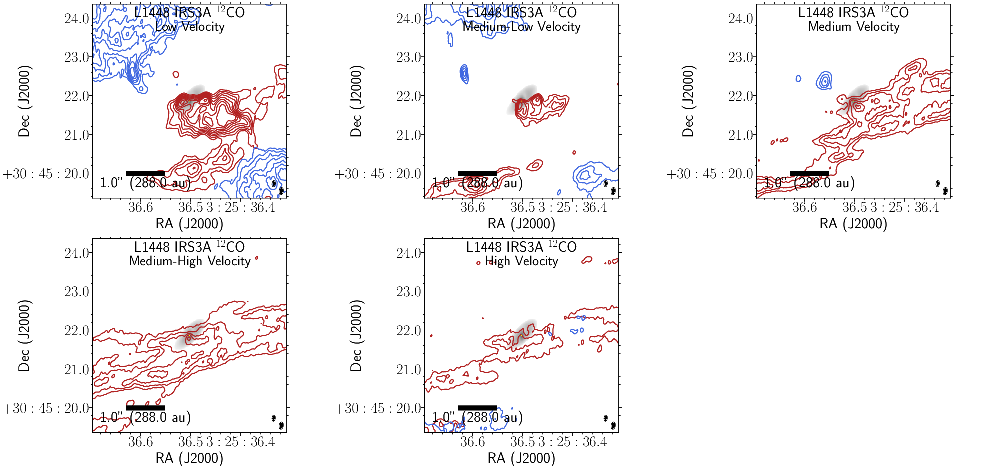
\includegraphics[width=\textwidth]{img/L1448IRS3B_12CO_image_binned_clean-montage-irs3a.pdf}
   \caption{Similar to Figures~\ref{fig:comomentmap}~and~\ref{fig:comomentmap2} towards the IRS3A source with the same velocity ranges. \textbf{Low Velocity:} velocity ranges 5.5$\rightarrow$10.5~km~s$^{-1}$ (4$\rightarrow$-1~km~s$^{-1}$), contours start at 5(5)~$\sigma$ and iterate by 4(2)~$\sigma$ with the 1-$\sigma$~level starting at 0.1(0.1)~Jy~beam$^{-1}$ for the red(blue) channels respectively. \textbf{Medium-low Velocity:} velocity ranges 10.5$\rightarrow$15.5~km~s$^{-1}$ (-6$\rightarrow$-4~km~s$^{-1}$), contours start at 5(5)~$\sigma$ and iterate by 2(2)~$\sigma$ with the 1-$\sigma$~level starting at 0.04(0.004)~Jy~beam$^{-1}$ for the red(blue) channels respectively. \textbf{Medium Velocity:} velocity ranges 15.5$\rightarrow$20.5~km~s$^{-1}$ (-11$\rightarrow$-6~km~s$^{-1}$), contours start at 5(5)~$\sigma$ and iterate by 2(2)~$\sigma$ with the 1-$\sigma$~level starting at 0.02(0.02)~Jy~beam$^{-1}$ for the red(blue) channels respectively. \textbf{Medium-high Velocity:} velocity ranges 20.5$\rightarrow$25.5~km~s$^{-1}$ (-16$\rightarrow$-11~km~s$^{-1}$), contours start at 3(3)~$\sigma$ and iterate by 2(2)~$\sigma$ with the 1-$\sigma$~level starting at 0.04(0.04)~Jy~beam$^{-1}$ for the red(blue) channels respectively. \textbf{High Velocity:} velocity ranges 25.5$\rightarrow$30.5~km~s$^{-1}$ (-21$\rightarrow$-16~km~s$^{-1}$), contours start at 3(3)~$\sigma$ and iterate by 2(2)~$\sigma$ with the 1-$\sigma$~level starting at 0.04(0.04)~Jy~beam$^{-1}$ for the red(blue) channels respectively. The \co\space synthesized beam (\cobeam) is the bottom-right most overlay on each of the panels and the continuum synthesized beam (\contbeam) is offset diagonally.}\label{fig:comomentmapirs3a}
\end{center}
\end{figure}

\begin{figure}[H]
   \begin{center}
   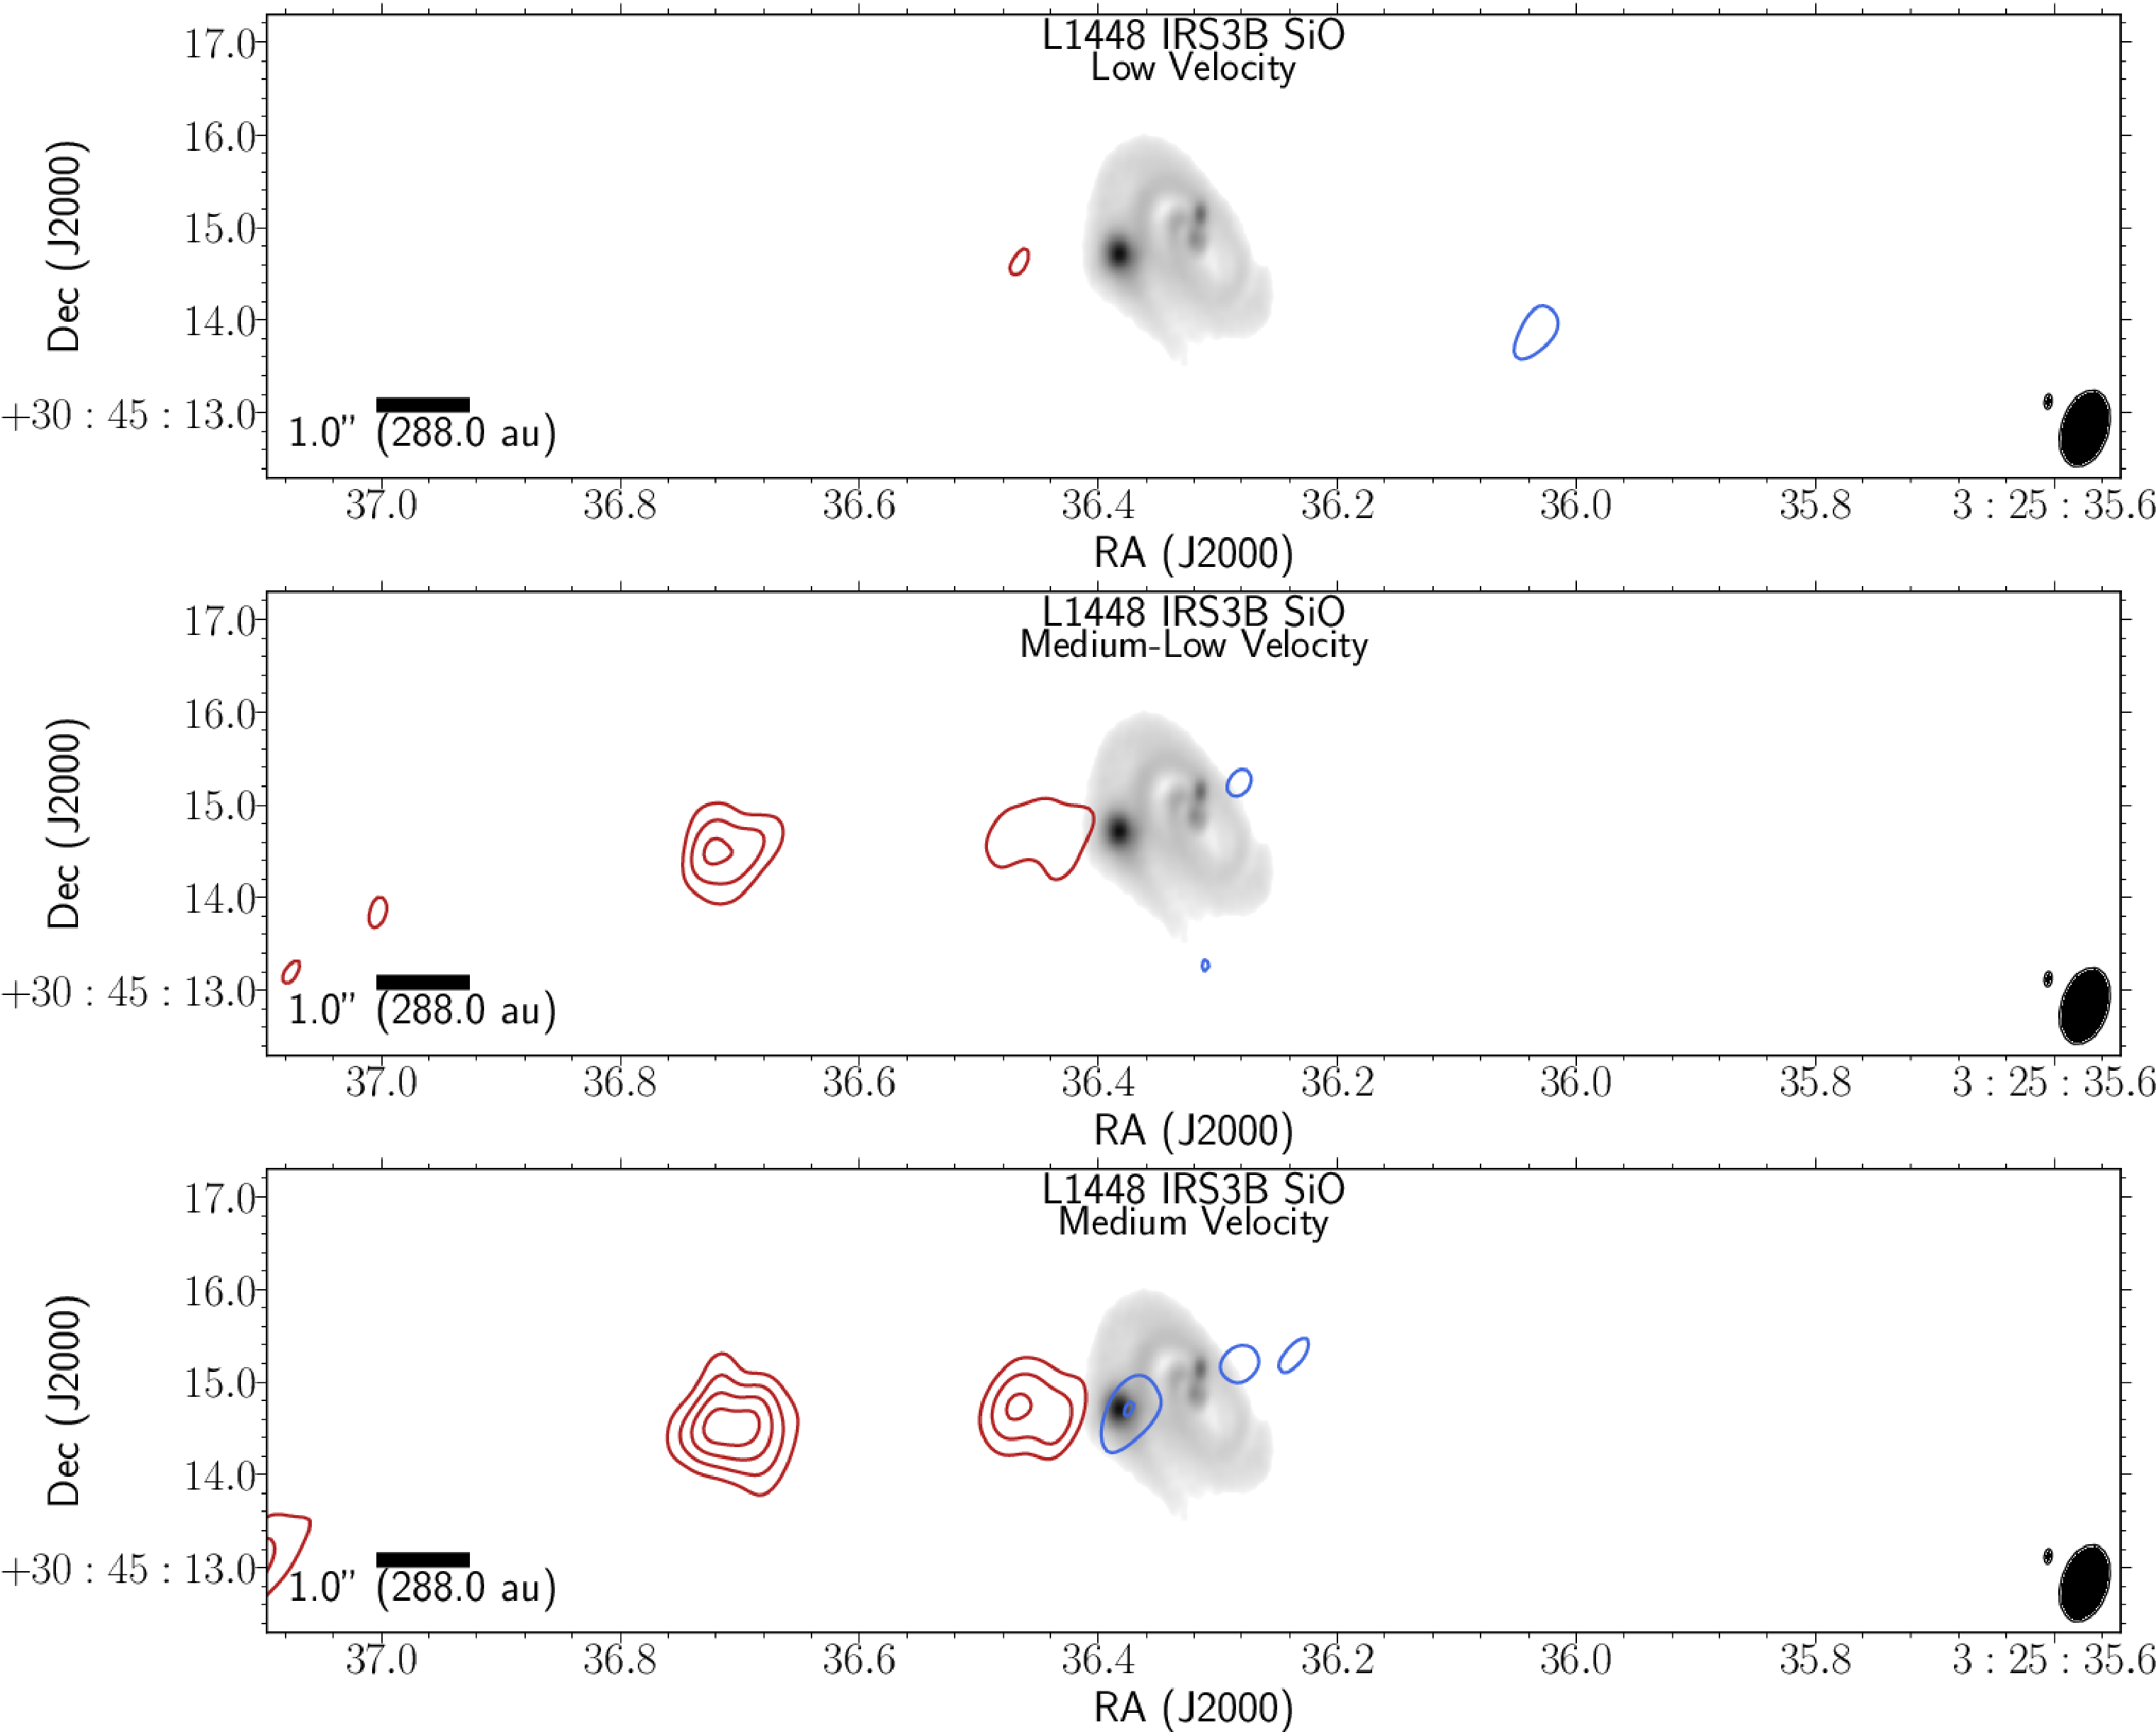
\includegraphics[width=\textwidth]{img/L1448IRS3B_SiO_image_taper1500k__panel1.pdf} % co
   \end{center}
   \caption{Moment 0 map (integrated intensity) of \sio, overlaid on the continuum (grayscale) image from Figure~\ref{fig:contimage}. \sio\space shows locations of shocked gas fronts. There is significant blue-shifted emission on the eastern side of the image, in the same location as the red-shifted outflow, which is coming from the L1448-C outflow, located \ab3\arcmin south of L1448 IRS3B. The panels correspond to low, medium-low, and medium velocity ranges which are delineated as red(blue), respectively. \textbf{Low Velocity:} velocity ranges 5.5$\rightarrow$10.5~km~s$^{-1}$ (4$\rightarrow$-1~km~s$^{-1}$), contours start at 5(5)~$\sigma$ and iterate by 3(3)~$\sigma$ with the 1-$\sigma$~level starting at 0.11(0.09)~Jy~beam$^{-1}$ for the red(blue) channels respectively. \textbf{Medium-low Velocity:} velocity ranges 10.5$\rightarrow$15.5~km~s$^{-1}$ (-6$\rightarrow$-4~km~s$^{-1}$), contours start at 5(5)~$\sigma$ and iterate by 3(3)~$\sigma$ with the 1-$\sigma$~level starting at 0.01(0.01)~Jy~beam$^{-1}$ for the red(blue) channels respectively. \textbf{Medium Velocity:} velocity ranges 15.5$\rightarrow$20.5~km~s$^{-1}$ (-11$\rightarrow$-6~km~s$^{-1}$), contours start at 5(5)~$\sigma$ and iterate by 3(3)~$\sigma$ with the 1-$\sigma$~level starting at 0.009(0.012)~Jy~beam$^{-1}$ for the red(blue) channels respectively. The \sio\space synthesized beam (\siobeam) is the bottom-right most overlay on each of the panels and the continuum synthesized beam (\contbeam) is offset diagonally.}\label{fig:siomomentmap}
\end{figure}

\begin{figure}[H]
   \begin{center}
   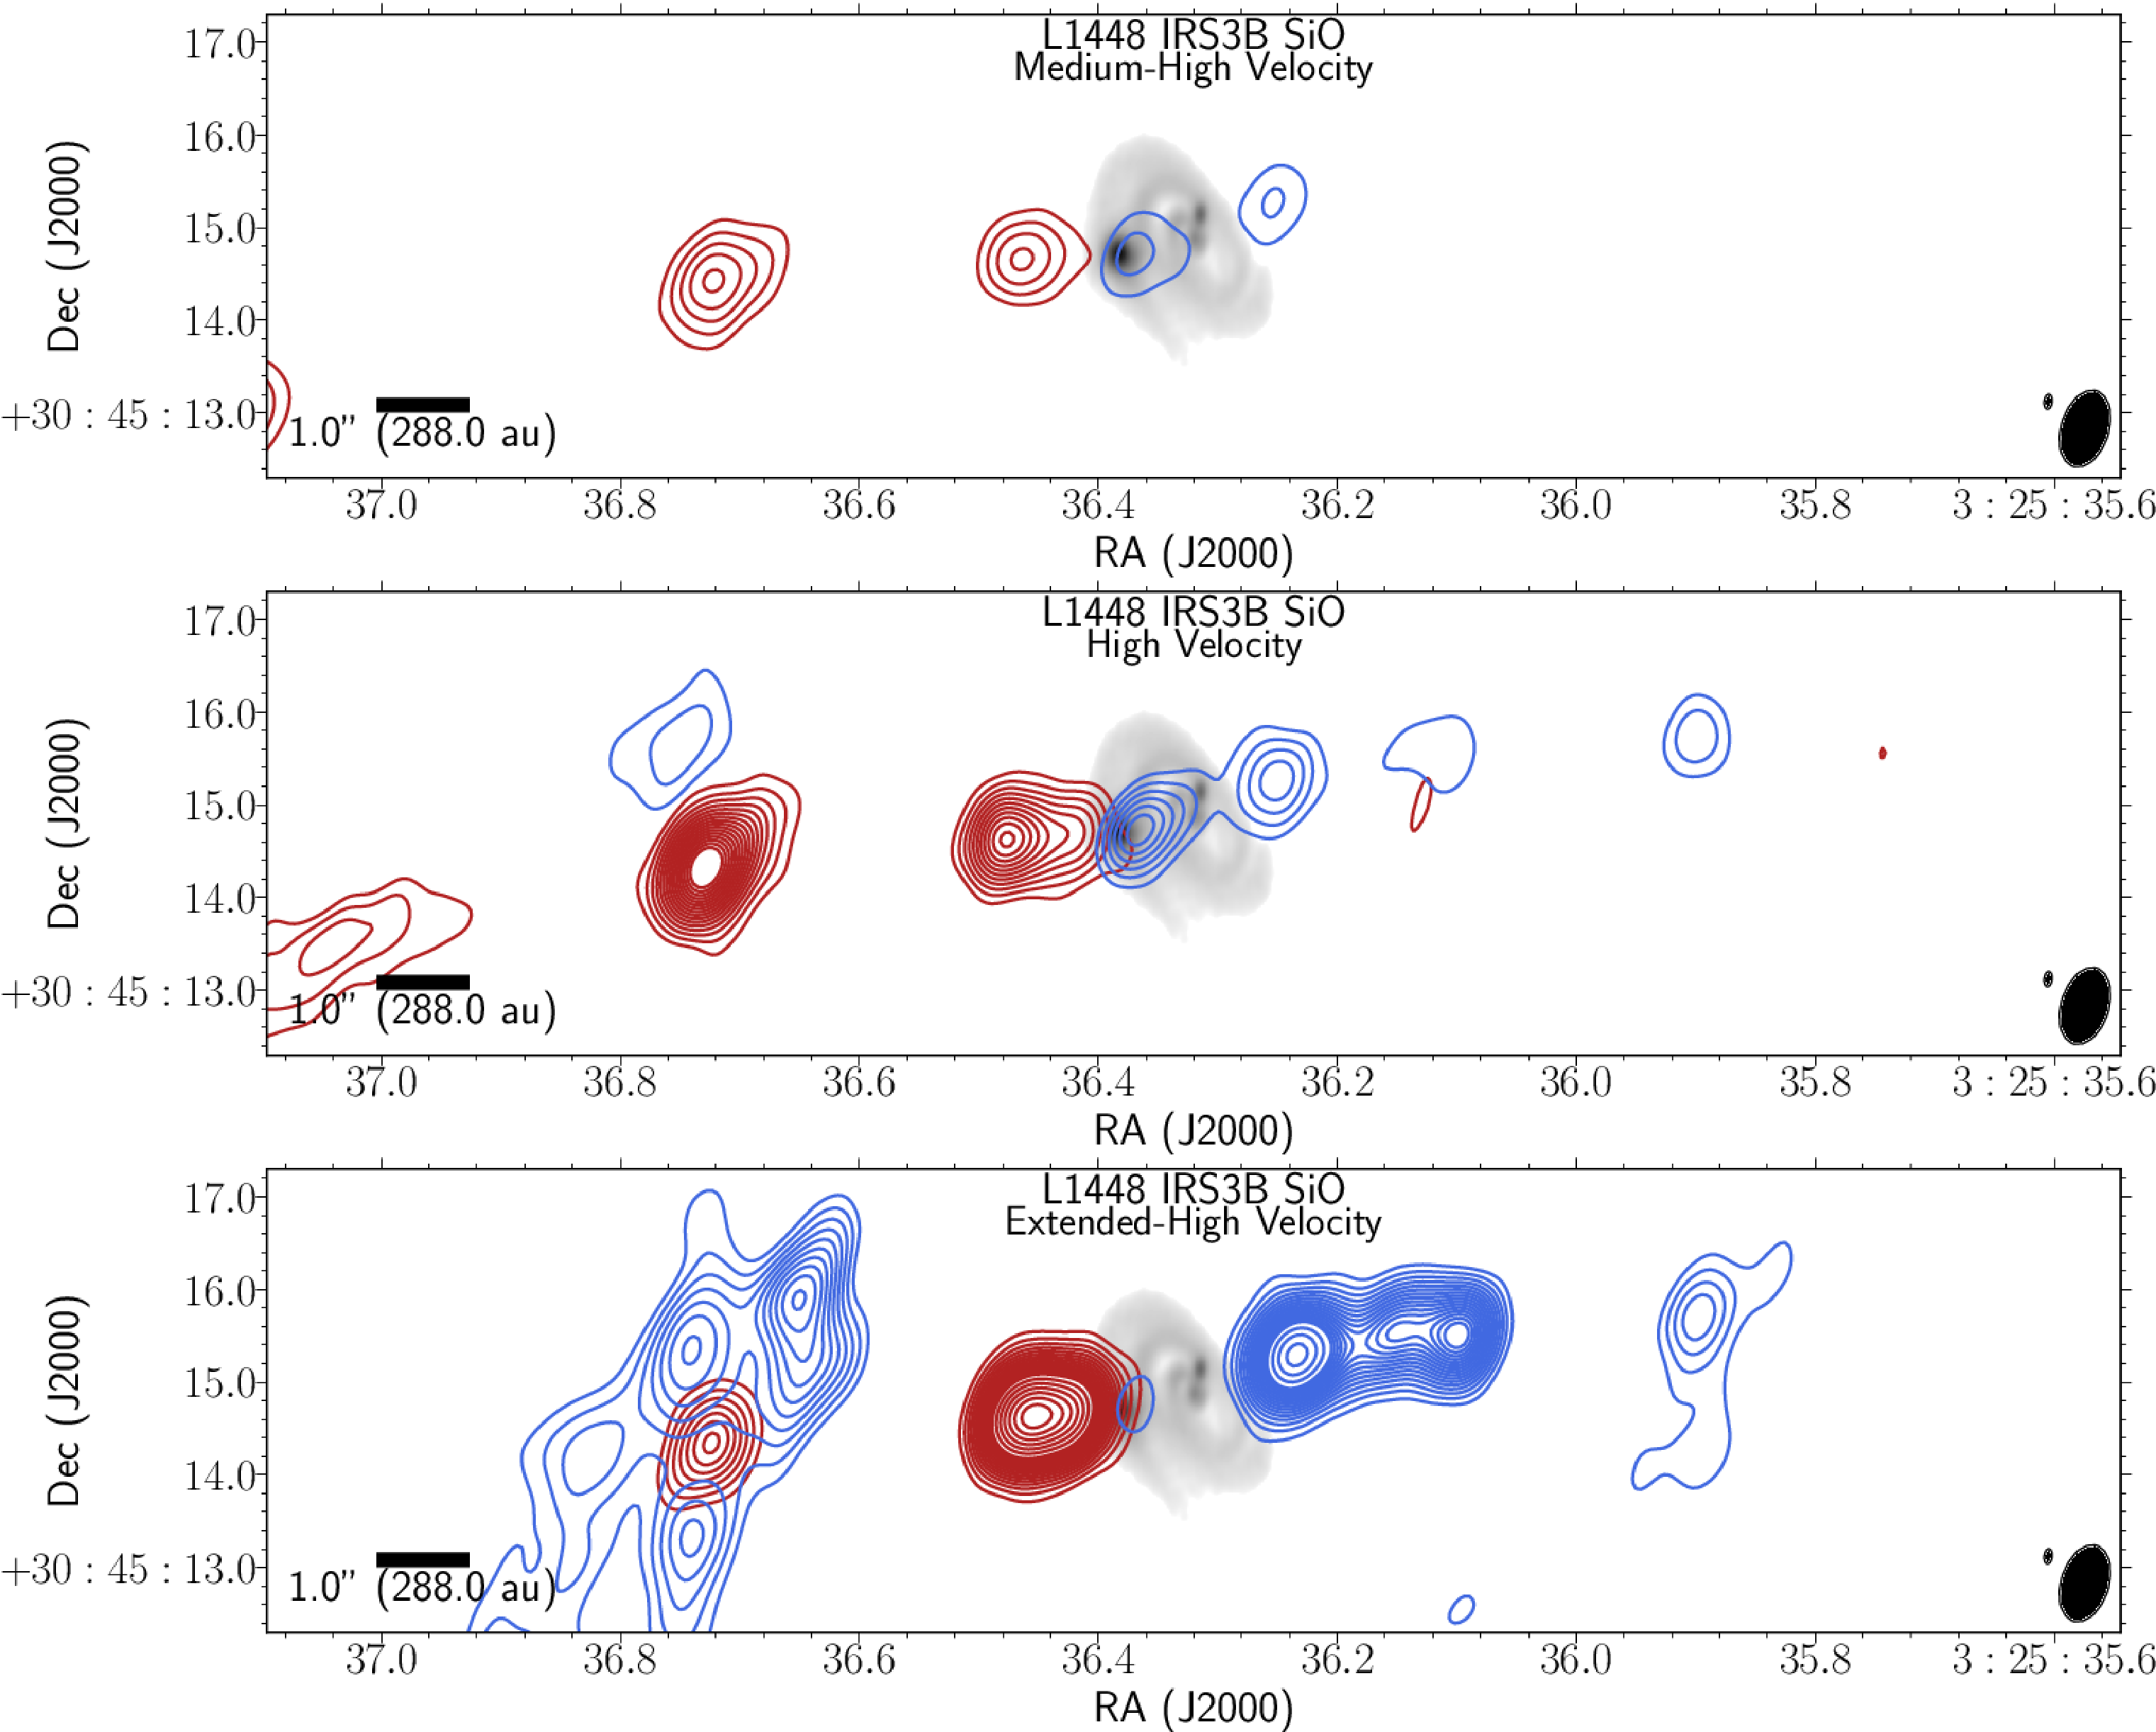
\includegraphics[width=\textwidth]{img/L1448IRS3B_SiO_image_taper1500k__panel2.pdf} % co
   \end{center} 
   \caption{Similar to Figure~\ref{fig:siomomentmap} but for the \textbf{Medium-high Velocity:} velocity ranges 20.5$\rightarrow$25.5~km~s$^{-1}$ (-16$\rightarrow$-11~km~s$^{-1}$), contours start at 5(5)~$\sigma$ and iterate by 3(3)~$\sigma$ with the 1-$\sigma$~level starting at 0.012(0.015)~Jy~beam$^{-1}$ for the red(blue) channels respectively. \textbf{High Velocity:} velocity ranges 25.5$\rightarrow$30.5~km~s$^{-1}$ (-21$\rightarrow$-16~km~s$^{-1}$), contours start at 5(5)~$\sigma$ and iterate by 3(3)~$\sigma$ with the 1-$\sigma$~level starting at 0.008(0.015)~Jy~beam$^{-1}$ for the red(blue) channels respectively. \textbf{Extended-High Velocity:} velocity ranges 30.5$\rightarrow$50~km~s$^{-1}$ (-40$\rightarrow$-21~km~s$^{-1}$), contours start at 5(5)~$\sigma$ and iterate by 3(3)~$\sigma$ with the 1-$\sigma$~level starting at 0.025(0.025)~Jy~beam$^{-1}$ for the red(blue) channels respectively. The \sio\space has additional emission well beyond the velocity range of the emission in \co\space and is presented as an additional panel (``extended-high velocity'') which only features the red-shifted emission. The \sio\space synthesized beam (\siobeam) is the bottom-right most overlay on each of the panels and the continuum synthesized beam (\contbeam) is offset diagonally. }\label{fig:siomomentmap2}
\end{figure}
